\documentclass[default,iicol]{sn-jnl}

\usepackage{epsfig} %% for loading postscript figures
\usepackage{array}
\usepackage{amsmath}
\usepackage{xcolor}
\usepackage{subfig}
\usepackage{float}
%\usepackage{caption}
\usepackage{titlesec}
\usepackage{stfloats}

\setcounter{secnumdepth}{4}

\titleformat{\paragraph}
{\normalfont\normalsize\bfseries}{\theparagraph}{1em}{}
\titlespacing*{\paragraph}
{0pt}{3.25ex plus 1ex minus .2ex}{1.5ex plus .2ex}

%\def\url#1{\expandafter\string\csname #1\endcsname}
\usepackage{url}
\newcounter{exno}
\newenvironment{examples}
{
\begin{flushleft}
\begin{tabular}{>{(\refstepcounter{exno}\theexno\label{row:\theexno}) }rl}
}
{
\end{tabular}
\end{flushleft}
}
%\newcommand*{\@rowstyle}{}
\newcommand*{\rowstyle}[1]{% sets the style of the next row
  \gdef\@rowstyle{#1}%
  \@rowstyle\ignorespaces%
}
\newcolumntype{=}{% resets the row style
  >{\gdef\@rowstyle{}}%
}
\newcolumntype{+}{% adds the current row style to the next column
  >{\@rowstyle}%
}
\definecolor{ao}{rgb}{0.0, 0.5, 0.0}
\definecolor{coolblack}{rgb}{0.0, 0.18, 0.39}

% \usepackage{fancyhdr}% http://ctan.org/pkg/fancyhdr

% % \fancyhf{}% Clear header/footer
% % \fancyhead[R]{\sectionmark}
% % \fancyfoot[C]{\thepage}% \fancyfoot[R]{\thepage}
% % \renewcommand{\headrulewidth}{0.4pt}% Default \headrulewidth is 0.4pt

% % \renewcommand{\sectionmark}[1]{\markright{\thesection~- ~#1}}
% % \renewcommand{\chaptermark}[1]{\markboth{\chaptername~\thechapter~-~ #1}{}}
% \renewcommand{\subsectionmark}[1]{\markright{#1}}

% %\usepackage[T1]{fontenc}
% \usepackage{bold-extra}


% % % Fancyhdr setup
% % \pagestyle{fancy}% Change page style to fancy
% % \fancyhf{} % clear all header fields
% % \fancyhead[L]{\footnotesize\scshape\leftmark}
% % \fancyhead[R]{\footnotesize\scshape\rightmark}
% % \fancyfoot[C]{\thepage}
% % \renewcommand{\headrulewidth}{0.4 pt}
% % \renewcommand{\footrulewidth}{0 pt}

\newcounter{magicrownumbers}
\newcommand\rownumber{\stepcounter{magicrownumbers}\arabic{magicrownumbers}}

\jyear{2021}%

%% as per the requirement new theorem styles can be included as shown below
\theoremstyle{thmstyleone}%
\newtheorem{theorem}{Theorem}%  meant for continuous numbers
%%\newtheorem{theorem}{Theorem}[section]% meant for sectionwise numbers
%% optional argument [theorem] produces theorem numbering sequence instead of independent numbers for Proposition
\newtheorem{proposition}[theorem]{Proposition}% 
%%\newtheorem{proposition}{Proposition}% to get separate numbers for theorem and proposition etc.

\theoremstyle{thmstyletwo}%
\newtheorem{example}{Example}%
\newtheorem{remark}{Remark}%

\theoremstyle{thmstylethree}%
\newtheorem{definition}{Definition}%

\raggedbottom
%%\unnumbered% uncomment this for unnumbered level heads

\begin{document}

\title[]{\vspace{-3cm}Optimal Skateboard Geometry for Maximizing Ollie Height}

%%=============================================================%%
%% Prefix	-> \pfx{Dr}
%% GivenName	-> \fnm{Joergen W.}
%% Particle	-> \spfx{van der} -> surname prefix
%% FamilyName	-> \sur{Ploeg}
%% Suffix	-> \sfx{IV}
%% NatureName	-> \tanm{Poet Laureate} -> Title after name
%% Degrees	-> \dgr{MSc, PhD}
%% \author*[1,2]{\pfx{Dr} \fnm{Joergen W.} \spfx{van der} \sur{Ploeg} \sfx{IV} \tanm{Poet Laureate} 
%%                 \dgr{MSc, PhD}}\email{iauthor@gmail.com}
%%=============================================================%%

\author*[1,2]{\fnm{Jan T.} \sur{Heinen}}\email{janheinen97@gmail.com}

\author[2,3]{\fnm{Jason K.} \sur{Moore}}\email{j.k.moore@tudelft.com}
\equalcont{These authors contributed equally to this work.}

\author[1,2]{\fnm{Eline} \sur{van der Kruk}}\email{e.vanderkruk@tudelft.com}
\equalcont{These authors contributed equally to this work.}

\affil*[1]{\orgdiv{Department of Biomechanical Engineering}, \orgname{TU Delft}, \orgaddress{\street{Street}, \city{City}, \postcode{100190}, \state{State}, \country{Country}}}

\affil[2]{\orgdiv{Department}, \orgname{Organization}, \orgaddress{\street{Street}, \city{City}, \postcode{10587}, \state{State}, \country{Country}}}

%\abstract{Skateboarding involves a human controlling a four wheeled vehicle that is steered by tilting the standing surface. The riding mechanics of skateboarding have been well reported \cite{hubbard_clearing_1985,varszegi_stabilizing_2016}. The sport also includes aerial maneuvers such as jumping of stairs, flying off ramps and flipping and rotating the skateboard. The most basic aerial trick is called the ollie. The athlete jumps up while pushing down on the back end of the skateboard’s tail, causing a rotation about the back axle. The upward acceleration due to the rotation together with the tail-ground impact cause the skateboard to go airborne. Midair the athlete drags the skateboard up through frictional contact and levels it out to land the trick. The most concrete performance measure of the ollie is height according to the Olympic judging criteria\cite{world_skate_skateboarding_2021}. To reach maximum height the dynamics such as impact, dynamic response, and torque production are dependent on shape, inertia and mass, which gives reason to assume an optimal shape exists. This leads to the research question: What are the optimal geometric and inertial parameters of a skateboard for an Olympic athlete to reach maximal ollie height. The skateboard geometry is optimized through multiphase direct collocation with the objective of maximal ollie height. A parameterized model is created with scaling mass and inertia properties such that the geometry of the skateboard. Modelling the dynamics of the ollie including impact and friction are done with a point mass human controller that is kineticly and kinematicly mapped to a counter movement jump. A simplistic contact implicit impact scheme is made for a higher order optimization. The ollie height is improved by changing the mass and inertia properties of the skateboard. Multiple optimal board shapes are generated for example a skateboard with a smaller wheelbase can reach higher ollie height compared to an industry standard skateboard.}

\keywords{Skateboarding, Optimal Control, Parameter Optimization, Direct Collocation}
\maketitle

\section{Introduction}\label{s_intro}

In 1978 Alan `Ollie' Gelfand invented the `no-hand aerial', by riding of an
inclined surface and jumping in the air with a skateboard. Later Rodney Mullen
was known for inventing the ollie from flat ground. The ollie, is a skateboard
trick that intends to bring the skater with skateboard up. Because the
skateboard is not tethered to the skater in any way, a precise sequence of
movements is needed to keep the skater and skateboard together
\cite{frederick_biomechanics_2006}. The maneuver can be described in six
distinct phases which are shown in figure \ref{fig:ollie_steps}.

The ollie phases are (A)`Preparation': athlete lowers their centre of mass(COM)
prepares muscles for upward acceleration. (B) `Pre-pop': skateboard rotates
about it's wheels due to force of back foot. (C) `Pop': tail of the skateboard
hits the ground. Skater takes advantage of the collision between the skateboard
and ground to bring the skateboard up. (D) `Upward motion': the skater and
skateboard are both airborne. (E) `Downward motion': the legs are extended to
ensure a firm landing. (F) `Landing': the skater absorbs the impact.

\begin{figure*}[t]
\captionsetup[subfigure]{labelformat=empty}
  \subfloat[$t_1$=0.013]{{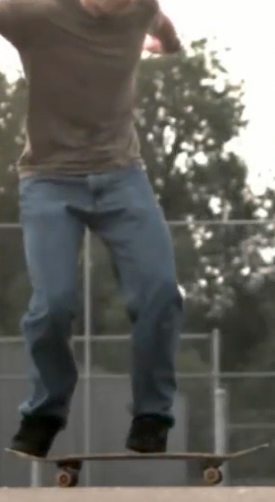
\includegraphics[width=0.13\textwidth]{figure/1.png} }}%
  \subfloat[$t_2$=0.129]{{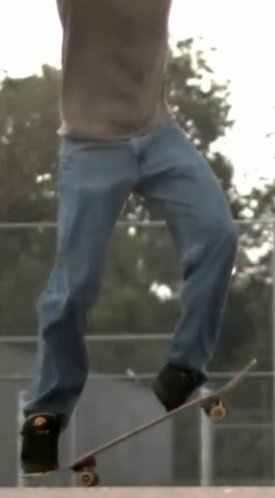
\includegraphics[width=0.13\textwidth]{figure/2.png} }}%
  \subfloat[$t_3$=0.181]{{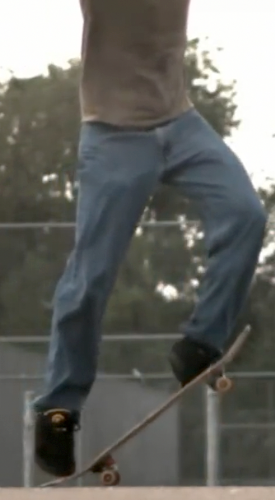
\includegraphics[width=0.13\textwidth]{figure/3.png} }}%
  \subfloat[$t_4$=0.187]{{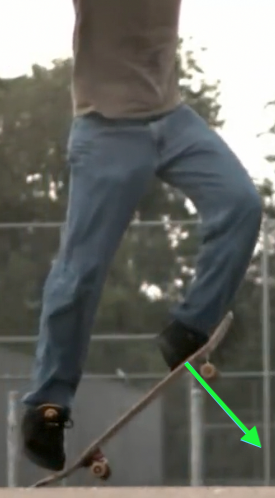
\includegraphics[width=0.13\textwidth]{figure/4.png} }}%
  \subfloat[$t_5$=0.303]{{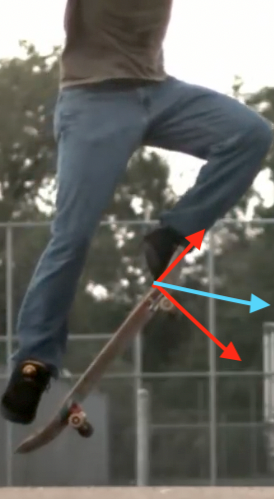
\includegraphics[width=0.13\textwidth]{figure/5.png} }}%
  \subfloat[$t_6$=0.431]{{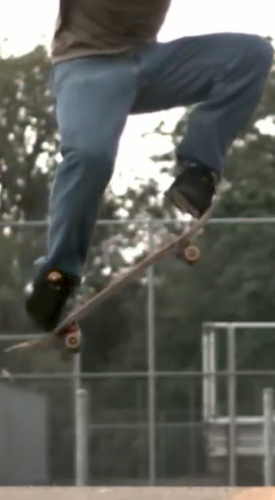
\includegraphics[width=0.13\textwidth]{figure/6.png} }}%
  \subfloat[$t_7$=0.543]{{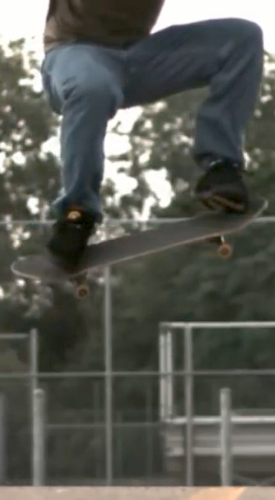
\includegraphics[width=0.13\textwidth]{figure/7.png} }}%
  \protect\newline
  \centering
  \subfloat[$t_8$=0.676$^1$]{{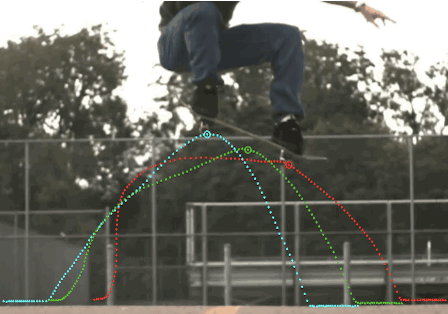
\includegraphics[width=0.336\textwidth]{figure/ollie_tracking_mid.png} }}
  \subfloat[$t_9$=0.722]{{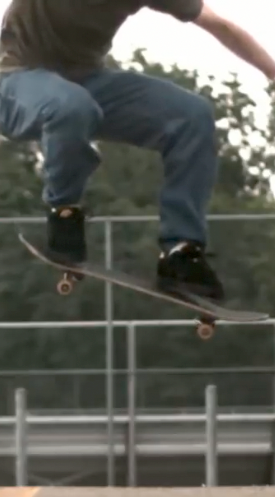
\includegraphics[width=0.13\textwidth]{figure/9.png} }}%
  \subfloat[$t_{10}$=0.904]{{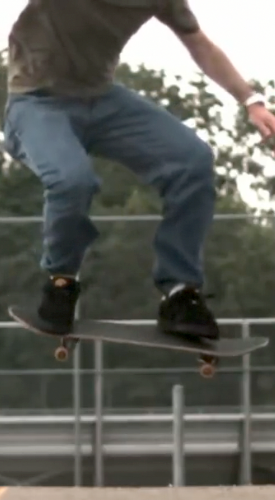
\includegraphics[width=0.13\textwidth]{figure/10.png} }}%
  \subfloat[$t_{11}$=1.097]{{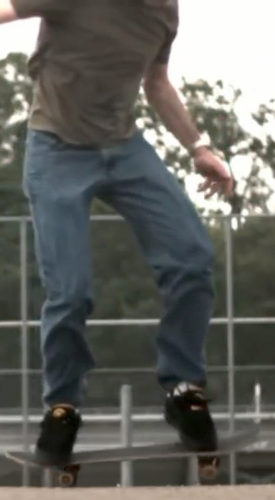
\includegraphics[width=0.13\textwidth]{figure/11.png} }}%
  \captionsetup{singlelinecheck=off}
  \vspace{-0.2cm}\caption[Ollie motion cues]{Green arrow: resultant force
    without friction, red arrows: force components with friction, blue arrow:
    resultant force with friction. Blue-, green- and red line are trajectory of
    back wheel, middle and front wheel respectively
    \footnotesize
    \begin{itemize}
      \item[$t_1$] The skater is pushing firmly from his back leg and is starting
        to have less force on the front foot which results in the wheel just
        leaving the ground.
      \item[$t_2$] The front foot starts sliding relative to the board for the
        first time.
      \item[$t_3$] Tail collides with the ground, the front foot is still sliding
        and the back foot is barely in contact with the skateboard.
      \item[$t_4$] Back foot is no longer in contact with the skateboard, the
        back wheels are not in contact with the ground anymore.
      \item[$t_5$] The front foot reached the nose of the skateboard.
      \item[$t_6$] Back foot contacts the board again.
      \item[$t_7$] Board is leveled out by the front foot.
      \item[$t_8$] Highest point is reached. Knees are fully tucked in. Feet are
        firmly placed on the deck.
      \item[$t_9$] Front foot loses contact.
      \item[$t_{10}$] Board is horizontal, both feet are in contact.
      \item[$t_{11}$] The back wheels touch the ground and legs are almost fully streched out.
      \item[$^1$] \url{https://www.wired.com/2014/10/skateboard-physics-empzeal}
      \item[$^2$] \url{https://www.youtube.com/watch?v=339k4XEvbxY}
    \end{itemize}
  }
  \label{fig:olliesteps}
\end{figure*}

The skateboard evolved from the early 1960s with different motives. New pursuits demanded different shapes for performance motives. For example slalom needed a short board for quick turns, downhill preferred longboards for stability, and pool skating resulted in wide, concave boards for maximum foothold. Artistic motives shaped the skateboard to absurd coffin- and fish-like boards with no practical implication \cite{prentiss_get_2011}. Now the most widely accepted board shape is the Popsicle stick. All Olympic athletes use a variation to this shape. The shape is focused on free-styling, where the ollie is the most basic freestyle trick. 

The evolution resulted in many skateboards shapes. The industry does not have standardized dimensions. Every brand uses their own measures\cite{berger_handmade_2021}. The dimensions of the skateboard are usually presented to the buyer with non specific descriptions such as mellow, steep, and wide. Deck dimensions are measured differently per brand \cite{johnny_skateboarding_2013}. This makes it difficult for skaters to find the optimal board shape.

Skaters know and feel when a specific skateboard performs to their liking. Though, they don’t know what dimensions support their performance. The skateboard might have evolved to an optimum throughout the years, but from an academical and mechanical point of view, skateboard design has not been proven optimal for specific tricks.

Some researches have tackled this problem by analyzing the skateboard in a planar riding model \cite{hubbard_lateral_1979,hubbard_human_1980,kremnev_nonlinear_2010,ispolov_skateboard_1996,rosatello_skateboard_2015,varszegi_stability_2017,varszegi_stabilizing_2016,varszegi_downhill_2016,varszegi_balancing_2014,kuleshov_mathematical_2007,kuleshov_various_2010}. Which shows the relation between the dimensions and the stability while rolling and turning. These dimensional analyses don't apply to aerial movements such as the ollie. Others researched the ollie by investigating the contact forces \cite{anderson_ollie_2020,shield_contact-implicit_2022} and biomechanics \cite{frederick_biomechanics_2006,vorlicek_analysis_2015,wood_3d_2020,nakashima_simulation_2021,nevitt_ground_2006,candotti_lower_2012,dias_using_2016,anderson_ollie_2020,bridgman_human_1992,ou_postural_2021}. Two papers investigated the optimization of the ollie without changing the geometry \cite{anderson_ollie_2020,shield_contact-implicit_2022}. But research does not provide how the skateboards' dimensions influence the ollie. The skateboard community would benefit from knowing how the dimensions of the skateboard influence the performance of the ollie. 

Now that skateboarding joined the Olympics, knowing how to improve performance is more important then ever. The most concrete (i.e. criteria with physical measurement) Olympic judging criteria that applies to the ollie is height \cite{world_skate_skateboarding_2021}. This leads to the research question:
\begin{quote}
\textit{
    What are the optimal geometric and inertial parameters of a skateboard for an Olympic athlete to reach maximal ollie height?}
\end{quote}

\textbf{Skateboard Terminology}\\
See figure \ref{f_skateterminology}. The tail is the inclined part with a rounded top, the nose is its mirrored part. The tail inclination is measured with respect to the deck. The kink between the deck and the tail or nose is called the pocket. The deck in skateboard terminology is referred to the tail, nose and the part in between. Though, in this paper the deck refers exclusively to the indicated part in figure \ref{f_skateterminology}. Two trucks connect the wheels to the axles with ball bearings. The top of the skateboard is covered with a sandpaper-like sticker called grip-tape (black part). Concave is the radius of the deck. All pictures in this paper will refer to the front as the right hand side of the skateboard and the back as the left hand side. A riding direction is assumed to the right.

\begin{figure}[t]
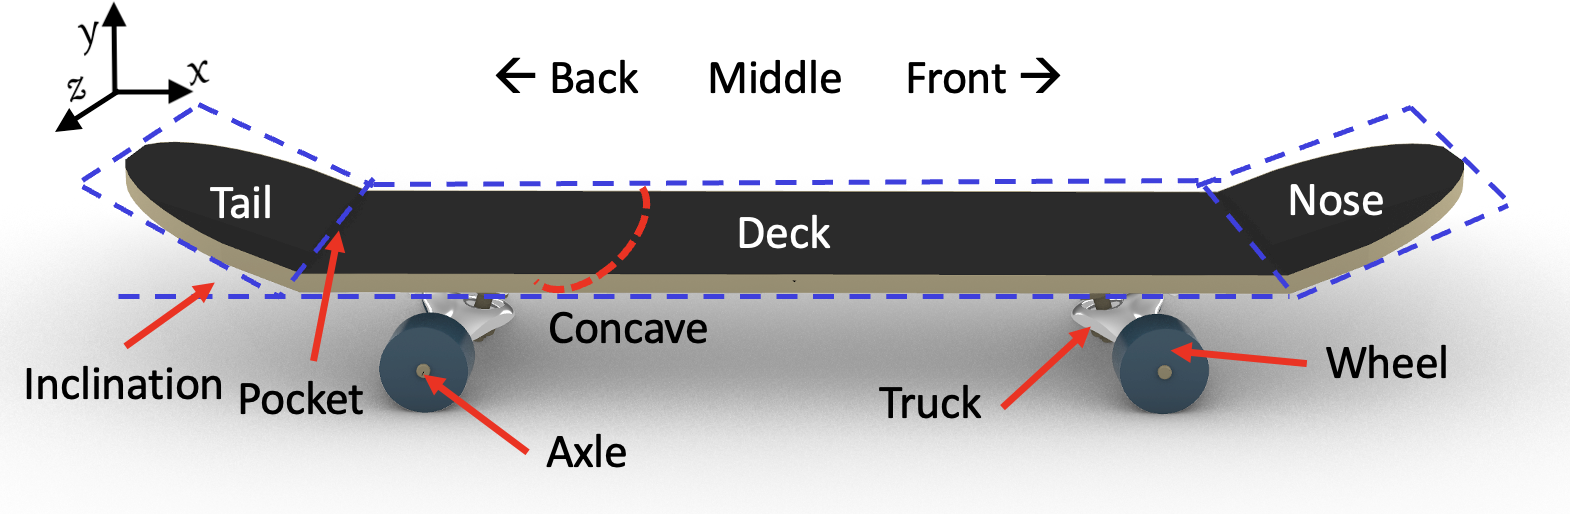
\includegraphics[width=0.5\textwidth]{figure/terminology.png}
\caption[Skateboard terminology]{Skateboard terminology}
\label{f_skateterminology}
\end{figure}

%%%%% END OF HOW TO CHANGE %%%%%%%



\section{Method}
% I have parameterized the geometry and inertia characteristics of a skateboard modeled as a single rigid body with parameters: tail length, tail angle, deck length, truck height, and wheel radius. This is an appropriate parameterization for a skateboard designer because the width of the skateboard is usually chosen by preference. Also, the ollie is a movement that involves rotation in one plane, visible in fig. \ref{f_olliesteps}, which means only the inertia characteristics for this rotation are necessary. 

The chosen method is modeling and optimization to find the optimal skateboard geometry. The hierarchy of the paper will follow these four fundamental steps: 
\begin{enumerate}
    \item Understanding the Mechanics of the ollie through literature and a video analysis
    \item Defining the Optimal Control Problem (OCP) and parameter optimization
    \item Implementing the mechanics into the optimization
    \item Solve the optimization problem for the dimensions of the skateboard for maximum ollie height. 
\end{enumerate}

\subsection{Mechanics of the ollie} \label{ss_mechanics}

%%%%%%%%%%%%%%%% begin figure %%%%%%%%%%%%%%%%%%%
\begin{figure}[b]
\subfloat[Vertical ground reaction force]{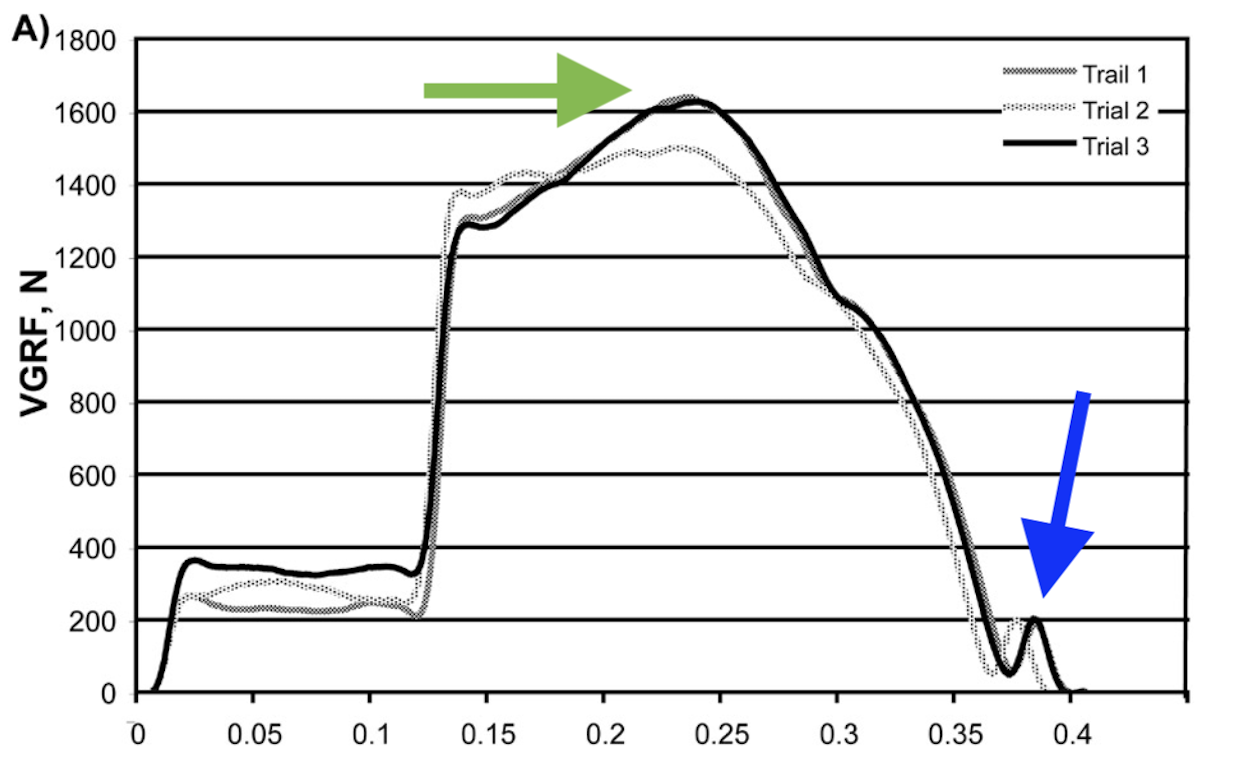
\includegraphics[width=\columnhsize]{figure/GRF1.png}} 

\caption[Ollie vertical ground reaction force]{Take-off ground reaction forces of the ollie. The green arrow is the highest force peak which coincides with the lowest athlete position. After the green arrow the athlete will move upward. The blue arrow is the skateboard hitting the ground \cite{frederick_biomechanics_2006}}
\label{f_GRF}
\end{figure}
%%%%%%%%%%%%%%%% end figure %%%%%%%%%%%%%%%%%%%

The mechanics is analyzed with a slow motion video to note the motion cues during the ollie. These motion cues ($t_1-t_{11}$) are given in figure \ref{f_olliesteps}. Motion cue $t_3$ and $t_4$ show that there is barely contact between the skaters back foot and the tail during impact. Literature supports this phenomenon. In the vertical ground reaction force (VGRF) graph (fig. \ref{f_GRF}(a)) you can see a VGRF that is similar to jumping without a skateboard. The big difference is the final small lump (blue arrow). When the graph is at the green arrow the athletes centre of mass (COM) is at its lowest point and the concentric jumping phase starts. Then when the graph has fallen to almost 0, the skater is weightless and thus airborne. Then due to the rotation of the skateboard the tail hits the ground and causes the lump at the blue arrow. This same tiny peak is found when performing a kick-flip, a similar movement to the ollie but with a body rotation of the skateboard \cite{determan_kinetics_2006}. Other research states that it is a requirement for the ollie to have the foot separated from the tail to perform an ollie \cite{nakashima_simulation_2021}. 

Due to the force normal to the board exerted by the feet together with sliding movement tangential to the surface, friction occurs between the feet and the grip-tape. This is beneficial for ollie height because without friction, the resultant force (fig. \ref{f_olliesteps} $t_4$, green arrow) is directed more vertically down than resultant force in the scenario with friction (\ref{f_olliesteps} $t_5$, blue arrow). A more vertically up resultant force will result in less downward motion while leveling out the skateboard mid air. The higher the coefficient of friction between the foot and the deck, the more up the resultant force will be. That is why grip-tape with rubber soles is the choice of preference among skaters (coefficient of friction of 0.7 or higher \cite{bron_nog_nodate}). 

Furthermore the video shows that the bio mechanical obstruction of the feet cause the skateboard to not go further up. The knees are fully tucked in at the highest point, the skateboard can't go higher through this physical bound. 

A skateboard bends and flexes during the ollie. This study assumes a rigid body model of the skateboard to reduce mathematical complexity.

\subsection{Optimal Control Problem}
The chosen method to solve the optimal control problem is direct collocation. Direct methods are generally best for problems where dynamics and control must be computed to a similar accuracy, and the structure of the control trajectory is not known a priori \cite{kelly_introduction_2017}. Also, the ollie is highly non-linear and complex movement with high dimensionality . With this method it is possible to increase the dimensionality without increasing the difficulty to converge to the solution. The direct method transcribes a continuous problem into a non-linear programming problem (NLP). The software used is PyCollo for , which is direct orthogonal collocation transcription tool for Python \cite{brockie_predictive_nodate}. The dynamics and constraints are enforced over a discretization. The discretization exists of $N$ collocation points. The collocation points are either mesh points or polynomial points, but all collocation points are enforced to the constraints and dynamics. After transcription the problem is passed to the solver IPOPT (Interior Point OPTimizer). When the found IPOPT solution does not meet the error-tolerance set in PyCollo, the discretization is refined and a new iteration is solved in IPOPT. The solution is interpolated using the Legendre-Gauss-Lobatto (LGL) method. The integration scheme is an implicit Runge-Kutta Kth method \cite{brockie_predictive_nodate}. This high order method will have a high accuracy with the disadvantage that all states and constraints need to be differentiable.

The ollie problem is a hybrid problem, meaning that there will be discontinuities in the states. During impact the velocity states change sign instantly causing discontinuities. Discontinuities are per definition not differentiable, this means that in a higher order optimization the discontinuity need to be solved differently. To merge higher order optimization and discontinuities, multi-phase optimization is used. Multi-phase optimization concerns a sequence of continuous-state phases separated by discrete jumps in the states. Multi-phase optimization requires pre-modeled phases which leaves no opportunity for unsought solutions. Though, they are easier to compute and tend to be more accurate \cite{kelly_introduction_2017}. 

\subsection{Parameterization}\label{s_paropt}
Since we want to optimize the input trajectories simulatenously with the
skateboard's physical parameters, we parameterize the dynamics model so that it
it's mass and inertia scale when geometry changes are made.

The most widely used modern skateboard is the Popsicle stick skateboard. We
simplify the Popsicle stick skateboard design for our 2D model and describe it
with ten variables, see Table~\ref{t_variables}. We enforce symmetry, whereas
in reality nose and tail lengths and inclinations vary. We ignore the concavity
present in the deck. The variables colored blue in Figure~\ref{f_11segments}
are optimized and the green variables are set to an industrial standard because
they influence the mass and inertia properties but play little role in the
ollie dynamics.
%
\begin{table}
  \centering
  \begin{tabular}{=l +l +c}
    \rowstyle{\textbf}& Variable & Description \\
    \hline
    \rowstyle{\color{blue}} & $l_{wb}$ & Wheelbase \\
    \rowstyle{\color{blue}} & $l_{d}$ & Deck length \\
    \rowstyle{\color{blue}} & $l_{t}$ & Tail/nose length \\
    \rowstyle{\color{blue}} & $\phi$ & Tail/nose inclination \\
    \rowstyle{\color{blue}} & $h_{tr}$ & Truck height \\
    \rowstyle{\color{blue}} & $r_{w}$ & Wheel radius \\
    \rowstyle{\color{ao}} & $h_d$ & Deck thickness \\
    \rowstyle{\color{ao}} & $d_{tr}$ & Truck width \\
    \rowstyle{\color{ao}} & $d_{d}$ & Deck width \\
    \rowstyle{\color{ao}} & $d_w$ & Wheel width \\
    \rowstyle{\color{orange}} & $d_{com}$ & COM distance from deck \\
  \end{tabular}
  \caption{Variables used to describe skateboard shape (see fig.
    \ref{f_11segments}). Blue parameters are optimized, green parameters are
    set to industrial standard. Orange is a dependent on other variables.}
  \label{t_variables}
\end{table}

%%%%%%%%%%%%%%%% begin figure %%%%%%%%%%%%%%%%%%%
\begin{figure}
  \centerline{
    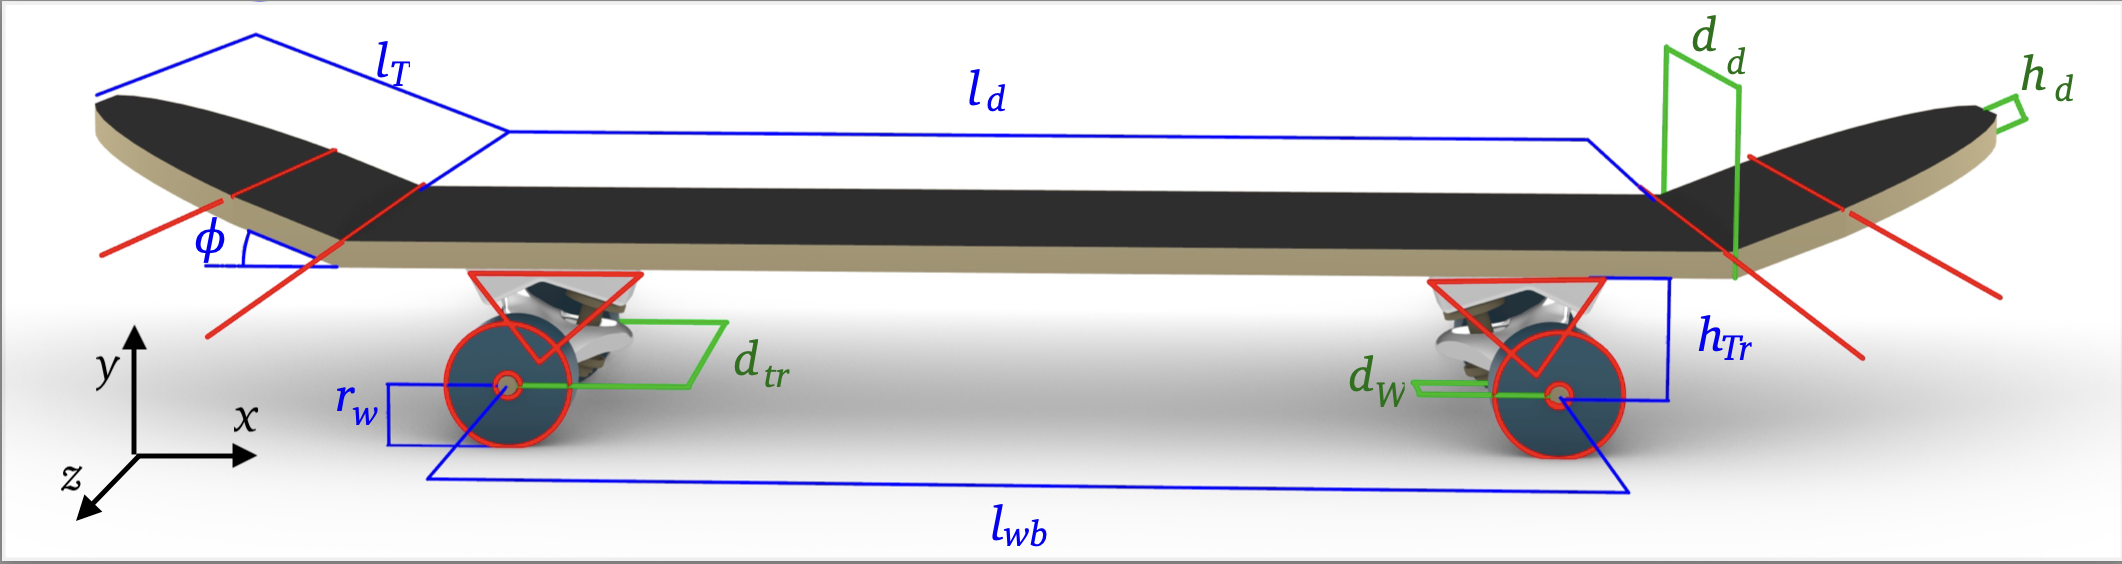
\includegraphics[width=0.5\textwidth,trim={0.1cm 0.1cm 0.1cm 0.05cm},clip]{figure/parameterized.png}
  }
  \caption[11-Segment skateboard model]{Parameterized skateboard. Red lines
    split the skateboard into 11 basic shaped segments for inertia calculation
    (see figure \ref{f_basicshapes})}
\label{f_11segments}
\end{figure}
%%%%%%%%%%%%%%%% end figure %%%%%%%%%%%%%%%%%%%


We developed a mass and inertial model which is a function of the skateboard's
essential geometry, see Figure~\ref{f_11segments}), and material densities
(wood, steel, urethane). The model is made up of eleven basic constant density
shapes shown in Figure~\ref{f_basicshapes}: semi-cylinders, cuboids, cylinders
and triangular prisms.
%
\begin{figure}
  \centering
  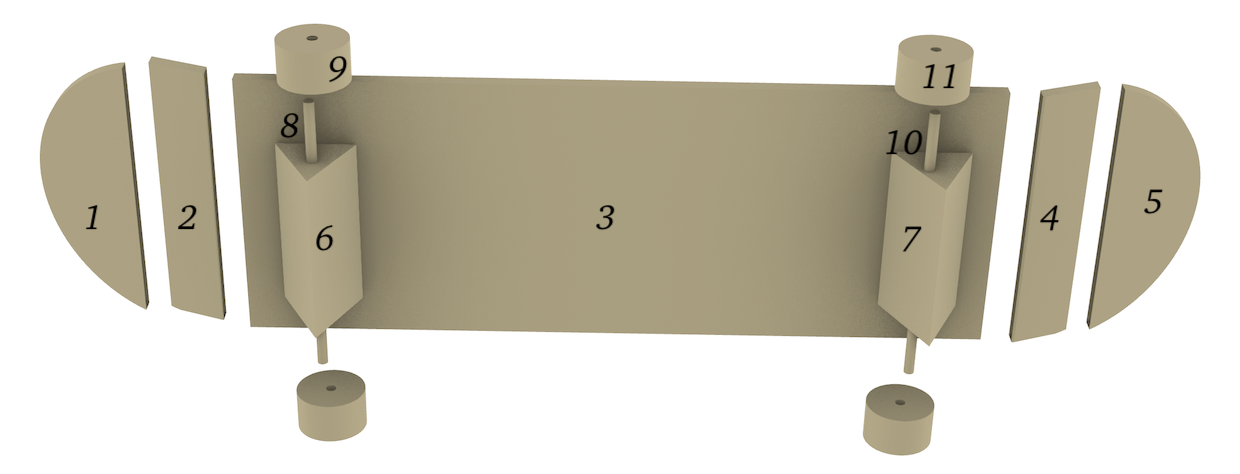
\includegraphics[width = 0.5 \textwidth]{figure/Basicshapes.png}
  \caption[Exploded 11 segment model]{Clarification on the 11 segment model.
    13 shapes are visible, but the wheels are taken as one wider cylinder in
    2D. Sections 1-5 are wood, 6, 7, 8, 10 are steel, and 9, 11 are urethane.}
  \label{f_basicshapes}
\end{figure}

\subsection{Multi-phase Direct Collocation}\label{s_multiphase}
Provided the framework to perform a parameter optimization that scales mass and inertial values accordingly, the ollie optimal control problem is set up next. 

\subsubsection{General formulation}
The multi-phase OCP with phases $p \in [1,2,3]$ involves determining the states $\mathbf{q^{(p)}}$, control $u^{(p)}$, phase initial times $t_0^{(p)}$, phase final times $t_F^{(p)}$, global parameter variables $\sigma$, while maximizing the objective function:
\begin{equation}
    maximize\ \mathcal{J}
\end{equation} 
Subject to the dynamical constraints:
\begin{equation}
\ddot{\mathbf{q}}^{(p)}=\alpha^{(p)}
\end{equation}
with path constraints,
\begin{equation}
        \gamma^{(p)}:\quad \gamma_{min} < ... < \gamma_{max}\\
\end{equation}
and with endpoint constraints:
\begin{equation}
    \beta:\quad \beta_{min} < ... < \beta_{max}
\end{equation}
The ollie OCP will be explained in the order of equations (2-5). Starting with the choice of phases ($^{(p)}$) and objective ($\mathcal{J}$). Then describing the dynamic constraints $\alpha$, consisting of the equations of motion (EOM) for the different phases for the human and the skateboard. Followed by the constraints $\gamma$, where the kinetics and kinematics of the human, and friction are implemented. Then endpoint constraints $\beta$, which contain modeling of impact and the bounding of time. The initial and final state and control values are found in Appendix A and are set to a wide margin. If the margin is not set widely, it will be discussed during these paragraphs. All together, this gives all information necessary to solve the ollie OCP. %Section \ref{s_summary} gives a summary of the implementations before starting the results section.

In section \ref{ss_model} are the geometrical variables described that are optimized. Leading to global optimization parameter variables:
\begin{equation}
\begin{array}{rlrl}
    \sigma_{1} &= l_{wb},\ \sigma_{2} &= l_d,\ \sigma_{3} &= l_t,   \\ 
    \sigma_{4} &= \phi,\ \sigma_{5} &= h_{tr},\  \sigma_{6} &= r_w 
\end{array}
\end{equation}

\subsubsection{Phases and Objective} \label{s_phases}
For the purpose of the optimization this has been simplified to three phases:
\begin{enumerate} \label{n_phases}
    \item Preparation phase 
    \item Upward motion 
    \item Downward motion 
\end{enumerate}
\noindent During the preparation phase the back wheels are in contact with the ground. Between the preparation and upward motion phases, the tail impacts the ground and states will have discontinuities. The dynamics change between the preparation and upward motion phases due to the loss of contact of the back wheels. The dynamics between the Upward and downward motion stay the same. The Upward motion and downward motion are split into two phases because the objective function of the multi-phase optimization needs to be a function of initial or final state variables \cite{brockie_predictive_nodate}. The objective is to ollie as high as possible, now the final state variables of phase two can be used to describe the objective. 

Because a parameter optimization will occur simultaneously with finding the optimal trajectory, the parameters should not be able to influence the objective. To make sure the objective function is independent of the parameter variables, the skateboard is constrained to be level at the highest point and the objective is the middle of a fictional tangent touching lowest point of both wheels. This result in the objective function:

\begin{equation}
    \mathcal{J} = y_s^{(2)}(t_F) + d_{com} - h_{tr} - r_w 
\end{equation}

\noindent Where $y_s^{(2)}(t_F)$ is the final state COM location of the skateboard, $d_{com}$ the skateboards' COM to the deck, $h_{tr}$ the truck height, and $r_w$ is the wheel radius.

\subsubsection{System Dynamics}\label{s_systemdynamics}
\begin{figure}
    \centering
    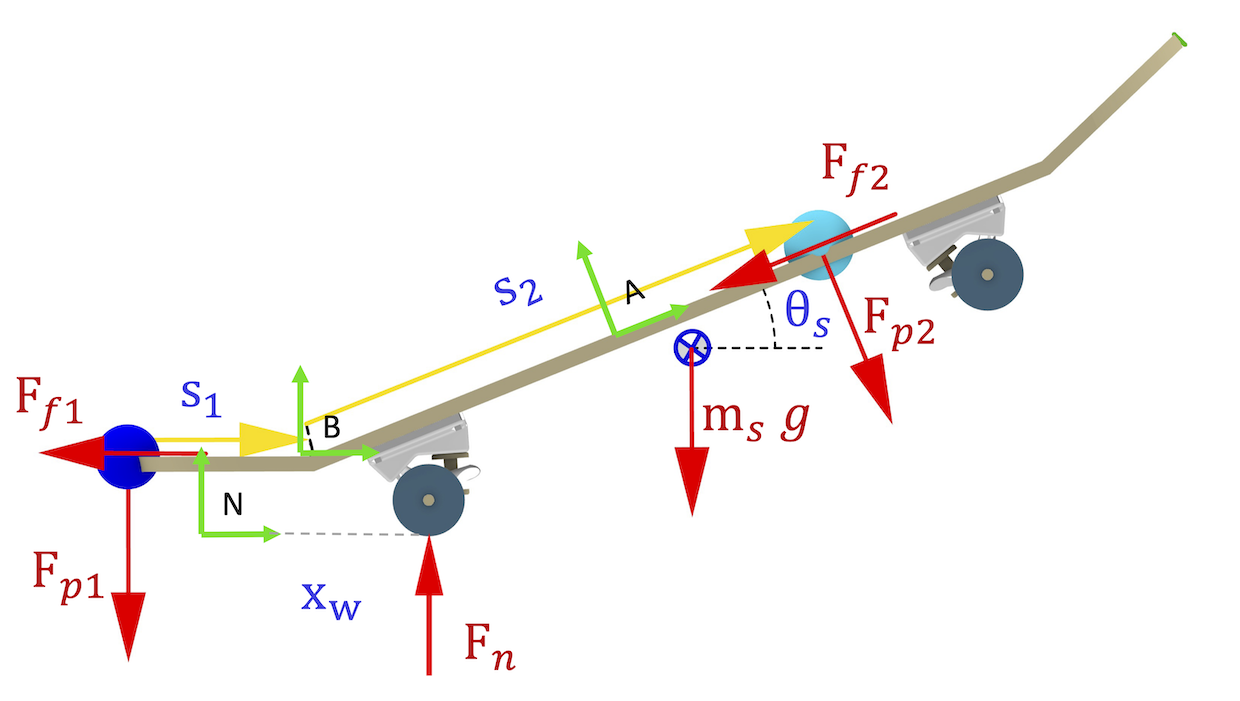
\includegraphics[width = 0.5\textwidth]{figure/FBD_phase1.png}
    \footnotesize\begin{tabular}{|l l|l l|} \hline
    \color{blue}Blue: & State variables &\color{red} Red: & Forces \\ \hline
    \color{cyan}Cyan dot: & Front foot & \color{blue}Blue dot: & Back foot \\ \hline
    \color{yellow}Yellow: & Foot movement & \color{green}Green: & Frames \\ \hline
    \end{tabular}
    \caption[Free body diagram phase 1]{Free body diagram phase 1. The back wheel is now modeled as sliding joint which reduces the degrees of freedom to 2. This is really  similar to the cart-pole problem. The equations are correct as long as the normal force at the wheel is not negative.}
    \label{f_FBDphas1}
\end{figure}

\noindent \; \textbf{Skateboard Equations of Motion - phase 1}\\
The EOMs are derived using SymPy mechanics and symbolic toolbox \cite{meurer_sympy_2017}. The EOM of the skateboard are derived with the TMT method \cite{vallery_heike_advanced_2018}. As stated in section \ref{s_phases}, the dynamics of phase 1 and 2 are different. During phase 1 the EOM are derived with a sliding joint at the back wheel. This is done to eliminate the ground reaction forces from the EOM. The COM coordinates are

\begin{equation}
    \mathbf{x} = [x_s, y_s, \theta_s]^T
\end{equation}

The skateboard when considering the back wheel as a joint can be described by two generalized coordinates $x_w$ (x-location back wheels), and $\theta_s$ (angle w.r.t. ground) as shown in figure \ref{f_FBDphas1}. This is done to eliminate the ground reaction forces. The skateboard has 2 degrees of freedom (DOF), leading to the generalized coordinates:

\begin{equation}
    \mathbf{q} = [x_w, \theta_s]^T
\end{equation}

And the CoM coordinates expressed in the generalized coordinates are:

\begin{equation}
\mathbf{x}=\left[\begin{array}{c}
\frac{l_{w b} \cos \left(\theta_s\right)}{2}+x_w+\left(d_{c o m}-h_{t r}\right) \sin \left(\theta_s\right) \\
\frac{l_{w b} \sin \left(\theta_s\right)}{2}+r_w+\left(h_{t r}-d_{c o m}\right) \cos \left(\theta_s\right) \\
\theta_s
\end{array}\right]
\end{equation}

Differentiating $\mathbf{x}$ once and taking the Jacobian with respect to the velocities gives transformation matrix T:

\begin{equation}
    J_{\dot{\mathbf{x}}}(\mathbf{q}) = \textbf{T} = \left[\begin{array}{c c}
1 & -\frac{l_{w b} \sin \left(\theta_s\right)}{2}+\left(d_{c o m}-h_{t r}\right) \cos \left(\theta_s\right) \\
0 & \frac{l_{w b} \cos \left(\theta_s\right)}{2}+\left(d_{c o m}-h_{t r}\right) \sin \left(\theta_s\right) \\
0 & 1
\end{array}\right]
\end{equation}

Convective terms $\mathbf{g_k}$ are found by taking the Jacobian of $\mathbf{\dot  x}$ with respect to $\mathbf{q}$ and multiplying it by $\mathbf{\dot  q}$ (e.g. $J_{\mathbf{\dot  x}}(\mathbf{q})\cdot \mathbf{\dot  q}$):

\begin{equation}
\mathbf{g_k} = 
\left[\begin{array}{c}
\dot \theta_s^2\left(-\frac{l_{w b} \cos \left(\theta_s\right)}{2}-\left(d_{c o m}-h_{t r}\right) \sin \left(\theta_s\right)\right) \\
\dot \theta_s^2\left(-\frac{l_{w b} \sin \left(\theta_s\right)}{2}+\left(d_{c o m}-h_{t r}\right) \cos \left(\theta_s\right)\right) \\
0
\end{array}\right]
\end{equation}
Two sets of bound vectors are equivalent when they equal resultants and equal moments about any point \cite{moore_force_nodate}. This means that all the forces acting on the skateboard can be described by resultant forces on and moments to the COM. The forces acting on the skateboard are the frictional ($F_{f1,2}$) and normal forces $F_{p1,2}$ from the front and the back foot. The back and front feet are indicated with a blue and cyan dot and are defined on the skateboard with variables $s_1$ and $s_2$ respectively. The perpendicular forces are bound positively such that the feet can never pull on the board. The moments caused by the back and front foot about the COM are $Mc_{bf}, Mc_{ff}$ respectively. Thus the CoM-applied forces and torques $\mathbf{F_{a}}$ are:
 
\begin{equation}\label{e_Fi}
\begin{array}{c}
    \mathbf{F_{a}}= \left[\begin{array}{l}
-F_{p 1} \sin \left(\phi-\theta_s\right)+F_{p 2} \sin \left(\theta_s\right)- \\ \ F_{w 1} \cos \left(\phi-\theta_s\right)-F_{w 2} \cos \left(\theta_s\right) \\ \\
-F_{p 1} \cos \left(\phi-\theta_s\right)-F_{p 2} \cos \left(\theta_s\right)+ \\ \ F_{w 1} \sin \left(\phi-\theta_s\right)-F_{w 2} \sin \left(\theta_s\right)-g m_s \\ \\
Mc_{bf} + Mc_{ff}
\end{array}\right] 
\\ \\
Mc_{bf} = -F_{p 1} (-d_{\text {com }} \sin (\phi)-\frac{l_d \cos (\phi)}{2}-l_t+s_1)+ \\ \ F_{w 1}(d_{c o m} \cos (\phi)-\frac{l_d \sin (\phi)}{2})
\\ \\
Mc_{ff} = -F_{p 2}\left(-\frac{l_d}{2}+\mathrm{s}_2(t)\right)+F_{w 2} \ d_{c o m}
\end{array}
\end{equation}  

The skateboards' mass matrix $\mathbf{M_s} = diag(m_s,m_s,I_s)$ together with the transformed CoM applied coordinates form the EOM of phase 1:
\begin{equation} \label{e_eoma}
    \mathbf{T}^T \mathbf{M_s} \mathbf{T} \cdot \left[\begin{array}{c}
         \ddot x_w  \\
         \ddot \theta_s 
    \end{array}\right] = \mathbf{T}^T (\mathbf{F_a} - \mathbf{M_s} \cdot \mathbf{g_k})
\end{equation}
Rewriting the EoM gives two dynamical constraints valid for phase 1:

\begin{equation}
    \alpha_{1,2}^{(1)} =   \left(\mathbf{T}^T \mathbf{M_s} \mathbf{T} \cdot  \mathbf{T}^T\right)^{-1} (\mathbf{F_a} - \mathbf{M_s} \cdot \mathbf{g_k})
\end{equation}

\begin{figure}
    \centering
    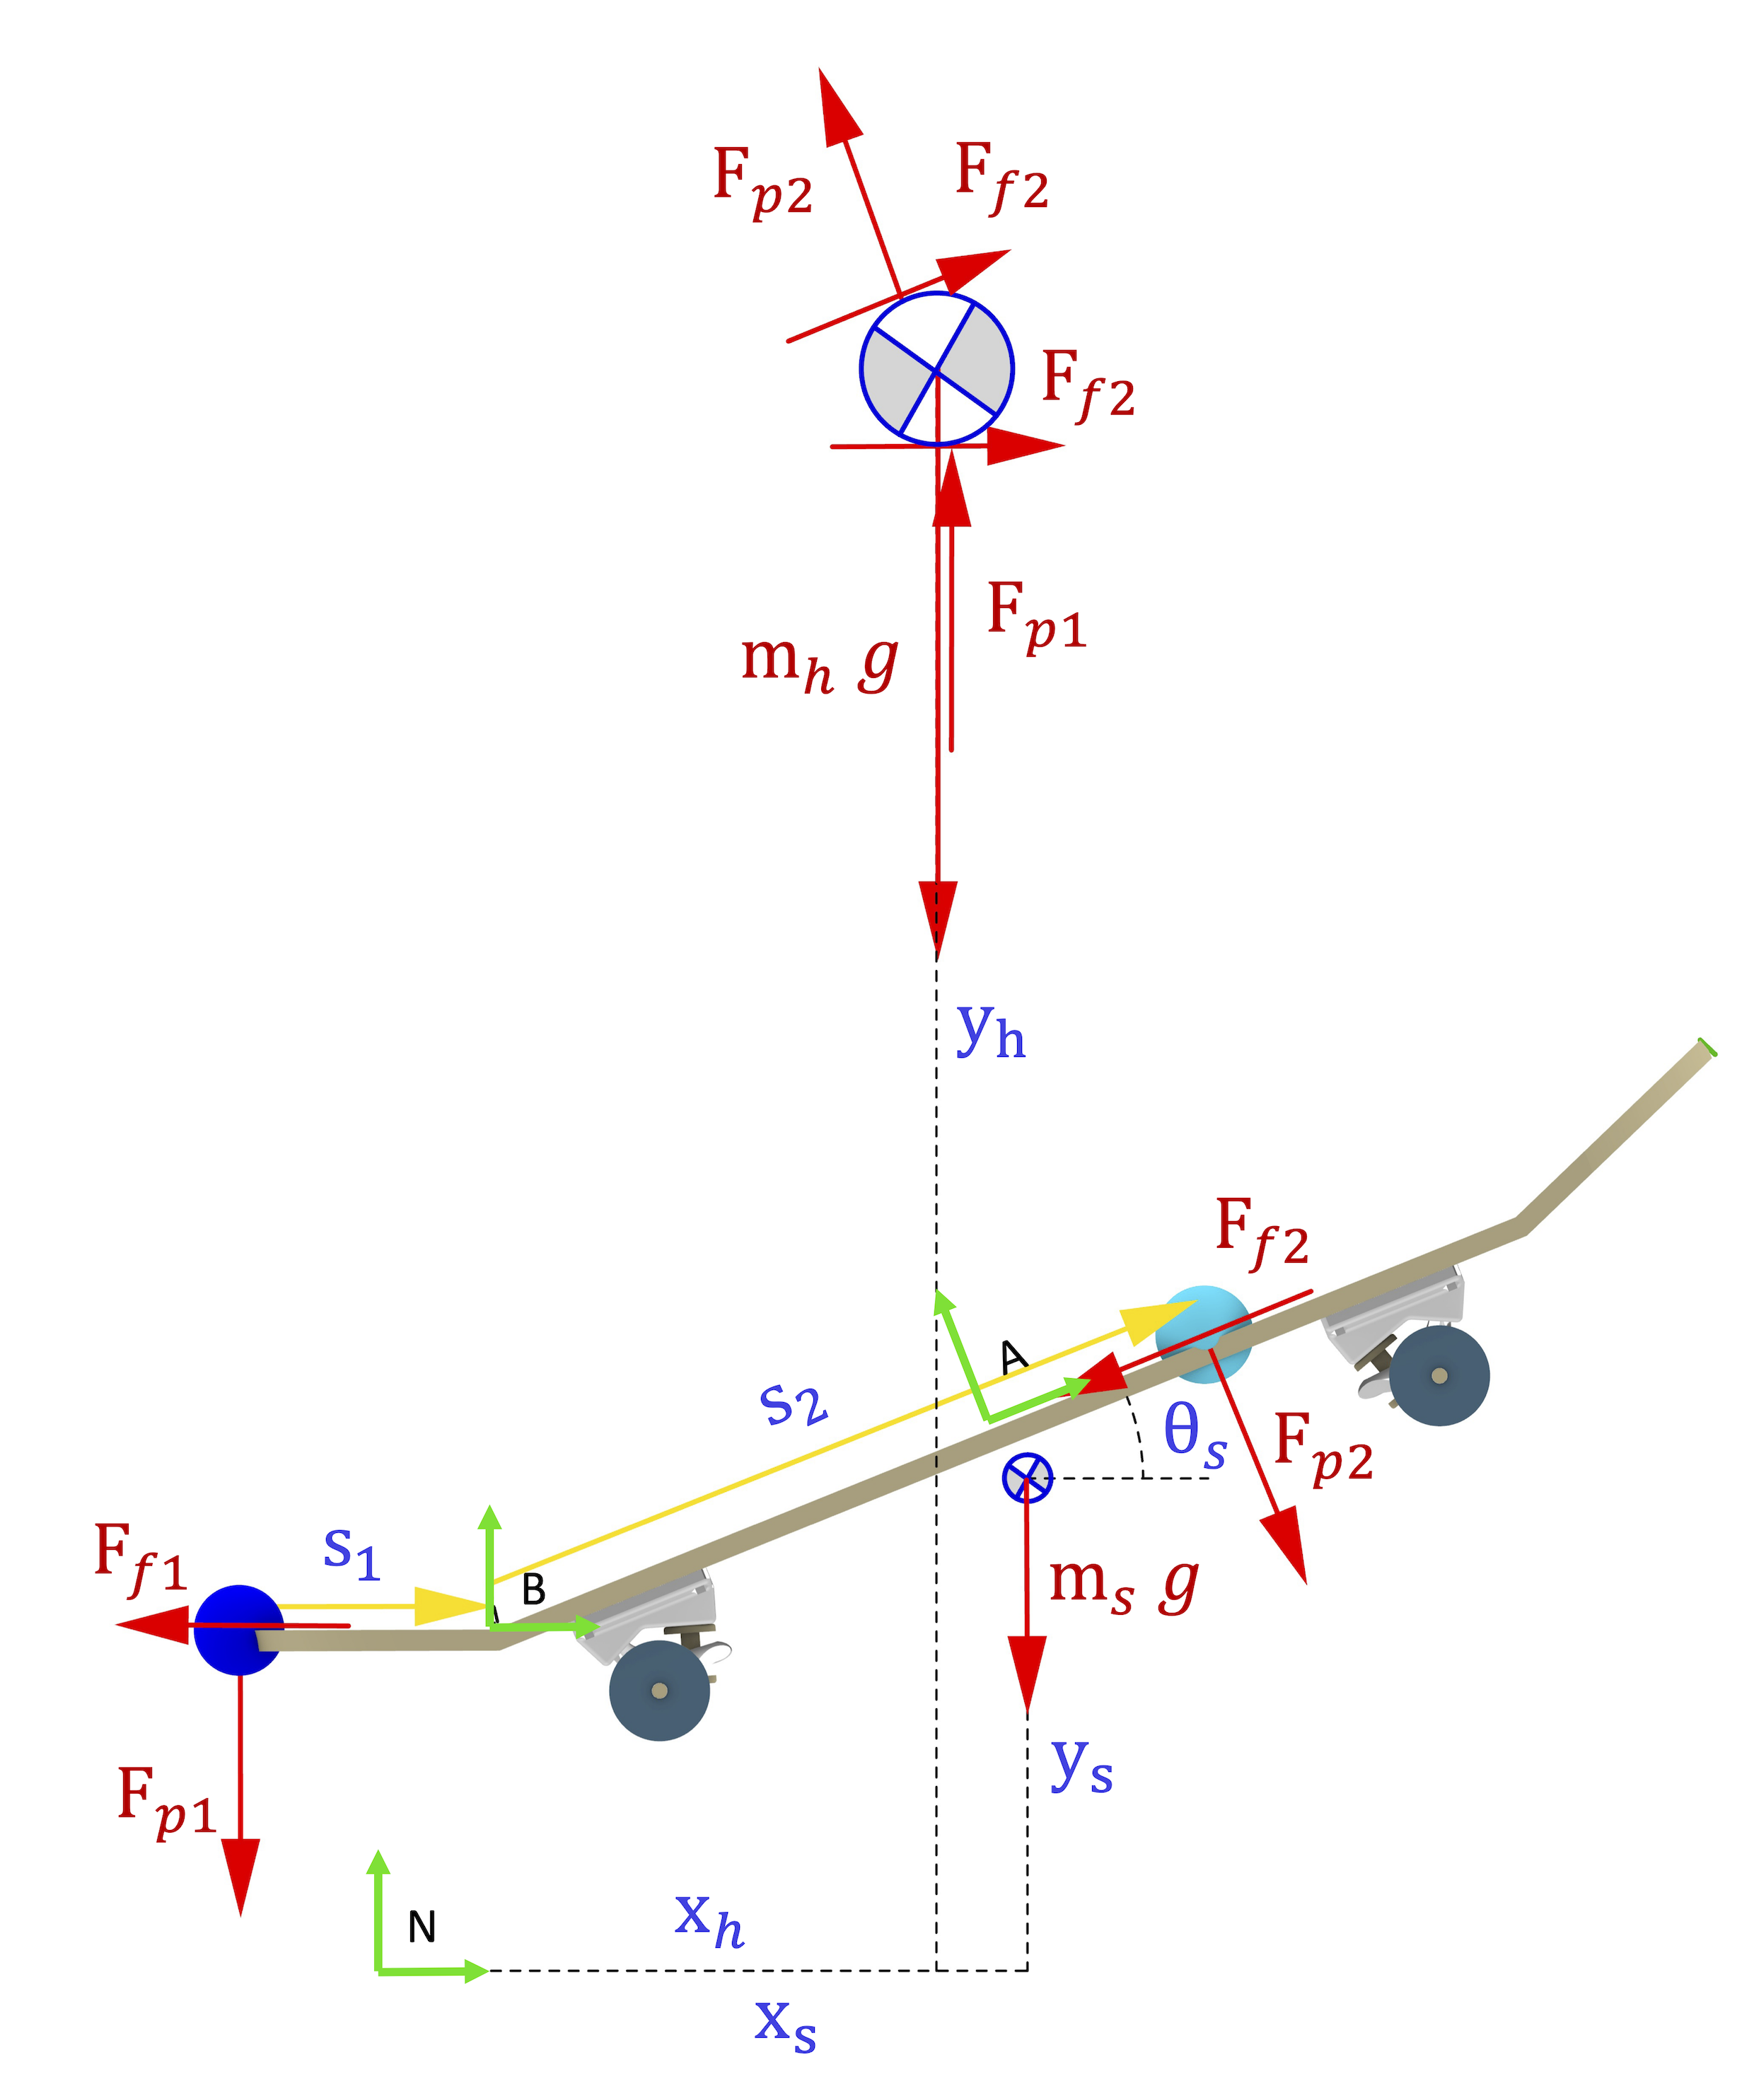
\includegraphics[width=0.45\textwidth]{figure/FBD_skater_feet.png}
    \footnotesize\begin{tabular}{|l l|l l|} \hline
    \color{blue}Blue: & State variables &\color{red} Red: & Forces \\ \hline
    \color{cyan}Cyan dot: & Front foot & \color{blue}Blue dot: & Back foot \\ \hline
    \color{yellow}Yellow: & Foot movement & \color{green}Green: & Frames \\ \hline
    \end{tabular}
    \caption[Free Body Diagrams phase 2 and 3]{Free body diagrams of human and skateboard for phase 1. N Frame is the inertial frame, A and B are body fixed frames. Forces are equal and opposite acting between the feet and human COM.}
    \label{f_FBD}
\end{figure}

\textbf{Human Equations of Motion} \\
\noindent The skateboard is controlled by a mass point on top of the skateboard representing the human. The interaction between the mass point and the skateboard are simulated with equal and opposite forces acting between the massless feet and the CoM of the human (see fig. \ref{f_FBD}). The simplification ignores many body segments. Which means this model is not representable in terms of metabolic leg power. Only the mechanical power output can be estimated with this model \cite{van_der_kruk_power_2018,morin_biomechanics_2018}. With this approximation, inertia of the humans' body and segments is neglected. This is reasonable because during the ollie, the human rotates minimally on top of the skateboard (see figure \ref{f_olliesteps}). 

The human has two degrees of freedom; $x_h$, and $y_h$. The EOMs of the human are found with the Newtons equations of motion:

\begin{equation}\label{e_newton}
\begin{array}{c}
        m_s \cdot \ddot x_s = \sum F_x  \\
        m_s \cdot \ddot y_s = \sum F_y  \\
    \end{array}
\end{equation}

\noindent Forces acting on the human are:

\begin{equation} \label{e_humanforce}
\begin{array}{cc}
      \mathbf{F_{bf}} = F_{p1} \cdot \mathbf{\hat b_y} + F_{f1} \cdot \mathbf{\hat b_x}\\
      \mathbf{F_{ff}} = F_{p2} \cdot \mathbf{\hat a_y} + F_{f2} \cdot \mathbf{\hat a_x}\\
      \mathbf{F_h}    = \mathbf{F_{bf}} + \mathbf{F_{ff}}
\end{array}
\end{equation}

\noindent Where $\mathbf{F_{bf}}$, and  $\mathbf{F_{ff}}$ are the back foot forces, and front foot forces respectively. Combining equation \ref{e_newton} and \ref{e_humanforce} expressed in the inertial frame N gives the EoM for the human for all three phases:

\begin{equation}
    \left[\begin{array}{cc}
        m_h & 0 \\
        0 & m_h \\
    \end{array}\right] \cdot \left[\begin{array}{c}
         \ddot x_h  \\
         \ddot y_h \\
    \end{array}\right]=\left[\begin{array}{c}
        \mathbf{F_h}\cdot \mathbf{\hat n_x}  \\
        \mathbf{F_h}\cdot \mathbf{\hat n_y}\\
    \end{array}\right]
\end{equation}

Which lead to two dynamic constraints for all three phases:

\begin{equation}
\begin{split}
        \alpha_{3}^{(1,2,3)} = \frac{\mathbf{F_h}\cdot \mathbf{\hat n_x}}{m_h}\\
        \alpha_{4}^{(1,2,3)} = \frac{\mathbf{F_h}\cdot \mathbf{\hat n_y}}{m_h}
\end{split}
\end{equation}

\textbf{Flight Equations of Motion - phases 2 and 3} \\
\noindent The EoM for phases 2 and 3 for the skateboard are without ground contact. The skateboard is now a free-floating body in space with 3 DOF resulting in:

\begin{equation}\label{e_eomb}
\mathbf{M_s} \cdot \left[\begin{array}{c}
         \ddot x_s  \\
         \ddot y_s \\
         \ddot \theta_s 
    \end{array}\right] =  \mathbf{F_a}
\end{equation}

This leads to the last two dynamic constraints valid for phase 2, and 3:

\begin{equation}
    \alpha_{5,6}^{(2,3)} = (\mathbf{M_s})^{-1}\mathbf{F_a}
\end{equation}

%%%%%%%%%%%%%%%% begin figure %%%%%%%%%%%%%%%%%%%
\begin{figure}[b]%
    \centering
    \subfloat[\centering 45.5" world record ollie. $^{1}$  ]{{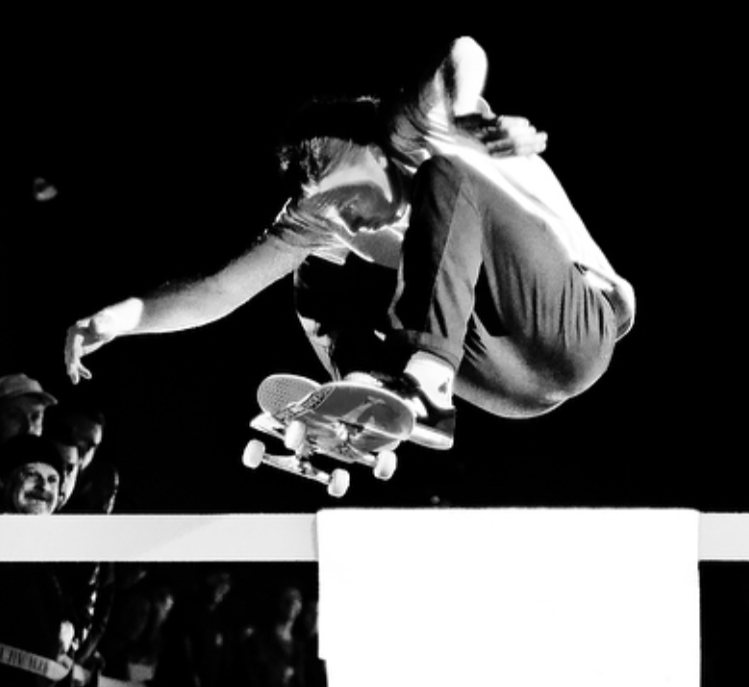
\includegraphics[width=0.2\textwidth]{figure/JakeHayes.png} }}%
    \quad
    \subfloat[\centering Yeadon model in same configuration]{{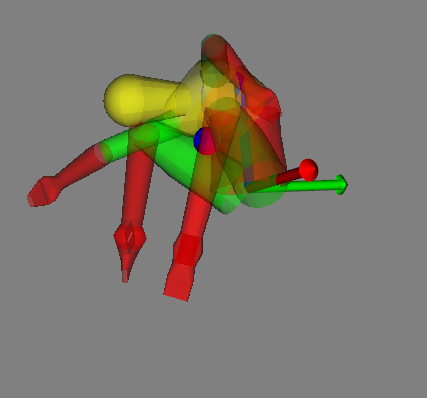
\includegraphics[width=0.2\textwidth]{figure/JakeHayesYeadon.png} }}%
    \caption{Reconstruction of world record ollie} 
    \label{fig:f_record}
    \centering \footnotesize \url{https://theberrics.com/world-record-ollie-footage}$^{1}$%
\end{figure}
%%%%%%%%%%%%%%%% end figure %%%%%%%%%%%%%%%%%%%

\subsubsection{Constraints}
\quad \textbf{Human}\\
The human is simplified as a point mass which reduces complexity for the optimization but sacrifices the reality. To make sure the human as a point mass still gives the output of a more complex model, the kinetics and kinematics will be constrained. 

\textit{Kinematics} \\
The kinematics of the human controller are bound by the musculoskeletal restrictions of the human body. The musculoskeletal restricions are difficult to comprise in a point mass model. The first restriction is that the feet can only be within a certain distance of the human COM. This is not simply the leg length, because the COM location of the human will change when the legs are moved. The maximum and minimum feet location with respect to the COM of the human are found with Yeadon, a package for Python to configure a humanoid to a position and find distances between points \cite{yeadon_simulation_1990}. The model is set to a 1.80[m] tall human and is matched to a picture of the world record ollie of Jake Hayes. The reconstruction is seen in fig.\ref{fig:f_record}. This leads to the first two constraint:


\begin{equation}\label{e_yeadon}
\begin{array}{c}
    \gamma_{1}^{(2,3)}:\quad  0.466 < y_h - \mathbf{r_{comH \mathbin{/} bf}} \cdot \mathbf{\hat n_y} < 1.13 \\ 
    \gamma_{2}^{(2,3)}:\quad  0.466 < y_h - \mathbf{r_{comH \mathbin{/} ff}} \cdot \mathbf{\hat n_y} < 1.13 
\end{array}
\end{equation}

These constraints describe that the vertical ($\mathbf{ \hat n_y}$) distance between the feet and the COM can never be outside of the given bounds. This constraint will not exceed musculoskeletal limits if the feet do not separate an an extreme distance (split). To make sure this behaviour does not happen, another constraint is implemented that the feet should never be separated more from each other than within a reasonable operating distance.

\begin{equation}
        \gamma_{3}^{(1,2,3)}:\quad   0.1 < \vert \mathbf{r_{bf/ff}} \vert < 1
\end{equation}

The skater should not leave the board in horizontal direction either. This gives the next constraint:
\begin{equation}
    \gamma_4^{(1,2,3)}:\quad  -0.3 < x_h - \mathbf{r_{comS\mathbin{/}comH}}\cdot \mathbf{\hat n_x} < 0.3
\end{equation}

To make sure the feet never leave the skateboard, $s_1$ and $s_2$ are positively bound from the end of the tail and the left pocket of the deck respectively (see fig \ref{f_FBD}):
\begin{equation}
\begin{array}{c}
    \gamma_{5}^{(1,2,3)}:\quad  0 < s_1-l_t < \infty  \\
    \gamma_{6}^{(1,2,3)}:\quad  0 < s_2-l_d < \infty  \\
\end{array}
\end{equation}
The feet can still be in a no contact scenario as seen in section \ref{ss_mechanics}. This is simulated by when zero force is exerted. 

\textit{Kinetics} \\
The kinetics of the human are bound to the characteristics of the countermovement jump (CMJ) during the first phase of the ollie. The CMJ motion is chosen because, 76.3\% of the variance in the performance of the ollie maneuver can be explained by the CMJ (CMJ) \cite{candotti_lower_2012}. The CMJ is reported to have good reliability and is a strong assessment of lower-body mechanical power \cite{barker_relationships_2018}. During a vertical jump, joint torques, knee extensor force, hip abduction forces all map to one output variable: the ground reaction force (GRF). Bounding the GRF is the only sensible way to capture the kinetics of a human jumper for a point mass model is the ground reaction force, because contributions of individual segments can only be bound with more complex models. Hence, the GRF of the CMJ is used to realize a realistic COM human jumper model. In figure \ref{f_cmj} a typical ground reaction force for a CMJ is shown. By constraining the vertical rate of force development (RFD) ($dF/dt$, slope in figure \ref{f_cmj}), the maximum force $F_{max}$, maximum displacement $\Delta s$, and maximum mechanical power $P$, the total mechanical output of the legs is constrained for a simple point mass model. By constraining the RFD, the shortening or lengthening cycle is simulated. The maximum force will make sure the force does not exceed the maximum capabilities. By constraining the power, given a constrained force, the maximum velocity is also constrained due to $P = F v_{rel}$.
Due to a constrained maximum distance($ \Delta s $) the force can work over, the work done is also constrained due to $ W = F ds $, given a constrained force. The data for the RFD, $ F_{max} $, $ \Delta s $, $ P $ is taken from a Division-I male, soccer players with a mean height of 179.5[cm], weight of 75.5[kg], and age of 19.65 years \cite{barker_relationships_2018}. $ \Delta s $ and $ P $ are calculated in the paper with a point mass approximation which is important to map to the optimization properly. The data was measured for two legs simultaneously, which is unfortunate for the optimization since the two legs can work separately, which might lead to different kinetic data. Though, the constraints are set on the sum of the forces and the forces separately due to the possibility of out of phase pushing and pulling which could result in a combined satisfaction of the constraint but individual legs could exceed the physical limitations. The maximum distance is constraint implemented similar to equation \ref{e_yeadon} with the same upper bound:

\begin{equation}
\begin{split}
        \gamma_{7}^{(2,3)}:& \quad  1.13-\Delta s < y_h - \mathbf{r_{comH \mathbin{/} bf}} \cdot \mathbf{\hat n_y} < 1.13 \\ 
      \gamma_{8}^{(2,3)}:& \quad  1.13-\Delta s < y_h - \mathbf{r_{comH \mathbin{/} ff}} \cdot \mathbf{\hat n_y} < 1.13 
      \end{split}
\end{equation}

\begin{figure}
    \centering
    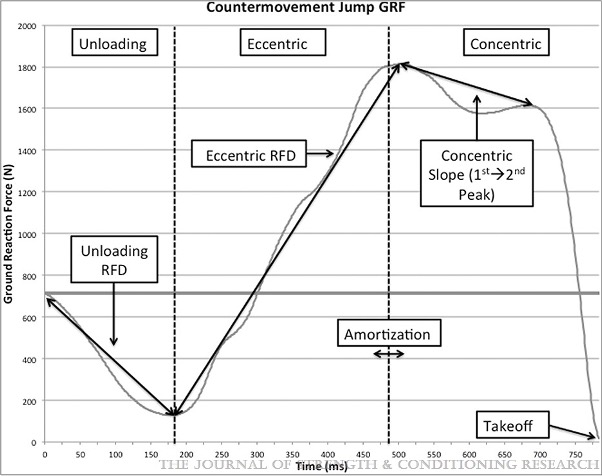
\includegraphics[width=0.4\textwidth]{figure/countermovementjumpRFD.jpg}
    \caption[Ground reaction force of CMJ]{Phases during CMJ. During unloading, the human lowers their COM quickly. During the eccentric phase, the gained downward velocity during the unloading phase is braked until the lowest point is reached which is at the amortization. During the concentric phase the legs are stretched out and upward speed is gained until the take-off. At take-off the vertical speed is maximal.}
    \centering \footnotesize Source: \cite{barker_relationships_2018}%
    \label{f_cmj}
\end{figure}

\noindent The maximum force constraints are set at the sum of all vertical forces $\mathbf{F_h}\cdot \mathbf{\hat n_y}$, and to the vertical components of the back and front feet ($\mathbf{F_{bf}}\cdot \mathbf{\hat n_y}, \mathbf{F_{ff}}\cdot \mathbf{\hat n_y}$)

\begin{equation}
\begin{array}{c}
    \gamma_{9}^{(1,2,3)}:\quad  -32.61 m_h < \mathbf{F_h}\cdot \mathbf{\hat n_y} < 32.61 m_h   \\
    \gamma_{10}^{(1,2,3)}:\quad  -32.61 m_h < \mathbf{F_{bf}}\cdot \mathbf{\hat n_y} < 32.61 m_h \\
    \gamma_{11}^{(1,2,3)}:\quad  -32.61 m_h < \mathbf{F_{ff}}\cdot \mathbf{\hat n_y} < 32.61 m_h \\
\end{array}
\end{equation}

The unloading RFD ($-41.8 m_h$) and eccentric RFD ($196.41 m_h$) are implemented in constraint:

\begin{equation}
    \gamma_{12}^{(1)}: \quad  -41.8 m_h < \dot{\mathbf{F_h}} \cdot \mathbf{\hat n_y} < 196.41 m_h  
\end{equation}

The power is found per leg by calculating the dot product between relative velocity between the foot and the human COM and the resultant force acting on the foot. 

\begin{equation}\label{e_power}
    \begin{array}{c}
         P_{bf} = \mathbf{\dot r}_{comH/bf} \cdot \mathbf{F_bf}  \\
         P_{ff} = \mathbf{\dot r}_{comH/ff} \cdot \mathbf{F_bf}  \\
    \end{array}
\end{equation}

Just like the maximum force constraints, the legs can work out of phase (one leg negative work, one leg positive). To avoid that the limits are exceeded the power needs to be bound absolutely. Absolute values are not feasible in higher order optimization problems \cite{kelly_introduction_2017}. Absolute bound can be made with three bounds instead:

\begin{equation}
    \begin{array}{c}
         \gamma_{13}^{(1)}:\quad  -54.62 m_h < P_{bf} + P_{ff} < 54.62 m_h  \\
         \gamma_{14}^{(1)}:\quad  -54.62 m_h < P_{bf} - P_{ff} < 54.62 m_h  \\
         \gamma_{15}^{(1)}:\quad  -54.62 m_h < P_{ff} - P_{bf} < 54.62 m_h  \\
    \end{array}
\end{equation}

The horizontal ($\mathbf{\hat n_x}$) direction forces are now unconstrained. The data in from the CMJ paper does not include any horizontal forces. Since the body of the human does not rotate during the jump, the horizontal forces are approximated with maximum abduction force. The maximum abduction force is obtained by pushing sideways against a scale whilst standing up-straight. This maximum force bound is not very accurate, but the power of abduction force is captured in the power calculation in equation \ref{e_power}. This leads to a reliable abduction force approximation. With the constraints:

\begin{equation}
    \begin{array}{c}
         \gamma_{16}^{(1,2,3)}:\quad  -200 < \mathbf{F_{ff}}\cdot \mathbf{\hat n_x} < 200  \\
         \gamma_{17}^{(1,2,3)}: \quad -200 < \mathbf{F_{ff}}\cdot \mathbf{\hat n_x} < 200 \\ 
    \end{array}
\end{equation}

Only the maximum force constraints $\gamma_{11-13}$ and $\gamma_{18-19}$ apply to all phases. The CMJ constraints are only applied to the first phase, since phase 1 concerns the CMJ movement. 

\textbf{Friction}\\
According to section \ref{ss_mechanics} the feet are sliding along the griptape
to level the skateboard out and drag the skateboard up during the preparation
phase 1, and upward motion phase 2. Static and dynamic friction is are used to
describe this phenomena. The method to implement these in the optimization is a
simplification to the frictional contact implicit optimization called the
relaxed formulation by Patel et al. \cite{patel_contact-implicit_2019}. This
method is able to have unplanned discontinuous frictional contact with direct
collocation without a hybrid method. Usually this would be considered
impossible since direct collocation enforces the dynamics and constraints over
a continuous domain, where discontinuities in the system dynamics usually lead
to infeasibility \cite{kelly_transcription_2017}. The downside is that with
this method it is difficult to converge to a feasible solution without a proper
initial guess and the computation time is rather high
\cite{shield_contact-implicit_2022,patel_contact-implicit_2019}. I have found a
way to simplify this method, which represents a contact implicit frictional
contact that solves optimally under 2 minutes without initial guess. To explain
the simplifications and for the sake of clarity, I will first explain the
impact method of Patel et al..

The relaxed formulation is shown in figure \ref{f_relaxed}. It implements a
contact constraint that will look one time-step ahead to be able to initiate a
contact force before impact. Let $C_c(\mathbf{q})$ be the relative distance
between the two bodies that impact, and let the normal force $F_n$ be a control
variable. The following constraints will ensure that only when the next time
step is in contact ($C_c(\mathbf{q}(t+1)$) the normal force $F_n > 0$ when
there is no contact at the next time step, $F_n$ must be zero:
%
\begin{equation}\label{e_patelimpact}
    F_n\ C_c(\mathbf{q}(t+1) = 0,\quad C_c(\mathbf{q}) \geq 0,\quad F_n \geq 0
\end{equation}

This result of this formulation is shown graphically in figure
\ref{f_discontinuities}. When constraining an optimization problem likewise,
the solver will find the normal forces needed to comply to the non penetration
constraint $C_c(\mathbf{q}) \geq 0$. This method has been used in the
optimization of an ollie. Though the initial guess needed to be similar to the
solution to find feasible solutions. The model with a full body human operator
took 43 minutes to solve \cite{shield_contact-implicit_2022}.

To simplify the model I excluded this impact formulation, because I assume that
the feet are always located on the skateboard, but can be out of contact by
exerting zero force. In this case, where the human is not modeled with multiple
segments but as a point mass, it is possible to exclude equation
\ref{e_patelimpact}. By setting the normal forces of the feet $F_{p1},F_{p2}$
as control variables. The foot location is also regulated by a control
variables. The acceleration is controlled instead of the foot location itself
to still have smooth realistic foot trajectories. Resulting in the control
variables:
%
\begin{equation}
    \mathbf{u}^{(1,2,3)} = [F_{p1},F_{p2},\ddot s_1, \ddot s_2]    
\end{equation}

Now that the difficult to solve contact formulation by Patel in equation
\ref{e_patelimpact} is replaced by a simplified formulation, I will continue
with the friction model that is used in this optimization.  Friction is present
during the ollie when sliding the foot along grip-tape, when rolling, and when
the tail hits the ground if the tail has a relative velocity tangential to the
impact surface. Friction is a highly non-linear and discontinuous phenomenon.
In general the dominant friction components that have been modeled include
static friction (A force that opposes the input force at zero velocity),
Coulomb friction (constant motion opposing force at non-zero velocity), viscous
friction (when fluid exists between the contact surfaces), and the Stribeck
effect (a speed dependent friction) \cite{makkar_new_2005}. 

%When modeling friction continuously, pure static friction does not exist since at zero velocity the friction function will be zero as well due to symmetry. 
Friction can only exist during contact. The friction is solved with a set of
constraints. The first step to implement this friction is to create slack
variables that divide the friction forces as described in the system dynamics
$F_{f1},F_{f2}$ into a positive and negative components. For simplicity reasons
I will only derive the friction of the back foot along the skateboard. The
front foot friction is obtained by exactly the same process. By replacing $_1$
to $_2$ in the following equations, the front foot friction is also realized

\begin{equation} \label{e_plusminfric}
   F_{f1} = F_{f1}^+ - F_{f1}^-
\end{equation}

As described in section \ref{s_systemdynamics}, the forces perpendicular to the
skateboard are positive definite such that the force can never pull on the
skateboard. Now the created slack variables also need to be positive definite:

\begin{equation}
    F_{p1} \geq 0,\quad F_{f1}^+ \geq 0,\quad F_{f1}^- \geq 0
\end{equation}

Static and dynamic friction is bound by the friction cone shown in figure
\ref{f_frictioncone}. The magnitude of dynamic friction is $F_{p1}\ \mu$ with a
direction opposed to the relative sliding velocity (see figure
\ref{f_frictioncone}. The static friction is bound by the yellow surface of the
friction cone in fig. \ref{f_frictioncone} and is only possible when the feet
are not sliding. To realize this, another slack variable $\psi$ is introduced
which represents the magnitude of the relative velocity $\dot s_1$ between the
foot and the skateboard.

\begin{equation}
\begin{split}
    \gamma_{18}^{(1,2,3)}: \quad & \psi_1 + \dot s_1  \geq 0 \\
    \gamma_{19}^{(1,2,3)}: \quad & \psi_1 - \dot s_1  \geq 0 \\
\end{split}
\end{equation}

Now static friction can be implemented with a set of constraints:

\begin{equation}
\begin{split}\label{e_frictioncontrol}
       \gamma_{20}^{(1,2,3)}: \quad & \mu F_{p1} - F_{f1}^+ - F_{f1}^- \geq 0 \\
       \gamma_{21}^{(1,2,3)}: \quad & (\mu F_{p1} - F_{f1}^+ - F_{f1}^-)\ \psi_1  = 0
\end{split}
\end{equation}

The first constraint assures that the positive or negative component of the
friction is always smaller than $\mu F_{p1}$. The second constraint ensures
that when the foot slides ($\psi_1 \not = 0$),  the sum of the positive and
negative friction components equal $\mu F_{p1}$. It is important that when
sliding in positive direction, the negative friction component $F_{f1}^-$
should equal $\mu F_{p1}$ and $F_{f1}^+=0$ and vice versa. This is realized
with the following constraints:

\begin{equation}
\begin{split}
    \gamma_{22}^{(1,2,3)}: \quad & F_{f1}^+ (\psi_1 + \dot s_1)  = 0 \\
    \gamma_{23}^{(1,2,3)}: \quad & F_{f1}^- (\psi_1 - \dot s_1)  = 0
\end{split}
\end{equation}

This type of constraint ($A\cdot B = 0$) has three possible solutions $A= 0,\
B=0,\ or\ A,B = 0$. By filling in a numerical example, the desired behaviour is
shown. For example looking at the first constraint, when $\dot s_1 = -1$, then
$\psi_1 + \dot s =  0$ and $F_{f1}^+$ can be a positive number. Then looking at
the second constraint, when $\dot s = -1$, then $\psi - \dot s = 2$ and
$F_{f1}^- = 0$. Combining this with the second equation in equation
\ref{e_frictioncontrol} gives: $(\mu F_{p1} - F_{f1}^+ - 0) \cdot 0 = 0$, which
results in $F_{f1}^+ = \mu F_{p1}$. This is exactly what it should be given a
negative relative sliding velocity. The friction for the front foot will be
another six constraints: $\gamma_{24-30}^{(1,2,3)}$

\subsubsection{Endpoint constraints} \label{p_endpoints}
To fully describe the ollie optimization problem, all phases need to be glued together. In the multi-phase optimization scheme all initial and final time variables are treated as separate variables. By constraining the corresponding variables between the phases, the variables can be treated as one variable over all three phases.

\textbf{Impact}\\
Just before the skateboard is airborne, the tail hits the ground. During this collision the ground exerts a normal linear impulse normal. The method used\cite{vallery_heike_advanced_2018} is based on the Newton impact law. The Newton impact law rewritten in terms of the optimization states is:

\begin{equation}\label{e_newtonimpact}
    \mathbf{\dot q_{rel}}^{(2)}(t_0) = -e\ \mathbf{\dot q_{rel}}^{(1)}(t_F)
\end{equation}

Where $\dot q_{rel}^{(2)}(t_0)$, and $\dot q_{rel}^{(1)}(t_F)$ are the relative speeds just after impact at the first collocation point of phase 2, and just before impact at the last collocation point of phase 1 respectively.  $e$, the empirical constant related to the amount of dissipated energy during impact, is called the coefficient of restitution (COR). When $e=1$ we have mechanical energy preservation, and for $e=0$ all impact energy is dissipated. To write the equation in matrix form, let $C_c(\mathbf{q})$ be the relative distance normal to the contact surface. By taking the Jacobian with respect to the generalized coordinates and multiplying it with the generalized velocities we find the relative generalized velocity:

\begin{equation}\label{e_relativevelocity}
    \frac{d}{dt}\left(C_c(\mathbf{q})\right) = J_{\mathbf{q}}(C_c(\mathbf{q}))\ \mathbf{\dot q} = \mathbf{C_{c,i}}\  \mathbf{\dot q}
\end{equation}
Combine equations \ref{e_newtonimpact}, and \ref{e_relativevelocity} to get:
\begin{equation}
    \mathbf{C_{c,i}}\  \mathbf{\dot q}^{(2)}(t_0) = -e\ \mathbf{C_{c,i}}\ \mathbf{\dot q}^{(1)}(t_F)
\end{equation}

By introducing a Lagrange multiplier $\rho_c$ to solve the reaction impulse calculated with $\mathbf{C_{c,i}}\ \rho_c$ the linear impulse and momentum equation becomes:

\begin{equation}\label{e_linearimpulse}
    \mathbf{M_s}\ \mathbf{\dot q}^{(2)}(t_0) + \mathbf{C_{c,i}}\ \rho_c = \mathbf{M_s}\ \mathbf{\dot q}^{(1)}(t_F)
\end{equation}

Where $\mathbf{M_s}$ is the mass matrix of the system. Now writing equation \ref{e_linearimpulse} with equation \ref{e_relativevelocity} as a constraint to the system, the velocities after impact are solved. This gives the first four endpoint constraints that define the impact of the tail:

\begin{equation}
\begin{array}{l c}
    \beta_{1,2,3,4}: & \left[\begin{array}{cc}
        \mathbf{M_s} & \mathbf{C_{c,i}} \\
        \mathbf{C_{c,i}}^T & 0
    \end{array} \right]\
    \left[\begin{array}{c}
       \mathbf{\dot q}^{(2)}(t_0)  \\
        \rho_c 
    \end{array}\right] =
     \\ &  
     \left[\begin{array}{c}
         \mathbf{M_s}\ \mathbf{\dot q}^{(1)}(t_F)   \\
         -e\ \mathbf{C_{c,i}}^T\ \mathbf{\dot q}^{(1)}(t_F)
    \end{array}\right]
    \end{array}
\end{equation}

Because the states in phase 1 are expressed in different variables than phase 2 as shown in section \ref{s_systemdynamics}, variables $\dot q^{(1)}(t_F)$ need to be rewritten to the CoM coordinates $x_s,y_s$, and $\theta_s$. Also the initial values of variables $x_s^{(2)}(t_0), y_s^{(2)}(t_0)$ are dependant on the final time variables $x_w^{(1)}(t_F), \theta_s^{(1)}(t_F)$ and are set as an endpoint constraint

\begin{equation}
\begin{array}{l c c}
\beta_5: \ x_s^{(2)}(t_0) & = & \frac{l_{w b} \cos \left(\theta_s\right)}{2}+x_w^{(1)}(t_F)- \\ 
& & \left(-d_{c o m}+h_{t r}\right) \sin \left(\theta_s^{(1)}(t_F)\right) \\

\beta_6: y_s^{(2)}(t_0) & = & \frac{l_{w b} \sin \left(\theta_s\right)}{2}+r_w+ \\ 
& & \left(-d_{c o m}+h_{t r}\right) \cos \left(\theta_s^{(1)}(t_F)\right)
\end{array}
\end{equation}

This method is a discontinuous method where velocity states will have jumps. This method opposed to other methods is more accurate, stable, and independent of time step size, but can not account for unplanned contacts\cite{ackermann_optimality_2010}. 

\textbf{Time}\\
The result of the optimization should be continuous in time over all three phases. This is obtained by endpoint constraints: 

\begin{equation}
    \begin{array}{c}
         \beta_7: \quad t_F^{(1)} = t_0^{(2)}  \\
         \beta_8: \quad t_F^{(2)} = t_0^{(3)}  \\
    \end{array}
\end{equation}

The time variables are set as optimization variables, meaning that the optimization should know when to switch phase. This is done by the impact angle of the skateboard. This is a function of the parameter values:

\begin{equation}
    \theta_{impact} = -\operatorname{atan}\left(\frac{h_{t r}+l_t \sin (\phi)+r_w}{-\frac{l_d}{2}-l_t \cos (\phi)+\frac{l_{w b}}{2}}\right)
\end{equation}

The end of phase 1 should equal this angle. This is obtained with endpoint constraints:

\begin{equation}
    \beta_7: \quad \theta_s^{1}(t_F) = \theta_{impact}
\end{equation}

To make sure the human starts the ollie from a standing position, the vertical forces at the beginning of phase 1 are equal to the body-weight:

\begin{equation}
    \beta_8: \quad \mathbf{F_h} \cdot \mathbf{\hat n_y} = m_h g
\end{equation}

The definition of landing the ollie has been set to the back wheel touching the ground at a minimum of 0 [rad] (level) and a maximum of $\frac{1}{6} \pi$[rad] (rotated counter clockwise). The optimization stops when the back wheel touches the ground.

\begin{equation}
\begin{array}{l c}
\beta_9 : & \frac{-l_{wb}}{2} \sin(\theta_s(t_F^{(2)})) - r_w + y_s(t_F^{(2)}) + \\ 
& (d_{com} - {d_tr}) \cos(\theta_s(t_F^{(2)}))
\end{array}
\end{equation}

Variables $\theta_s, s_1, s_2, \dot s_1, \dot s_2, x_h, y_h, \dot x_h, \dot y_h$ have equal endpoints between phase 1 and 2 ($b_{9-18})$. All state variables have equal endpoints between phase 2 and 3 ($b_{18-32}$). Initial and final endpoint constraints are set to a wide range and are found in Appendix B.

\subsubsection{Settings}\label{s_settings}
The NLP tolerance is set to $1e^{-8}$, and the mesh tolerance is set to $1e^{-3}$. The amount of mesh sections for the first two phases are set to 30, phase 3 is set to 10 mesh sections. The landing phase is not as important as the preparation and upward motion phase as those define the final height and thus the objective.

\subsection{Summary}\label{s_summary}
To summarize all the findings, the general formula for the multi-phase ollie OCP is implemented in one overview. The objective function for the ollie OCP is 

\begin{equation}
     maximize\ (y_s^{(2)}(t_F) + d_{com} - h_{tr} - r_w)
\end{equation} 

Subject to the dynamical constraints in phase 1:

\begin{equation}
\begin{array}{c}
        \alpha_{1} = \frac{\mathbf{F_h}\cdot \mathbf{\hat n_x}}{m_h}\\
        \alpha_{2} = \frac{\mathbf{F_h}\cdot \mathbf{\hat n_y}}{m_h}\\
        \alpha_{3,4}^{(1)} =   \left(\mathbf{T}^T \mathbf{M_s} \mathbf{T} \cdot  \mathbf{T}^T\right)^{-1} (\mathbf{F_a} - \mathbf{M_s} \cdot \mathbf{g_k})
\end{array}
\end{equation}

And for phase 2 and 3:

\begin{equation}
    \begin{array}{c}
        \alpha_{1} = \frac{\mathbf{F_h}\cdot \mathbf{\hat n_x}}{m_h}\\
        \alpha_{2} = \frac{\mathbf{F_h}\cdot \mathbf{\hat n_y}}{m_h}\\ 
        \alpha_{5,6} = (\mathbf{M_s})^{-1}\mathbf{F_a}
    \end{array}
\end{equation}

With path constraints during phase 1:

\begin{equation}
    \begin{array}{c}
         \gamma_{3-6},  \\
         \gamma_{9-30},
    \end{array}
\end{equation}

And during phase 2 and 3:

\begin{equation}
    \begin{array}{c}
         \gamma_{1-11}  \\
         \gamma_{16-30}
    \end{array}
\end{equation}

With endpoint constraints $\beta_{1-9}$.
In the first phase the state variables $q^{(1)}$, control variables $u_c^{(1)}$, slack control variables $u_s^{(1)}$ are:

\begin{equation}
\begin{array}{rl}
   \mathbf{q^{(1)}} =& [x_w , th_s, x_h, y_h, \dot x_w, \dot th_s,\dot x_h, \dot y_h]    \\
   \mathbf{u_c^{(1)}} =& [fp1, fp2, dds_1, dds_2]  \\
   \mathbf{u_s^{(1)}}=&  [F_{f1}^+, F_{f1}^-, \psi_1,F_{f2}^+, F_{f2}^-, \psi_2 
\end{array}
\end{equation}

During the second and third phase the state variables $q^{(2,3)}$, control variables $u_c^{(2,3)}$, slack control variables $u_s^{(2,3)}$ are:

\begin{equation}
\begin{array}{rl}
   \mathbf{q^{(2,3)}} =& [x_s, y_s, \theta_s, x_h, y_h, \dot x_s, \dot y_s, \dot \theta_s,\dot x_h, \dot y_h]    \\
   \mathbf{u_c^{(2,3)}} =& [F_{p1}, F_{p2}, \ddot s_1, \ddot s_2]  \\
   \mathbf{u_s^{(2,3)}}=&  [F_{f1}^+, F_{f1}^-, \psi_1,F_{f2}^+, F_{f2}^-, \psi_2] 
\end{array}
\end{equation}

With the global parameters variables $\sigma$ as any combination of the optimized geometric parameters: 

\begin{equation}
    \sigma_i \in [l_{wb}, l_d, l_t, \phi, h_{tr}, r_w]
\end{equation}

The results will show several optimizations with different combinations of parameter optimizations to search the solution space for optimal shapes. The first set of optimizations will be without optimized parameter variables to show proper functioning of the model. The second set of optimizations will be single variable optimizations where only one variable from the optimized parameter variables is chosen to be optimized. The third set of optimization will be variations to multiple optimized parameter variables. 

%%%%%%%%%%%%%%%%%%%%%%%%%%%%%%%%%%%%%%%%%%%%%%%%%%%%%%%%%%%%%%%%%%%%%%

\bibliographystyle{asmems4}
\bibliography{references}

\pagestyle{plain}
%\onecolumn
\section*{Appendix A}

\subsection*{Mesh example}
 By default each phase is subdivided into 10 mesh sections. Each mesh sections has 4 collocation points where the last of mesh section $n$ overlaps with the first collocation point of mesh section n+1 and so on. Thus each non beginning section has two overlapping points, this is the definition of the LGL method. This means by default each phase uses 31 collocation points. Mesh refinement is done when the mesh error did not reach the mesh tolerance. If the mesh section did not meet the tolerance, estimated $k$ extra collocation points are added to the mesh section. This means that the polynomial in the mesh section increased to the order $4+k$. This process will go on until the mesh tolerance is met or $k$ is estimated at a number that will exceed a 10th order polynomial. In this case the mesh section will be split up in new smaller sections. The sections will be split into parts that will match the expectation to 4 collocation points. For example, when the estimation of a 'correct' integration is estimated at 13 collocation points, the section will be split into four equally sized sections. When the estimation is to need 17 collocation points, 5 sections will be created. This method should be numerically efficient, since only the sections that show high nonlinearity and need a finer mesh will be integrated more thoroughly. If the tolerance is already met with a lower order integration, there will be no refinement\cite{rao_survey_2010,brockie_predictive_nodate,fasano_space_2016}. 

\section*{Mass, centre of mass and inertia model}


\section*{Inertia measurement}
To verify the inertial values obtained in the parameterized model of the skateboard, the inertia of two arbitrary skateboards are measured. 
\subsection*{Theory}
The skateboards inertia is measured by approximating the board as a compound pendulum. The inertia in a compound pendulum is directly related to the period of the swing of the pendulum. The torque produced by gravity is:
$$
\alpha I_o=-L m g \theta
$$
Using that the angular acceleration $(\alpha)$ can also be written as $\frac{d^2 \theta}{d t^2}$, we can re-write the angular acceleration as follows:
$$
\frac{d^2 \theta}{d t^2}=-\left(\frac{m g L}{I_o}\right) \theta
$$
This is a second order differential equation, for which we can use the standard solution for $\frac{d^2 \theta}{d t^2}=-b \theta$, which gives $\theta(t)=\cos (\omega t+\phi)$ with $\omega^2=b$. This results in an expression for the angular speed $(\omega)$ :
$$
\omega=\sqrt{\frac{m g L}{I_o}}
$$
Now that we can see the correlation between the period and the inertia of the compound pendulum, we can find the inertia about the COM of the skateboard by applying the parallel axis theorem:
\begin{equation}
    I_c = I_o + m L^2
\end{equation}
\subsection*{Method}
The skateboard was hung by ropes as seen in figure \ref{f_testsetup}. With a Silicon Sensing CRS43 gyroscope the rotational speed was measured. The skateboard was swung for 15 seconds released from 5, 10 or 15 degrees. The measured data was fit to a damped oscillation with a non linear least square method from SciPy. From the measured period the inertia values have been calculated giving the following fitted data shown in figure \ref{f_dampedoscillation}.
\begin{figure}
    \centering
    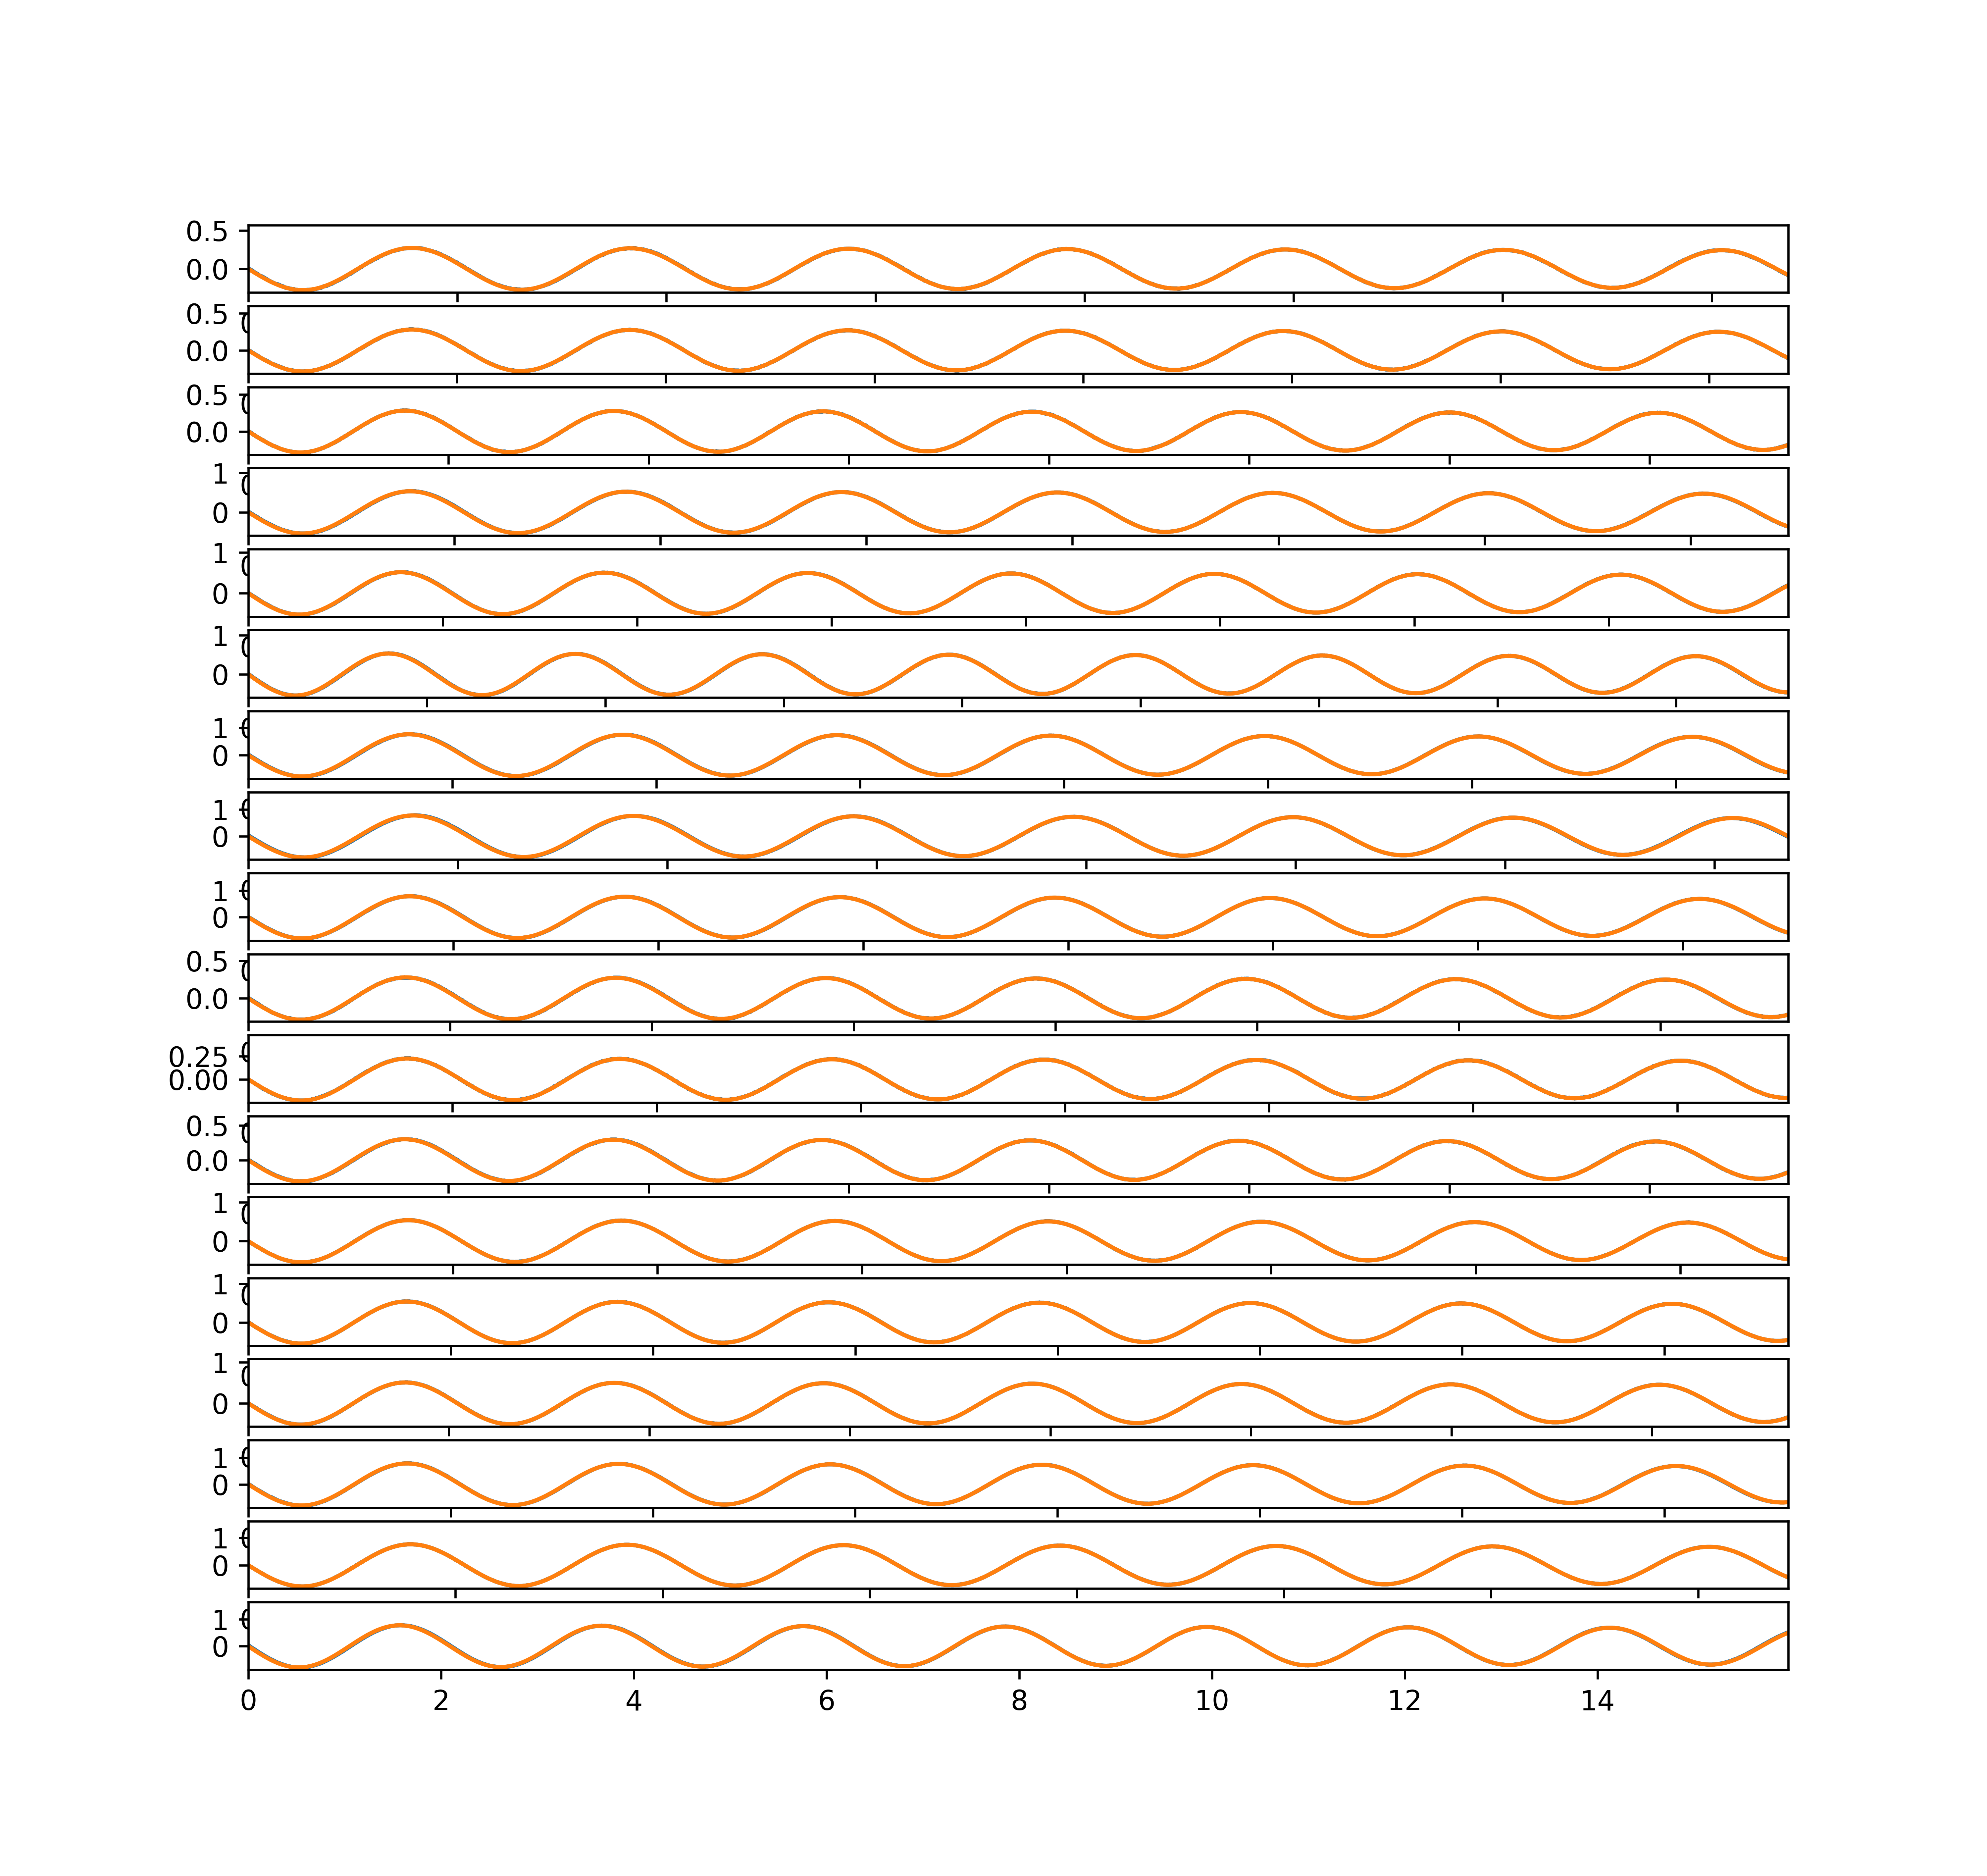
\includegraphics[width = 0.5\textwidth]{figure/damped_oscilation_fitdpi600.png}
    \caption{Fit of skateboard as compound pendulum}
    \label{f_dampedoscillation}
\end{figure}
The inertia results are given in figure \ref{f_inertianopower}
\begin{figure}
    \centering
    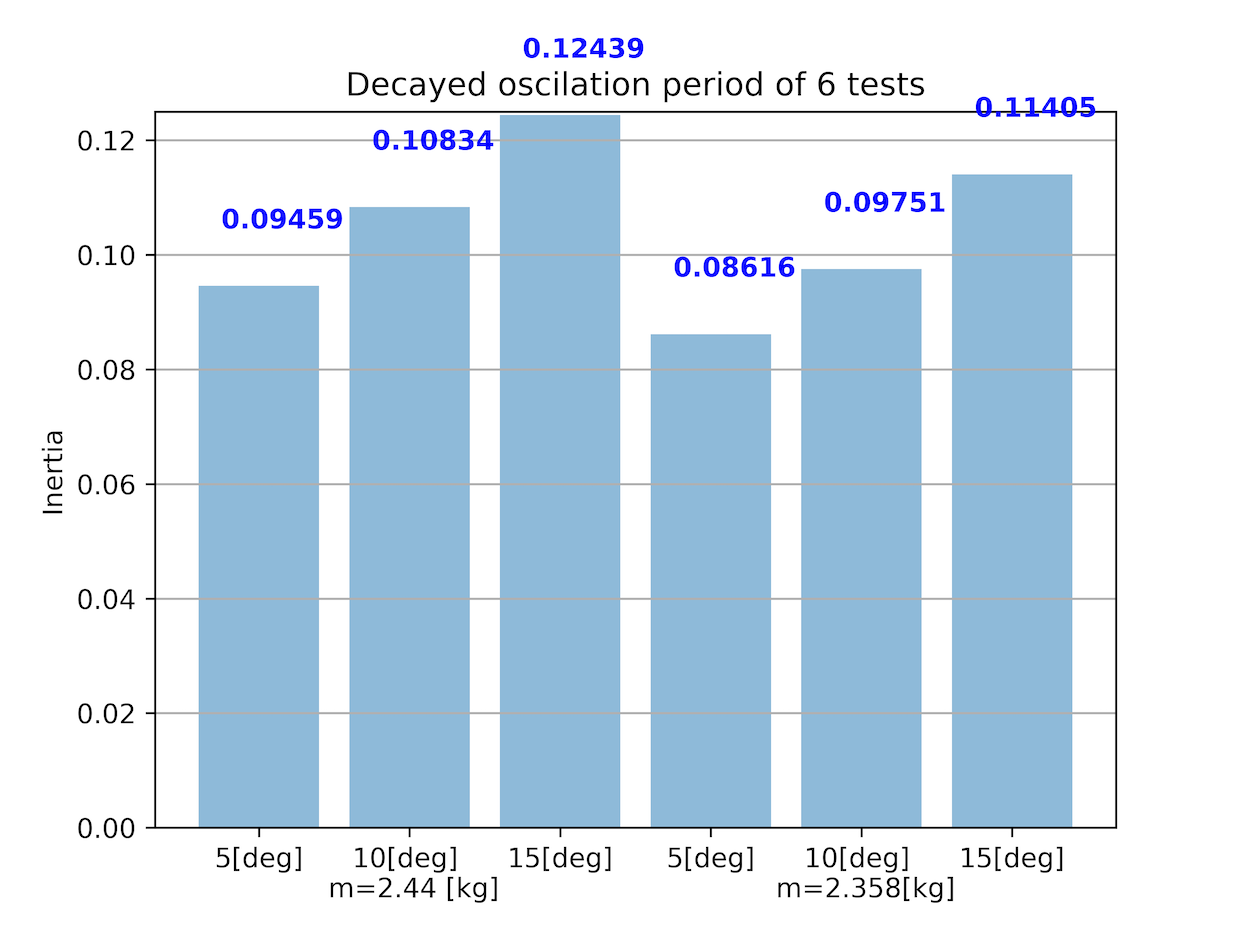
\includegraphics[width = 0.4\textwidth]{figure/Inertia_result_nopowerexpansiondpi600.png}
    \caption{Inertia results}
    \label{f_inertianopower}
\end{figure}
When it was clear that the inertia increased with an increase in starting angle, a power expansion is applied that accounts for small angle errors given by:
\begin{equation}
\begin{array}{r}
\omega_{exact} =  \approx T_0\left(1+\frac{1}{16} \theta^2+\frac{11}{3072} \theta^4+\frac{173}{737280} \theta^6\right. \\
\left.+\frac{22931}{1321205760} \theta^8+\ldots\right) .
\end{array}
\end{equation}
Which is used until the with precision $O^6$ results in the inertia data presented in figure \ref{f_powerexp}

\begin{figure}
    \centering
    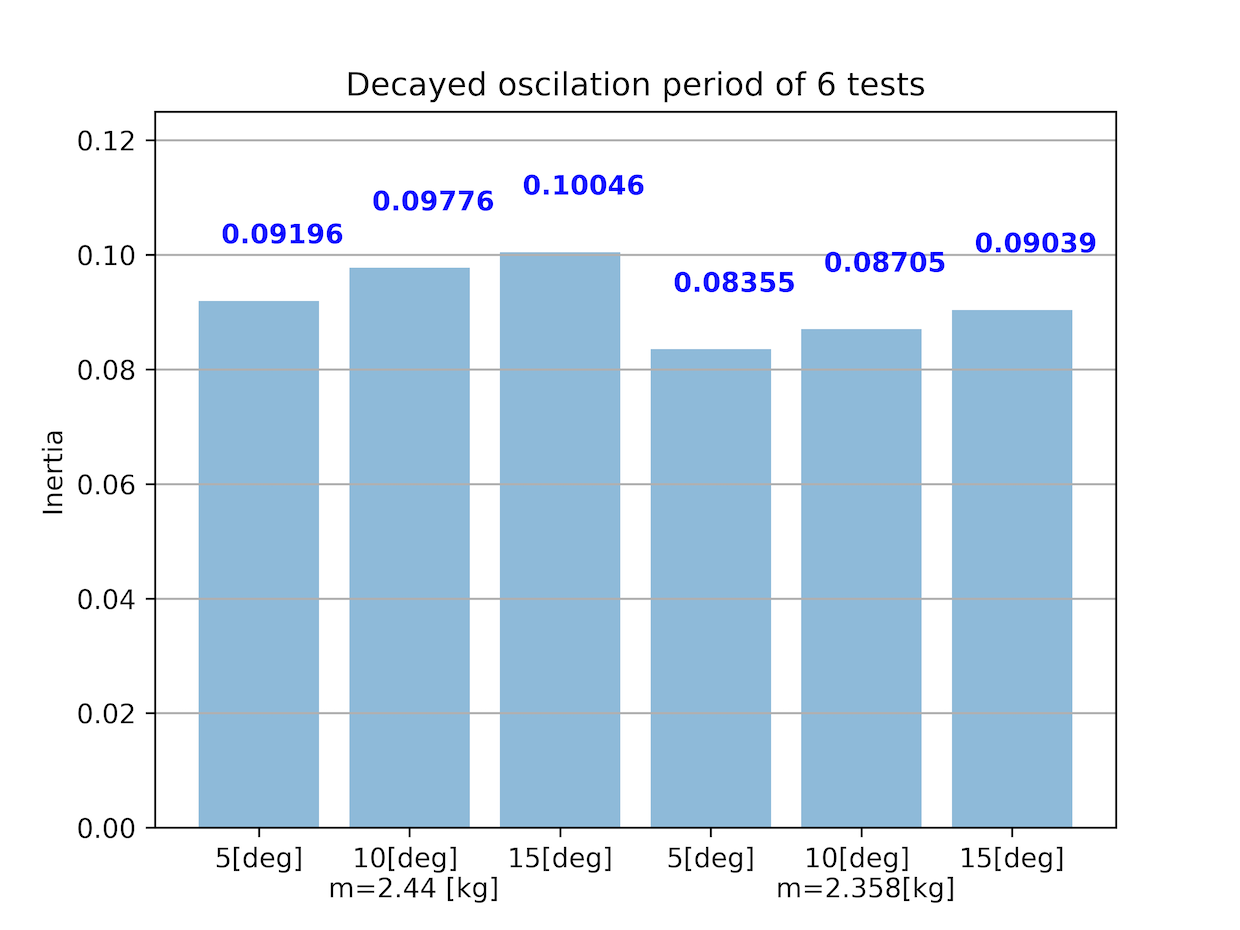
\includegraphics[width = 0.6\textwidth]{figure/Inertia_result_powerexpansiondpi600.png}
    \caption{Inertia result with power expansion}
    \label{f_powerexp}
\end{figure}

The calculated inertia value for skateboard with $m=2.44$ with the parameterized model is: 0.1219 [$kg\ m^2$]. The results show 0.09196 - 0.10046 [$kg\ m^2$]. The skateboards' inertia calculated with the parameterized model  with $m= 2.358$ is 0.1151 [$kg\ m^2$], while the results show 0.08355 - 0.09039 [$kg\ m^2$]. Both skateboards the model slightly overestimates the inertia.   The reduction in real life between the skateboards is 0.909\%, 0.890\%, 0.900\% between the different take off angles and different boards. In the parameterized model reduces inertia by 0.94 \%. This is of similar magnitude but needs more data to make it more exact. As a scaling approximation the parameter model is good enough.

\begin{figure}
    \centering
    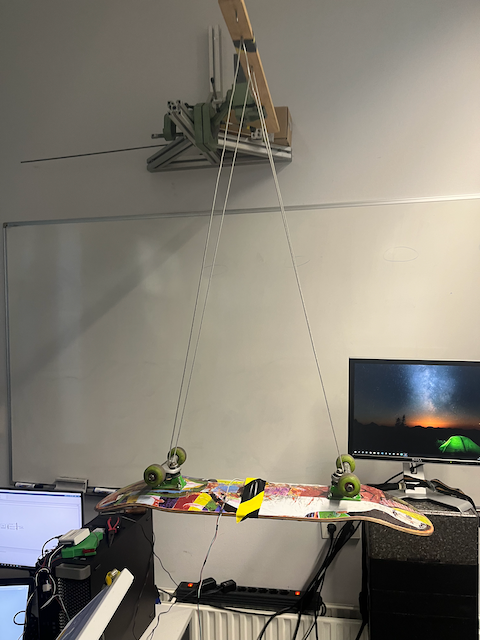
\includegraphics[width = 0.4 \textwidth]{figure/Testsetup.png}
    \caption{Test setup for inertia testing}
    \label{f_testsetup}
\end{figure}

\newpage
.
\newpage
\section*{Mass, centre of mass and inertia model}
\begin{verbatim}
    def Mass_model(width_deck, mass_bearing, mass_truck, height_truck, 
               height_truck0, width_wheel, n_ply, length_flat, length_tail, 
               radius_wheel, rho_pu, rho_maple, rho_steel, m_glue, 
               diameter_axle, d_veneer):

    mass_wheel = rho_pu * sm.pi * width_wheel * \
        ((2*radius_wheel)**2-diameter_axle**2) / 4  # V=pi*h*(D^2-d^2)/4

    mass_axle = sm.pi * (diameter_axle/2)**2 * width_deck * \
        rho_steel  # weight of axle, volume * steel * density

    #    _   _   ___________   _   _
    #  /  | | | |           | | | |  \
    # | 1 | |2| |     3     | |4| | 5 | 6=t1 7=w1 8=t2 9=w2
    #  \ _| |_| |___________| |_| |_ /

    #     1\                  /5
    #      2\_______3________/4
    #        6 \/         \/ 7
    #        8 O 9      10 O 11
    
    # Area of wooden components
    A1 = (1/2) * (1/4) * sm.pi * width_deck**2  # 1/4 pi d^2
    A2 = (length_tail - (width_deck/2)) * width_deck         # l * b
    A3 = length_flat * width_deck           # l * b
    A4 = A2
    A5 = A1
    
    thickness = n_ply*d_veneer
    dV = thickness*rho_maple+(m_glue/2*(n_ply-2))

    m1 = A1 * dV
    m2 = A2 * dV
    m3 = A3 * dV
    m4 = m2
    m5 = m1
    m6 = (mass_truck - mass_axle) * height_truck/height_truck0
    m7 = m6
    m8 = mass_axle
    m9 = 2*mass_wheel
    m10 = m8
    m11 = m9

    mass = [m1, m2, m3, m4, m5, m6, m7, m8, m9, m10, m11]
    return mass

def COM(mass, com_points, reference_point):
    # Function gets vector position from reference_point
    # Then assigns COM location to point COM
    # Returns position vector of COM points relative to COM
    r_m = []
    for i, x in enumerate(com_points):
        r_m.append(x.pos_from(reference_point)*mass[i])
    COM_skateboard = me.Point('COM_skateboard')
    COM_skateboard.set_pos(reference_point, (sum(r_m)/sum(mass)))
    return COM_skateboard
\end{verbatim}
\newpage
\begin{verbatim}
    
def Inertia_model(mass, com_points, com, majordim, shape):
    # Major dim:
    #   - (semi)cylinder;  diameter
    #   - cuboid: [l,h]
    #   - Triangle: [Base, Height]

    I_com = []
    I_steiner = []

    for i in range(len(mass)):
        if shape[i] == 'semicircle':
            I_com.append(((1/4)-(16/(9*sm.pi**2)))*mass[i]*(majordim[i]/2)**2)

        if shape[i] == 'cuboid':
            I_com.append((mass[i]/12) * (majordim[i]
                         [0]**2 + majordim[i][1]**2))

        if shape[i] == 'triangle':
            s = sm.sqrt((majordim[i][0]/2)**2+majordim[i][1]**2)
            beta = 2*sm.asin((majordim[i][0]/2)/s)
            I_com.append((mass[i]/2)*s**2*(1-(2/3)*sm.sin(beta)))

        if shape[i] == 'cylinder':
            I_com.append((1/2)*mass[i]*(majordim[i]/2)**2)
        #Trigsimp was sometimes necesarry due to a theta still being in there
        I_steiner.append(sm.trigsimp(mass[i]*d2s(sm.sqrt(com_points[i].\
        pos_from(com).dot(A.x)**2+com_points[i].pos_from(com).dot(A.y)**2)**2)))
    I_tot = sum(I_com)+sum(I_steiner)
    return I_tot, I_com, I_steiner
\end{verbatim}

%\section*{Appendix B: Figures and tables}
\begin{table*}[h]
\begin{center}
\caption[Numerical bounds of state variables]{\centering Numerical bounds to state variables in the order of initial - absolute - final bounds. Final bound of $p^{(n)}$ equals initial bound of $p^{(n+1)}$. $v_{bound} = [-50,50]$} 
\begin{tabular}{r l l l l l l l l}\label{t_constraints}
& & \\ % put some space after the caption
\hline
ID         & Variable   & $p_0^{(1)}$ & $p^{(1)}_{bounds}$& $p_F^{(1)} = p_0^{2}$ & $p^{(2)}_{bounds}$ &$p_F^{(2)} = p_0^{(3)}$& $p^{(3)}_{bounds}$ &$p_F^{(3)}$  \\
\hline
\rownumber & $x_w$      & [-1, 0]     & [-2,1]            & [-2,1]               & -                  & -                   &  -                  & -\\
\rownumber & $x_s$      & -           & -                 &[-1,1]                & [-1,1]             & [-1, 1]             &  [-1,1]             & [-1,1]   \\
\rownumber & $y_s$      & -           & -                 &[0, 2]                & [0,5]              & [0, 5]              &  [0,5]              & [0,1] \\
\rownumber & $\theta_s$ & 0           & [0,$\pi$/2]       &[0, $\pi$/2 ]         & [-$\pi$/2 ,$\pi$/4]& 0                   & [$-\pi$/2, $\pi$/4] & [0, $\pi$/6]\\
\rownumber & $s_1$      & [0,1]       & [0,1]             &[0,1]                 & [0,1]              & [0,1]               & [0,1]              & [0,1]\\
\rownumber & $s_2 $     & [0,1]       & [0,1]             &[0,1]                 & [0,1]              & [0,1]               & [0,1]              & [0,1]\\
\rownumber & $x_h $     & 0           & [-1,1]            &[-1,1]                & [-1,1]             & [-1,1]              & [-1,1]             & [-1,1]\\
\rownumber & $y_h $     & [0,2]       & [0,5]             &[0,5]                 & [0,5]              & [0,5]               & [0,5]              & [0,5]\\
\rownumber & $\dot x_w$ & -           & $v_{bound}$       & $v_{bound}$          & -                  & -                   &  -                 &\\
\rownumber & $\dot x_s$ & 0           & $v_{bound}$       & $v_{bound}$          &$v_{bound}$         &$v_{bound}$          & $v_{bound}$        & $v_{bound}$  \\
\rownumber & $\dot y_s$ & 0           & $v_{bound}$       & $v_{bound}$          &$v_{bound}$         & 0                   &$v_{bound}$        & $v_{bound}$\\
\rownumber & $\dot \theta_s$ & 0      & $v_{bound}$       & $v_{bound}$          &$v_{bound}$         & $v_{bound}$         &$v_{bound}$        & $v_{bound}$ \\
\rownumber & $\dot s_1$ & 0           & $v_{bound}$       & $v_{bound}$          &$v_{bound}$         & $v_{bound}$         &$v_{bound}$        & $v_{bound}$ \\
\rownumber & $\dot s_2 $& 0           & $v_{bound}$       & $v_{bound}$          &$v_{bound}$         & $v_{bound}$         &$v_{bound}$        & $v_{bound}$ \\
\rownumber & $\dot x_h $& 0           & $v_{bound}$       & $v_{bound}$          &$v_{bound}$         & $v_{bound}$         &$v_{bound}$        & $v_{bound}$ \\
\rownumber & $\dot y_h $& 0           & $v_{bound}$       & $v_{bound}$          &$v_{bound}$         & $v_{bound}$         &$v_{bound}$        & $v_{bound}$ \\

\hline
\end{tabular}
\end{center}
\end{table*}
\section*{Results of optimal board shapes}
Detailed trajectories, states and control of all optimizations shown in figures \ref{f_nopar}, \ref{f_singlepar}, and \ref{f_multipar}
\begin{figure*}[b]
    \subfloat[Long board]{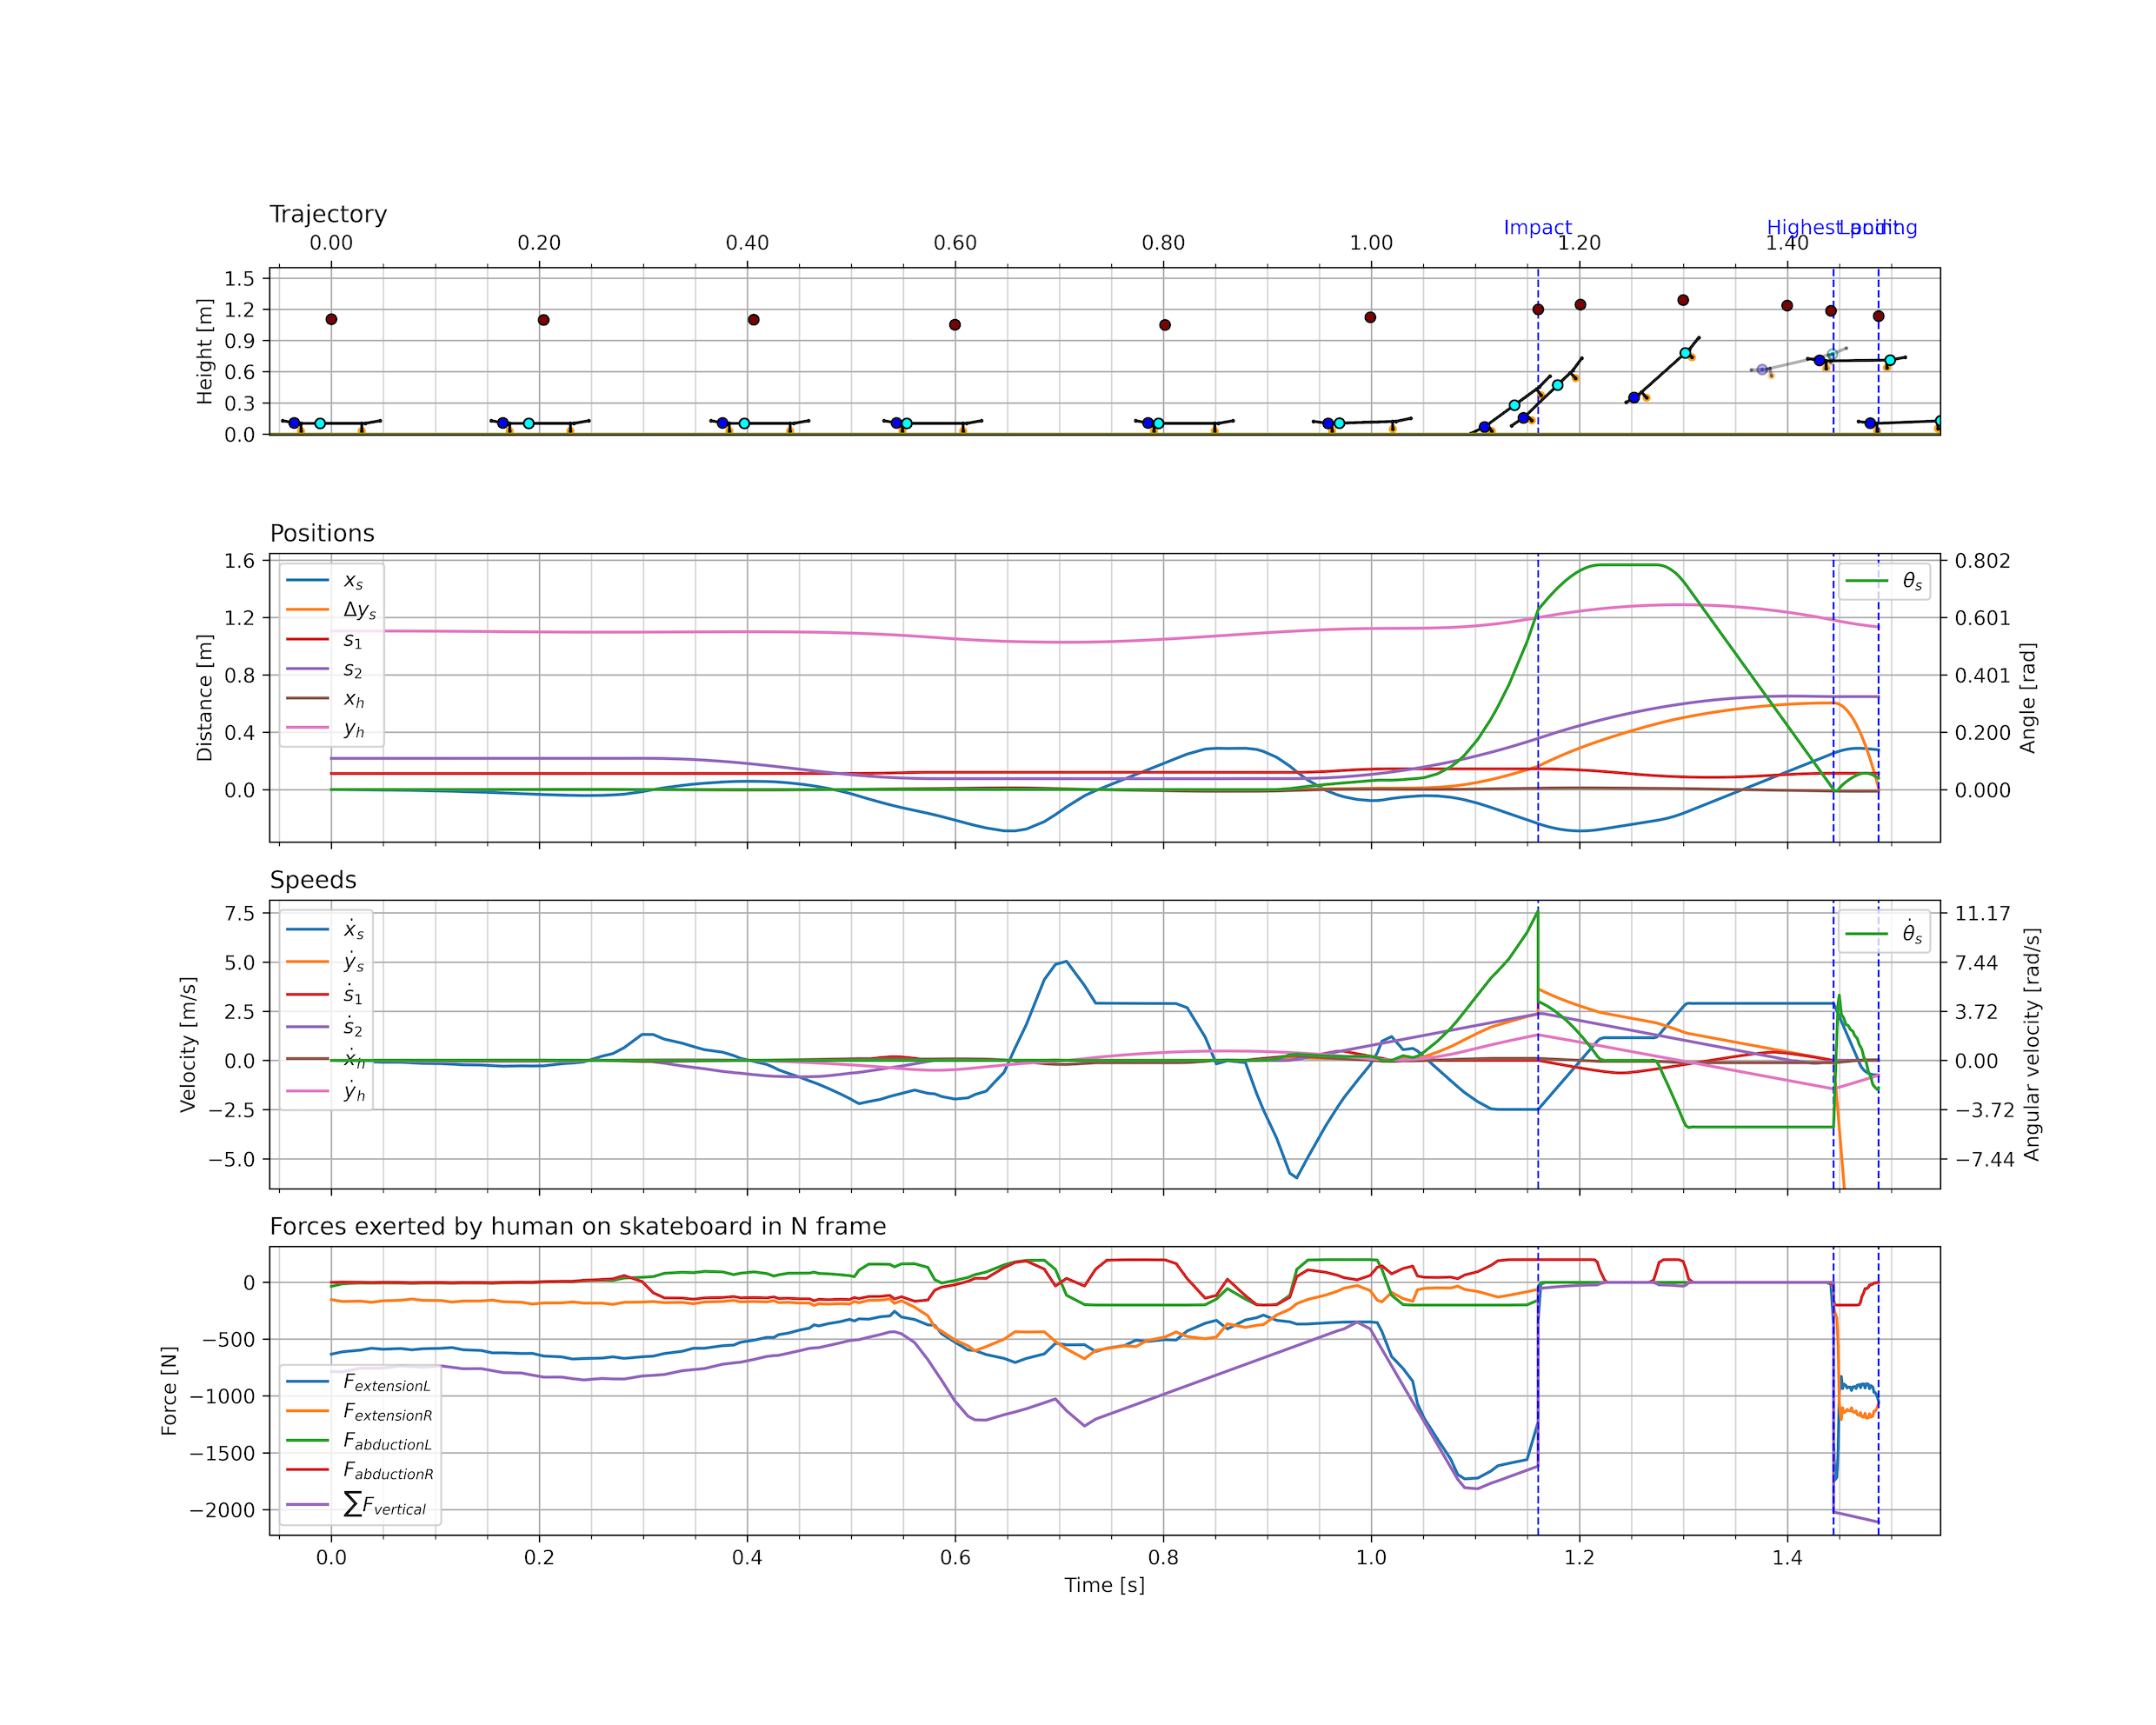
\includegraphics[trim={0cm 0cm 0cm 0cm},clip,width=0.8\textwidth]{figure/Results/data_longboard_init_longer_tail_optdpi600.png}}
    \newline
    \subfloat[All parameters no trucks]{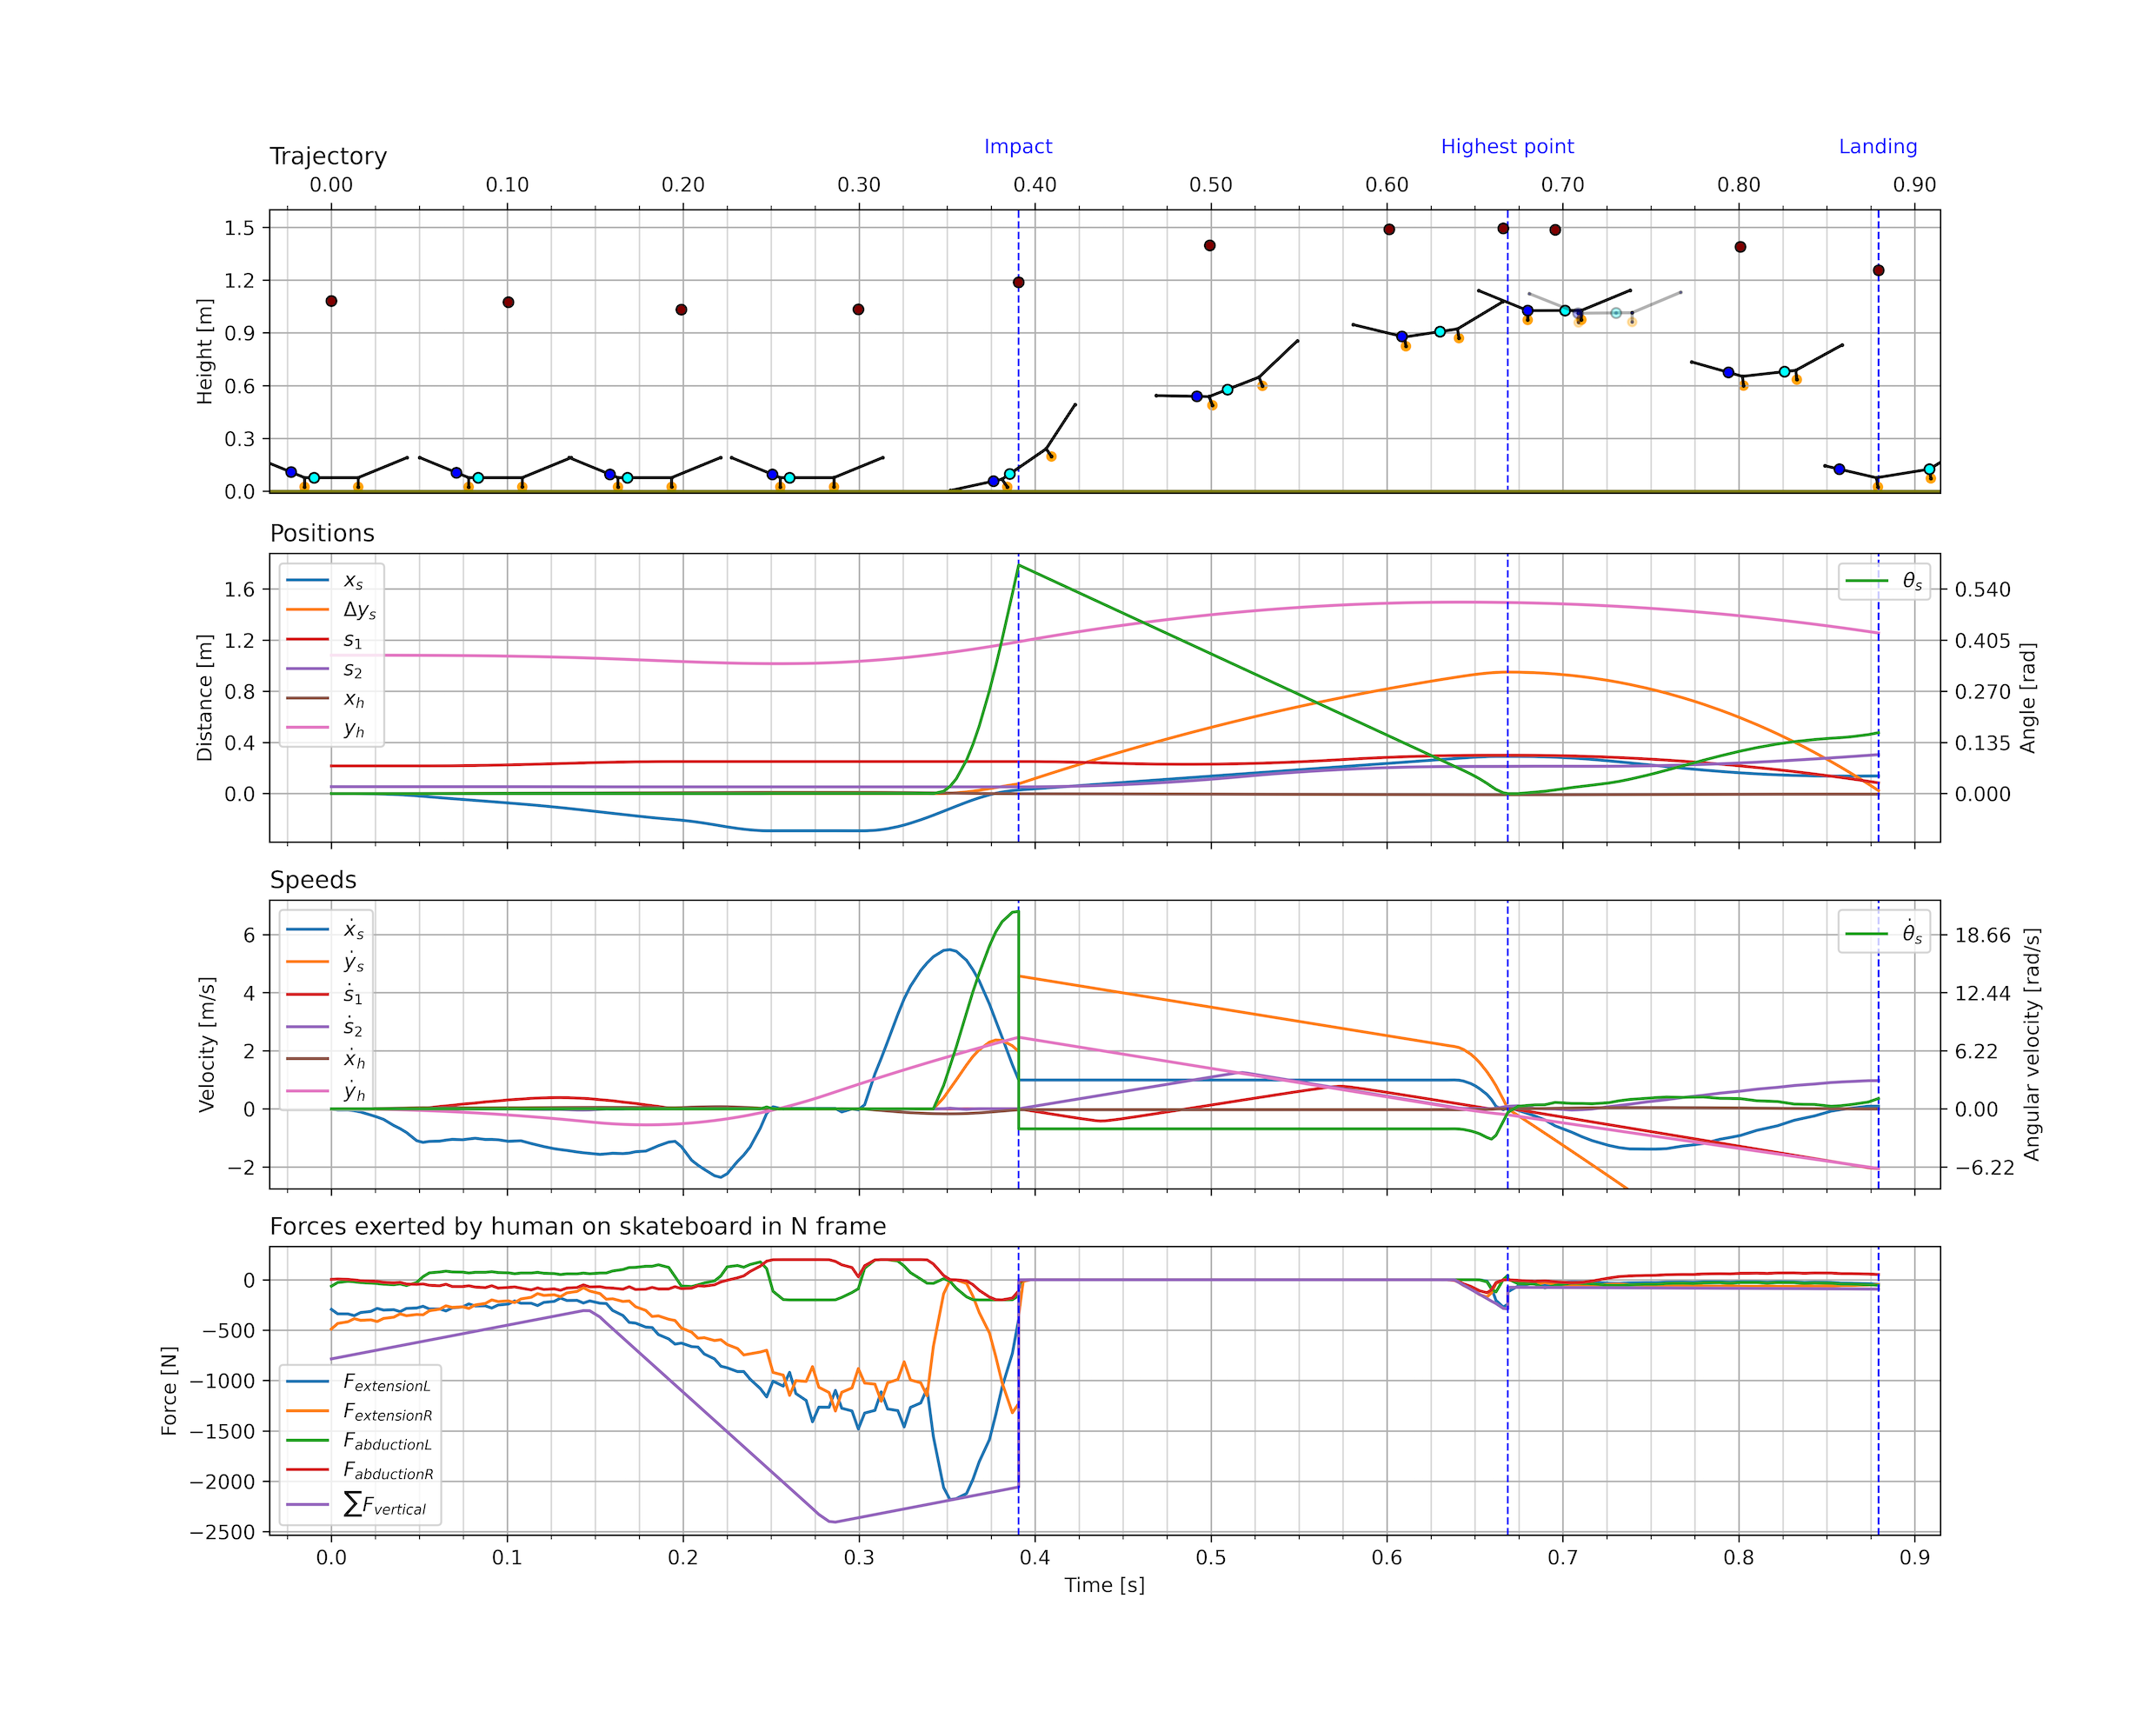
\includegraphics[trim={0cm 0cm 0cm 0cm},clip,width=0.8\textwidth]{figure/Results/data_notrrwdpi600.png}}
    \label{f_longboard}
    \caption{Longboard and `all except trucks' optimization results}
\end{figure*}

\begin{figure*}[b]    
    \subfloat[Plastic]{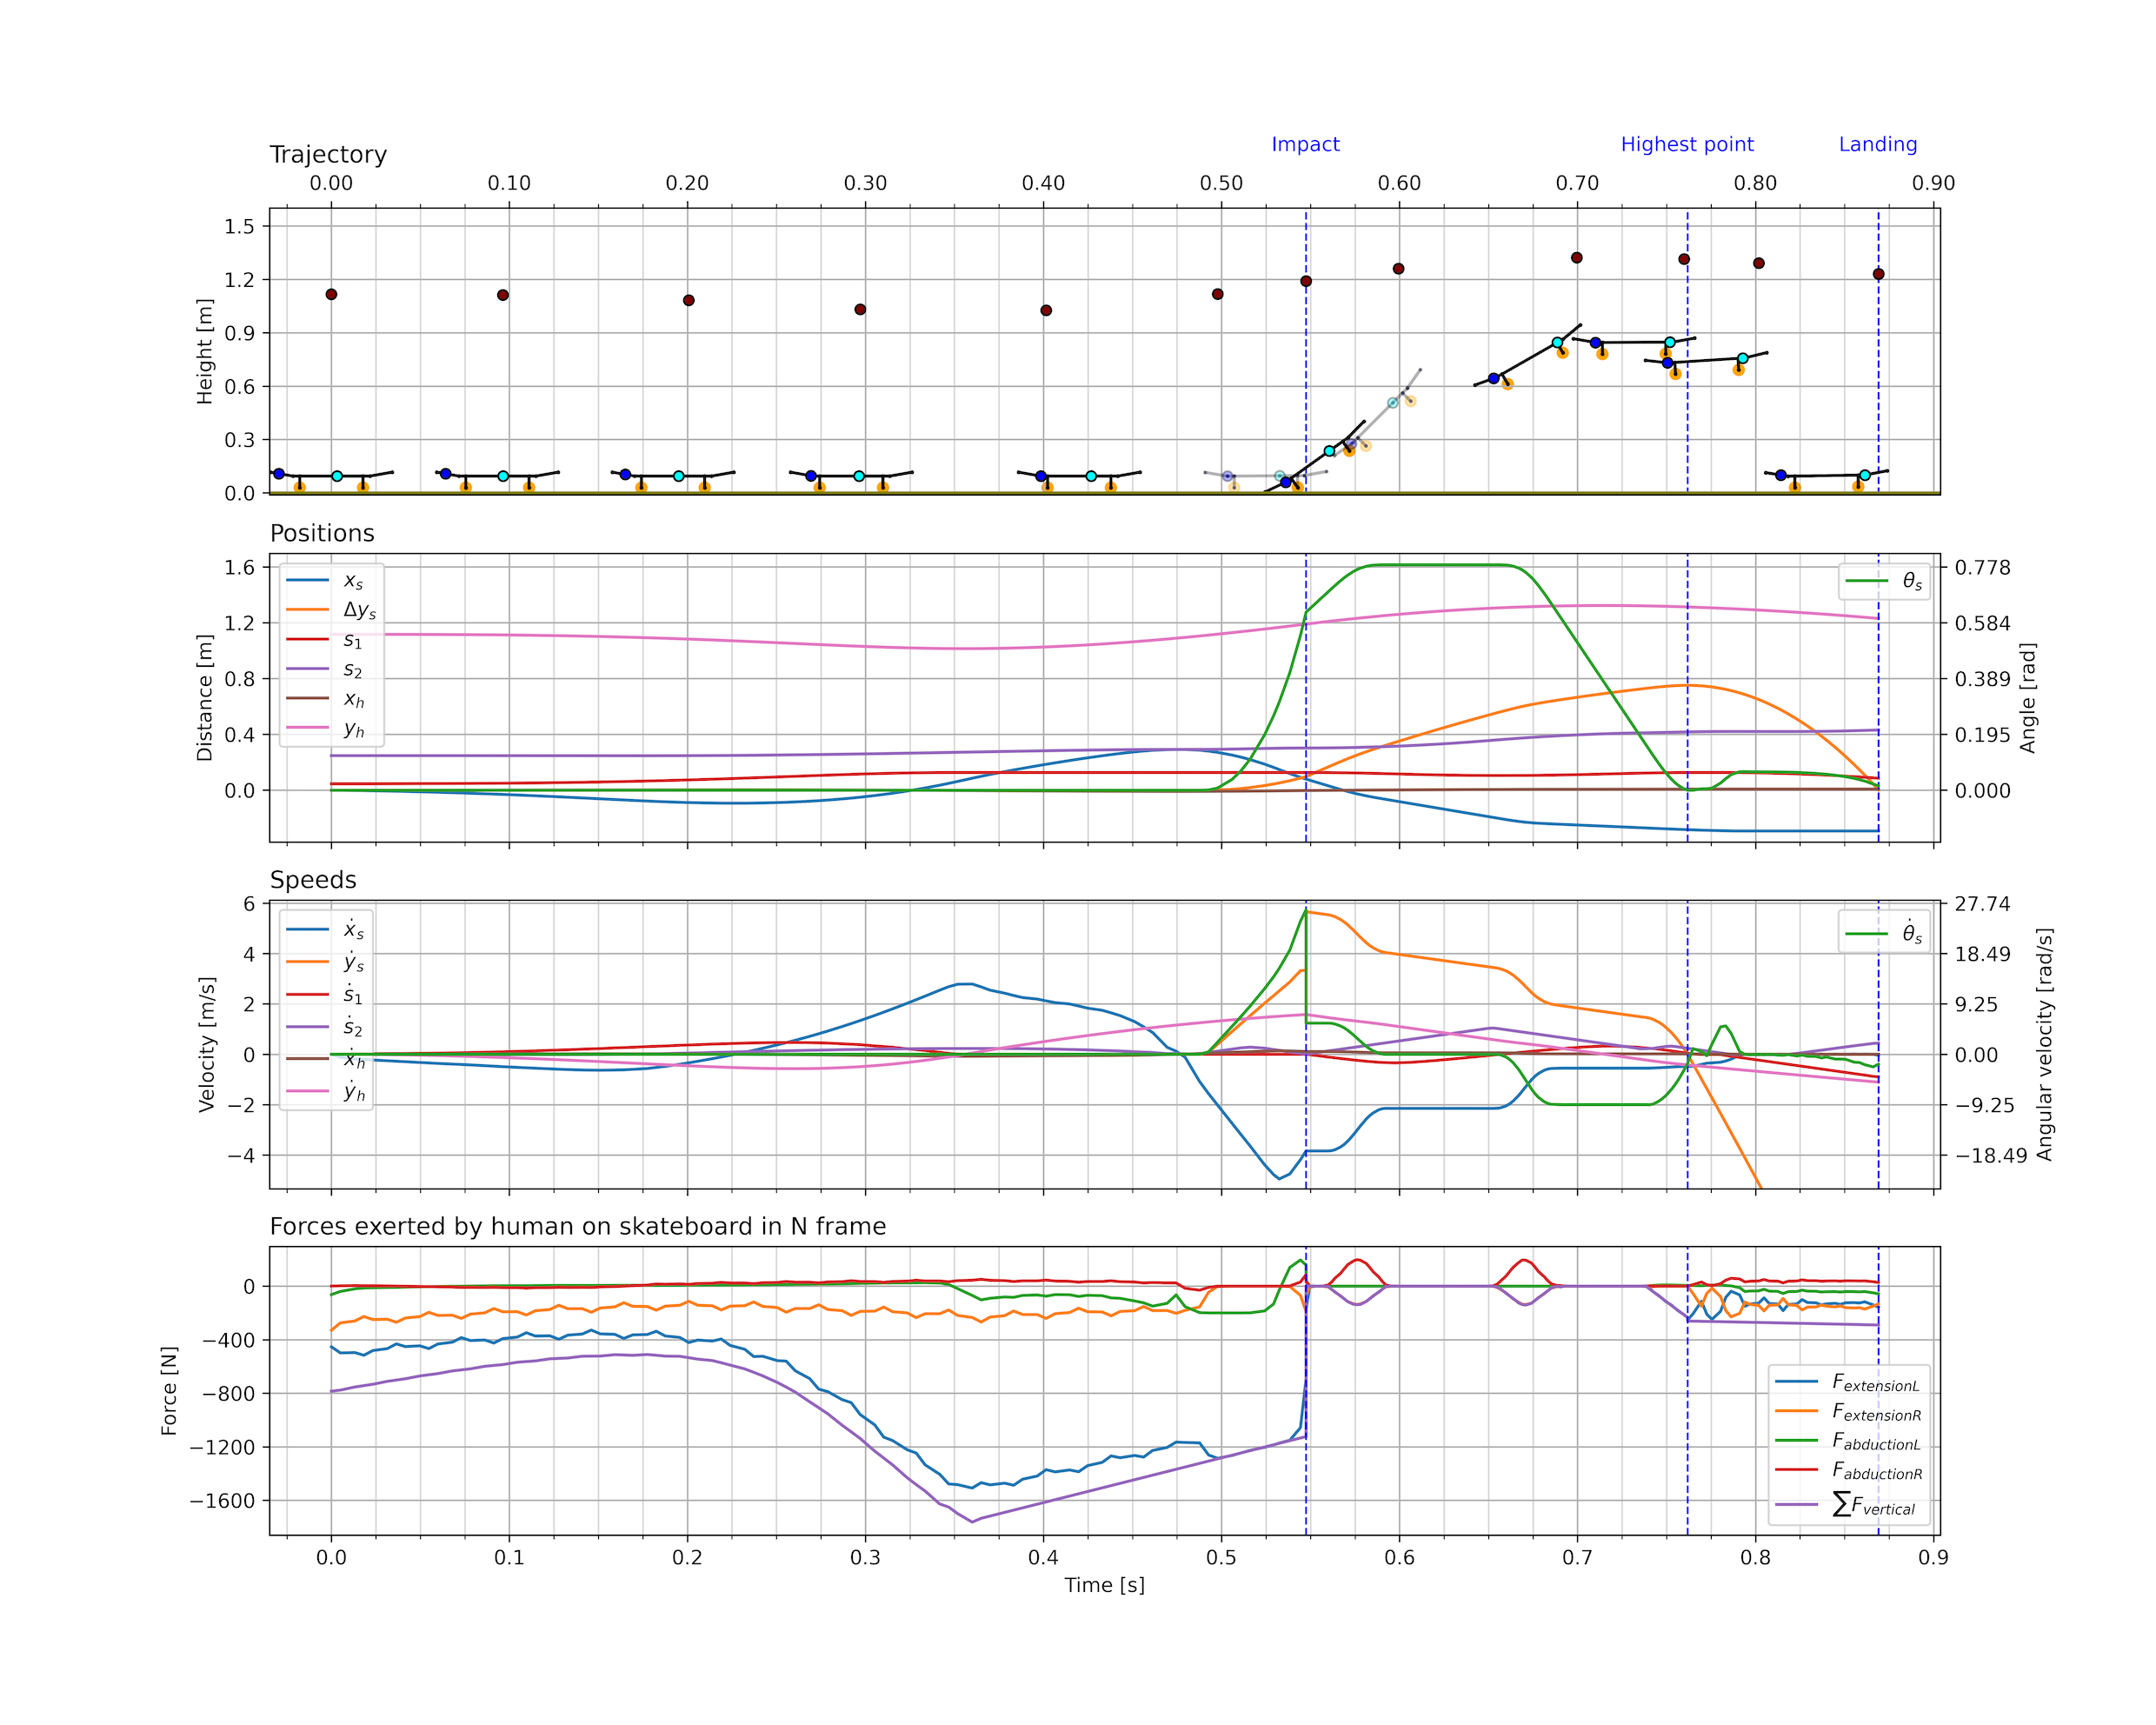
\includegraphics[trim={0cm 0cm 0cm 0cm},clip,width=0.8\textwidth]{figure/Results/data_penny_02dpi600.png}}
    \newline
    \subfloat[Griptape]{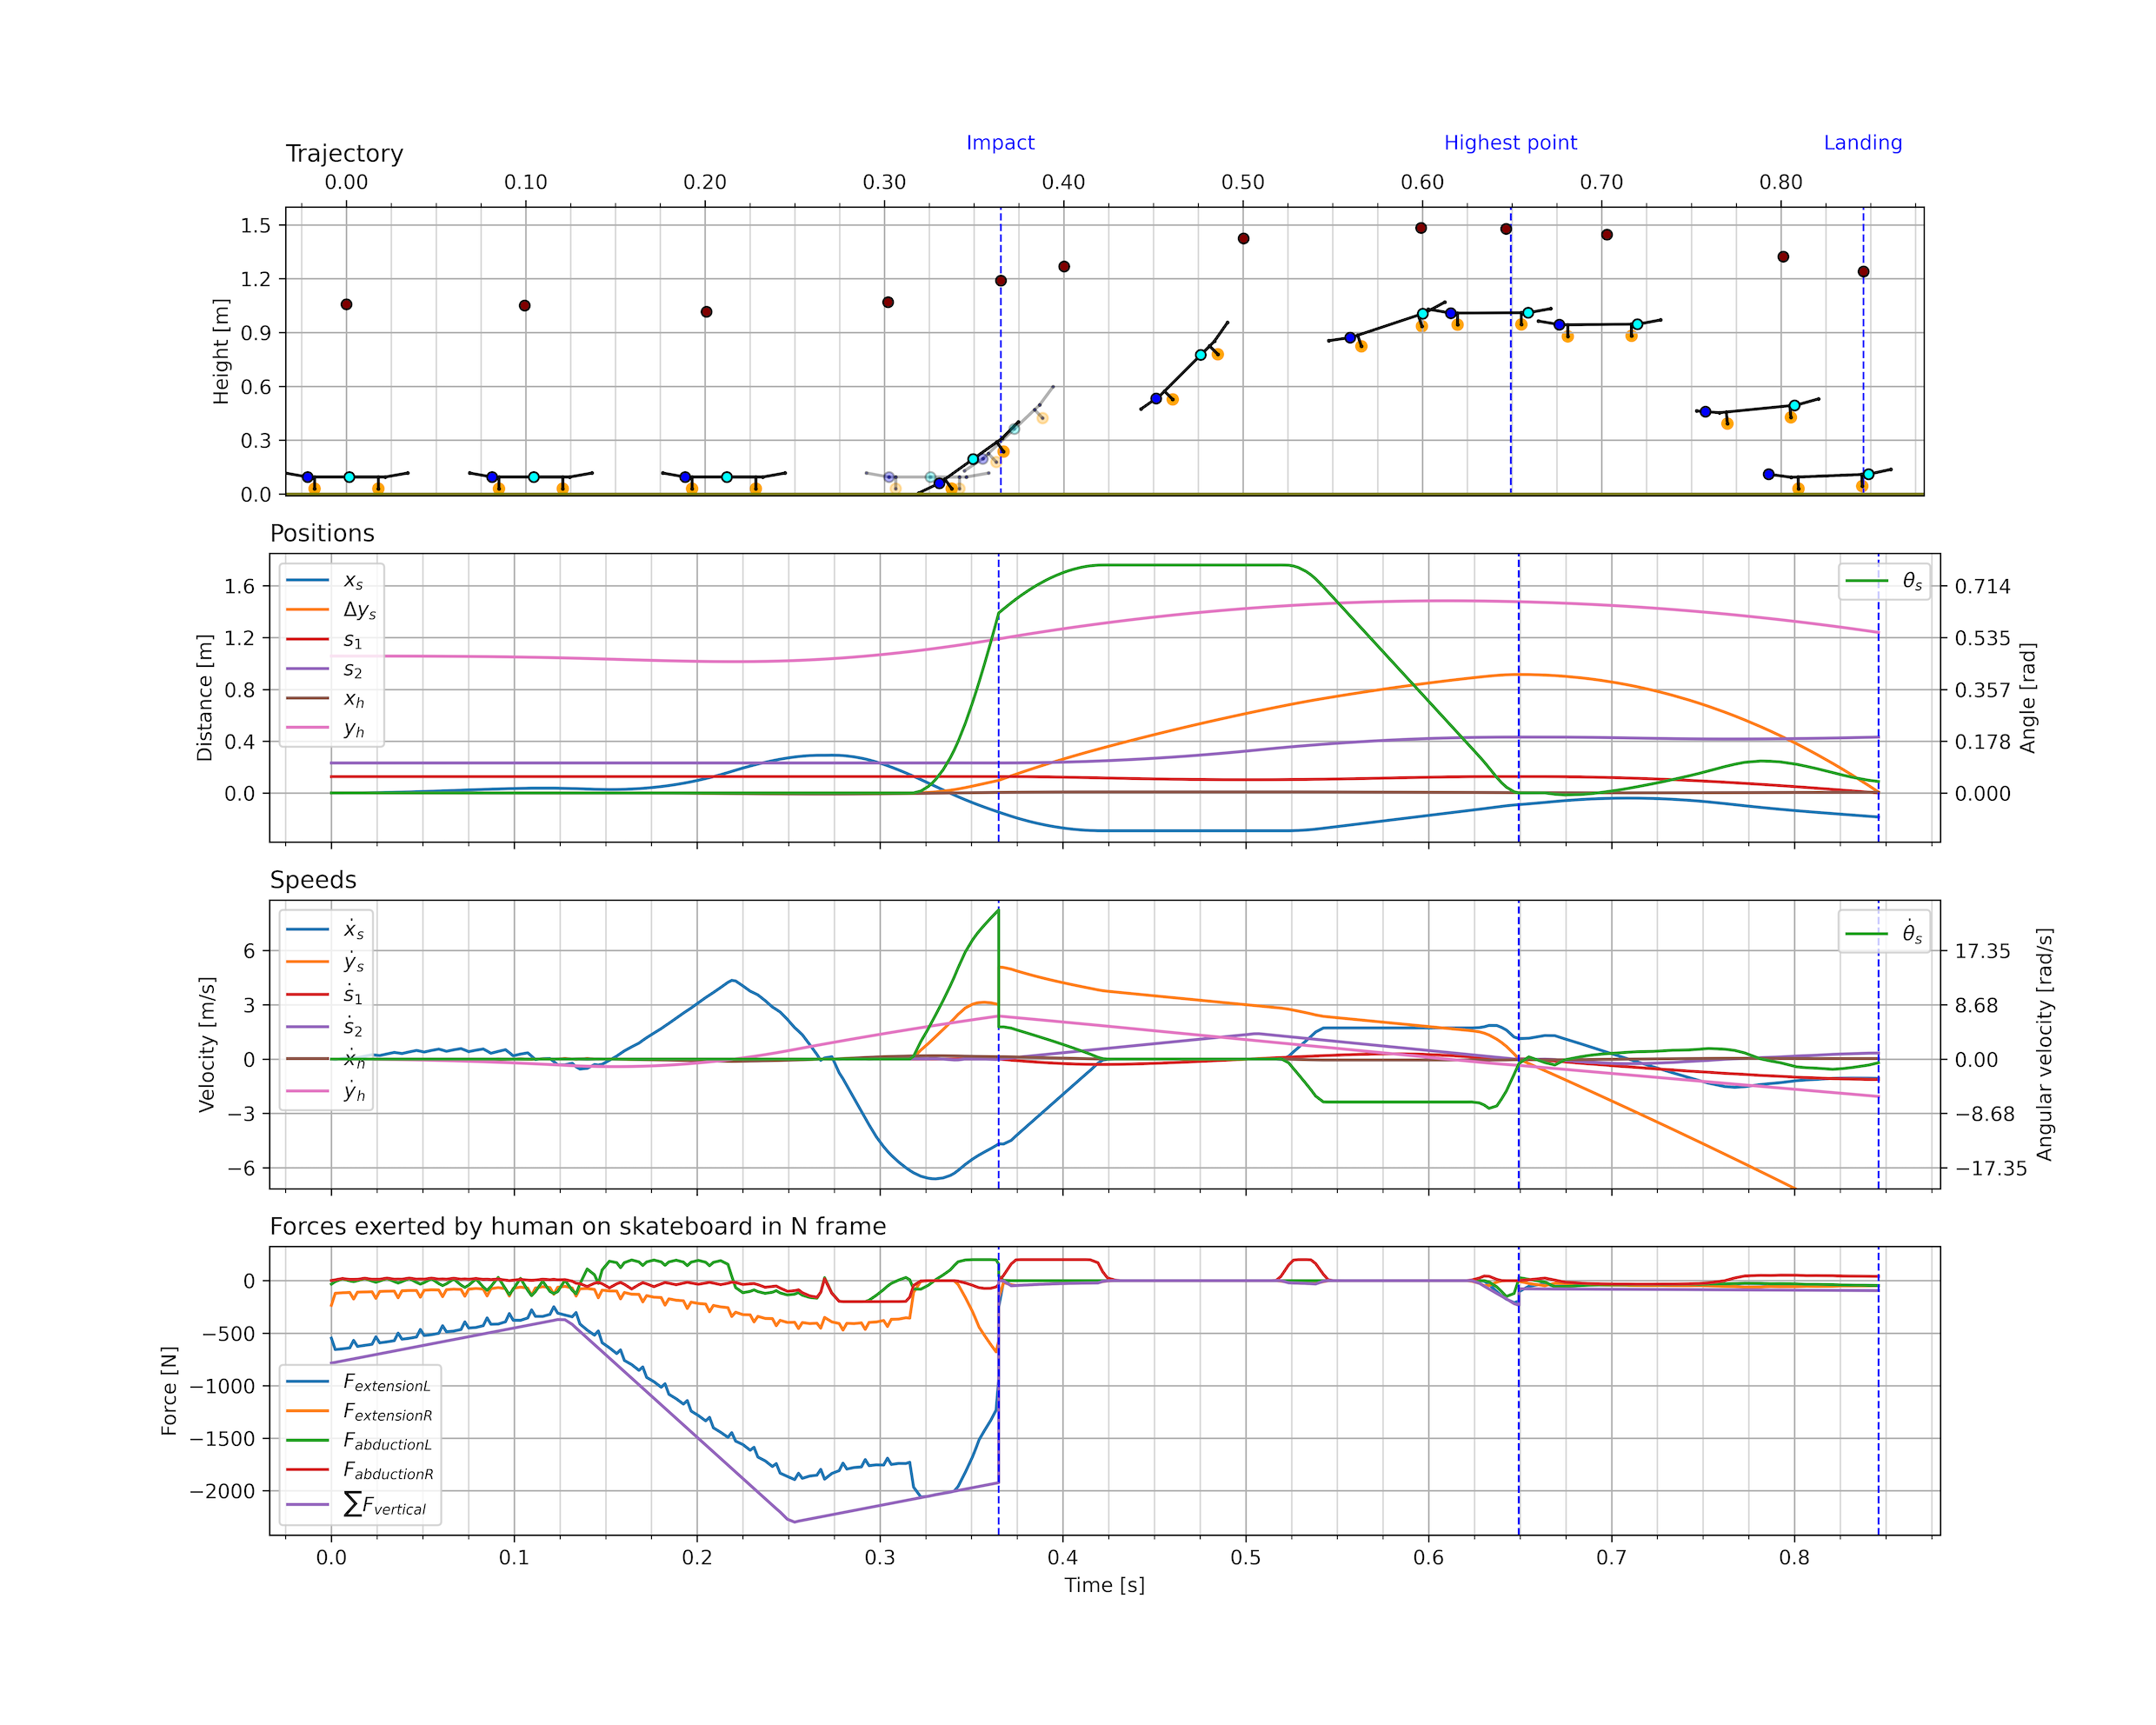
\includegraphics[trim={0cm 0cm 0cm 0cm},clip,width=0.8\textwidth]{figure/Results/data_penny_08dpi600.png}}
    \caption{Penny boards optimization results}    
\end{figure*}

\begin{figure*}[b]    
    \subfloat[Wheel radius]{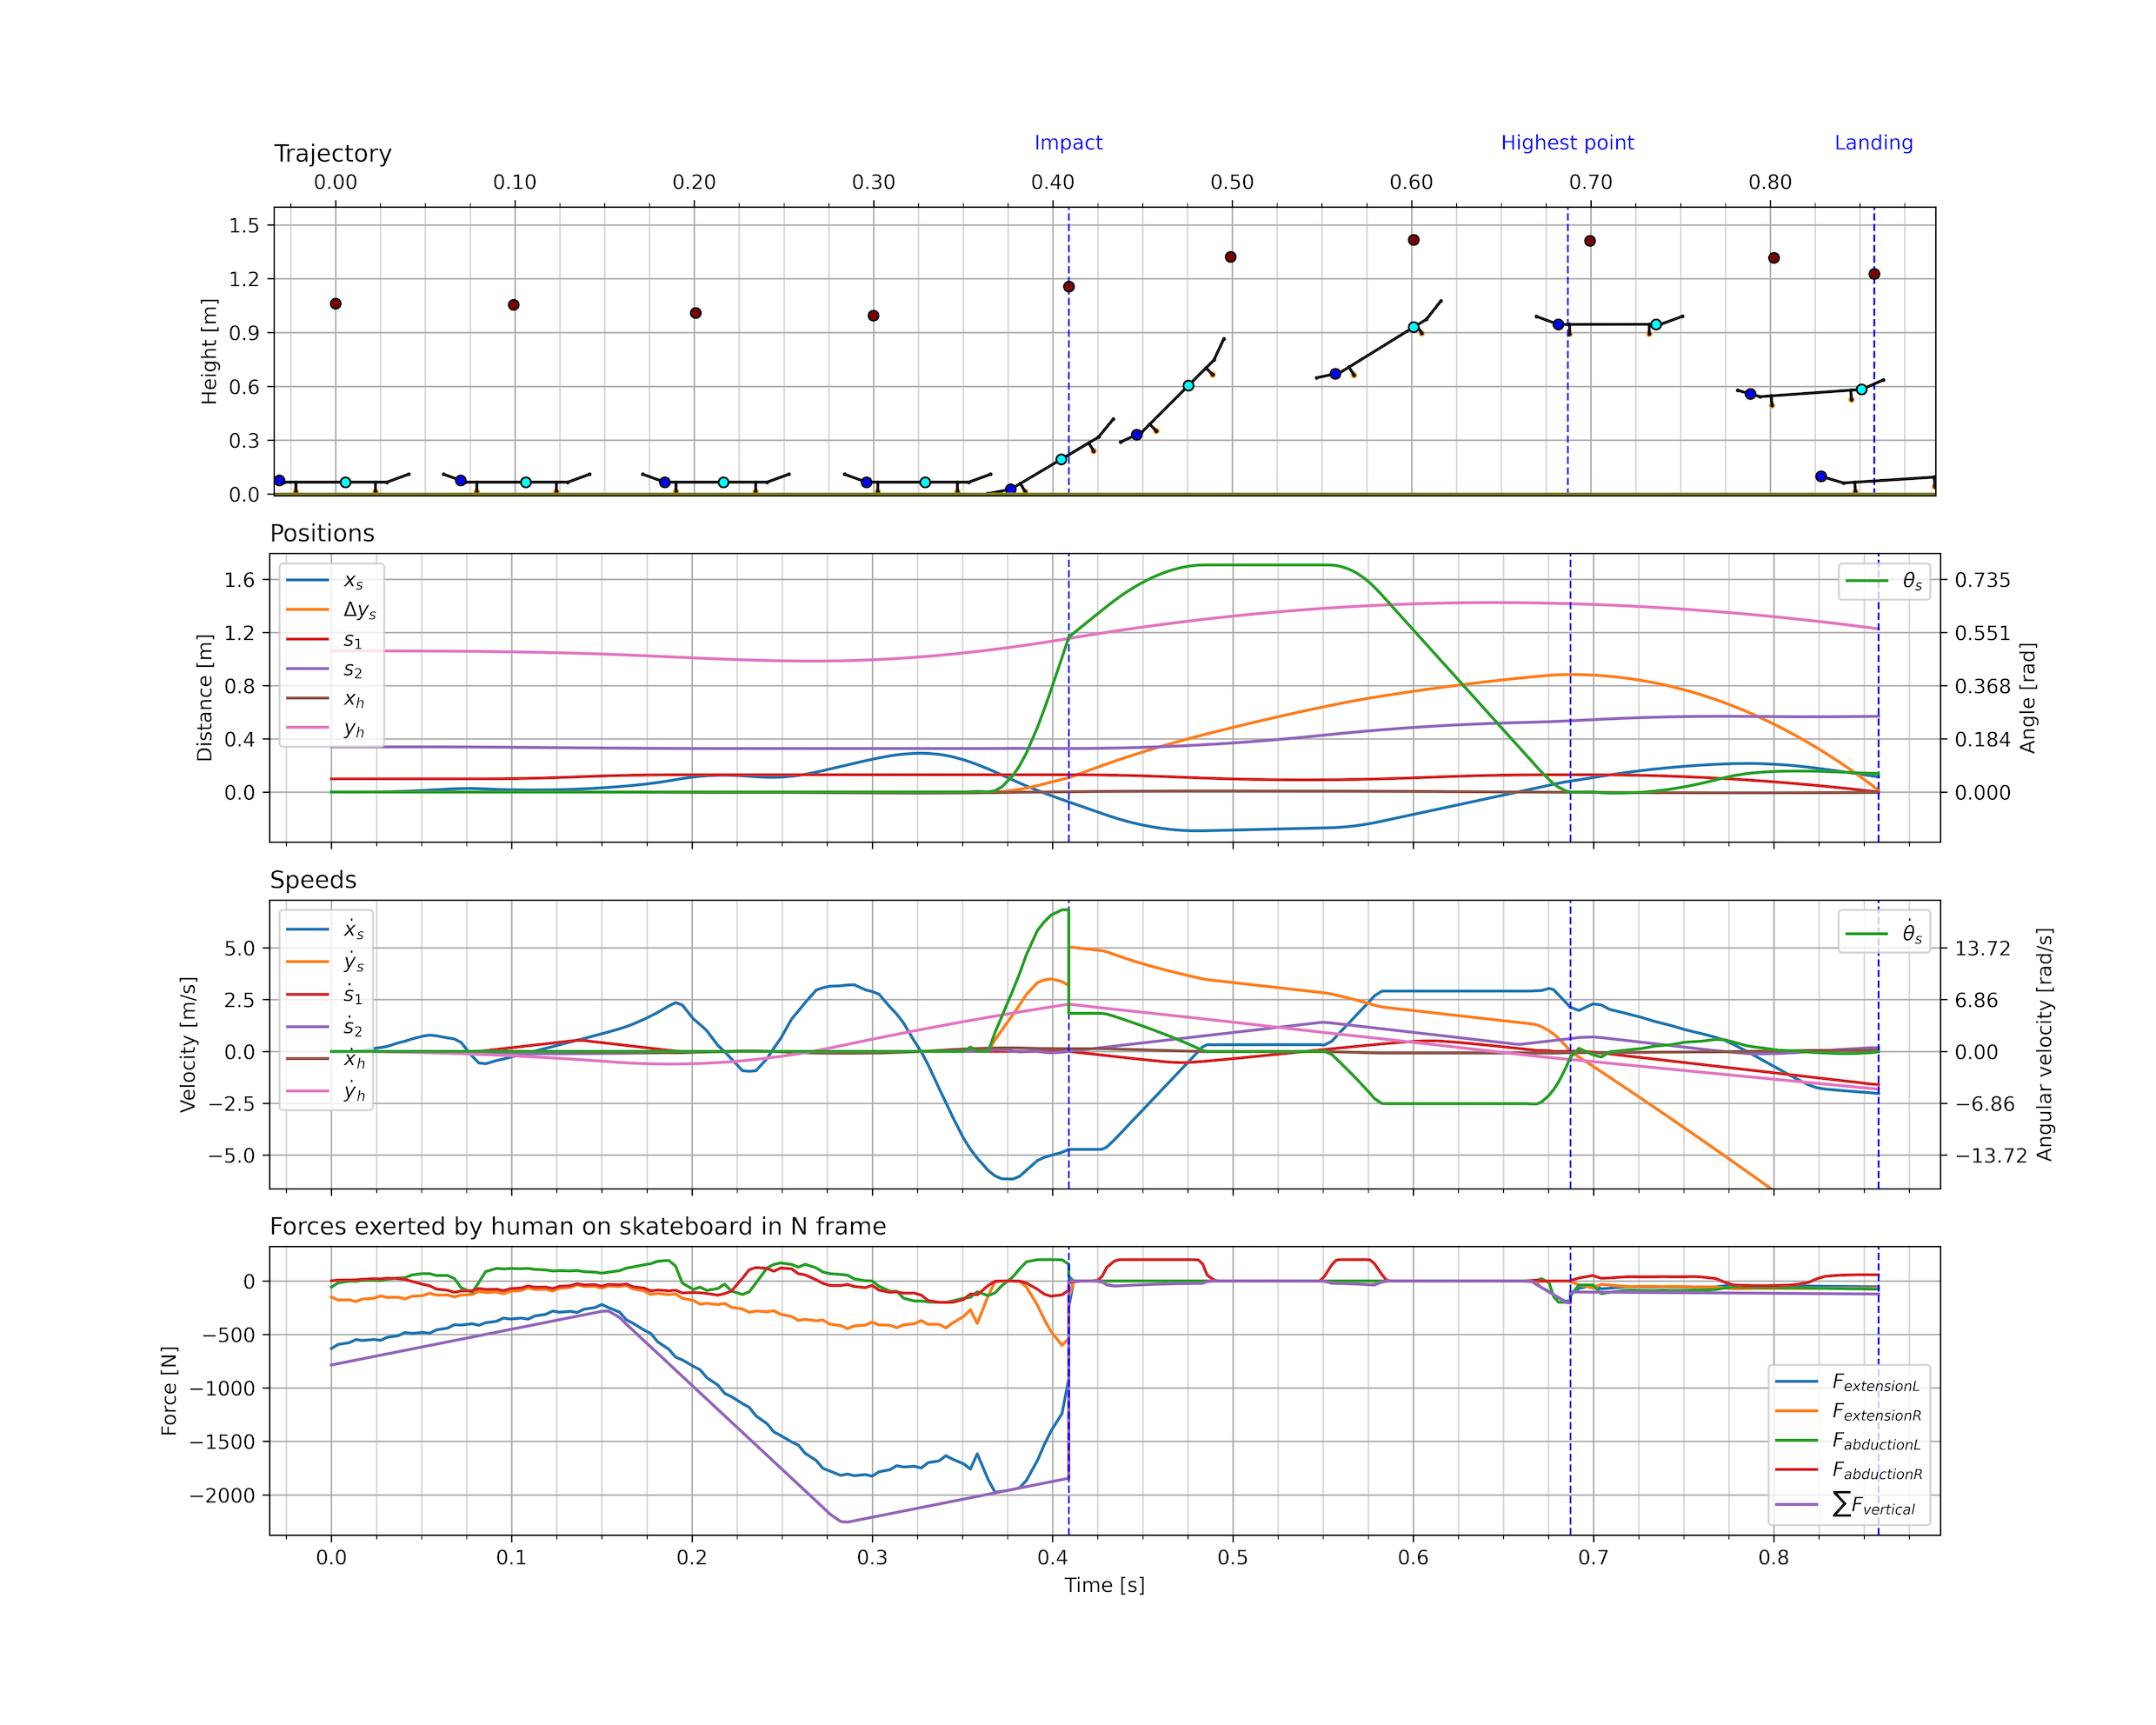
\includegraphics[trim={0cm 0cm 0cm 0cm},clip,width=0.8\textwidth]{figure/Results/data_r_wdpi600.png}}
    \newline
    \subfloat[Truck height]{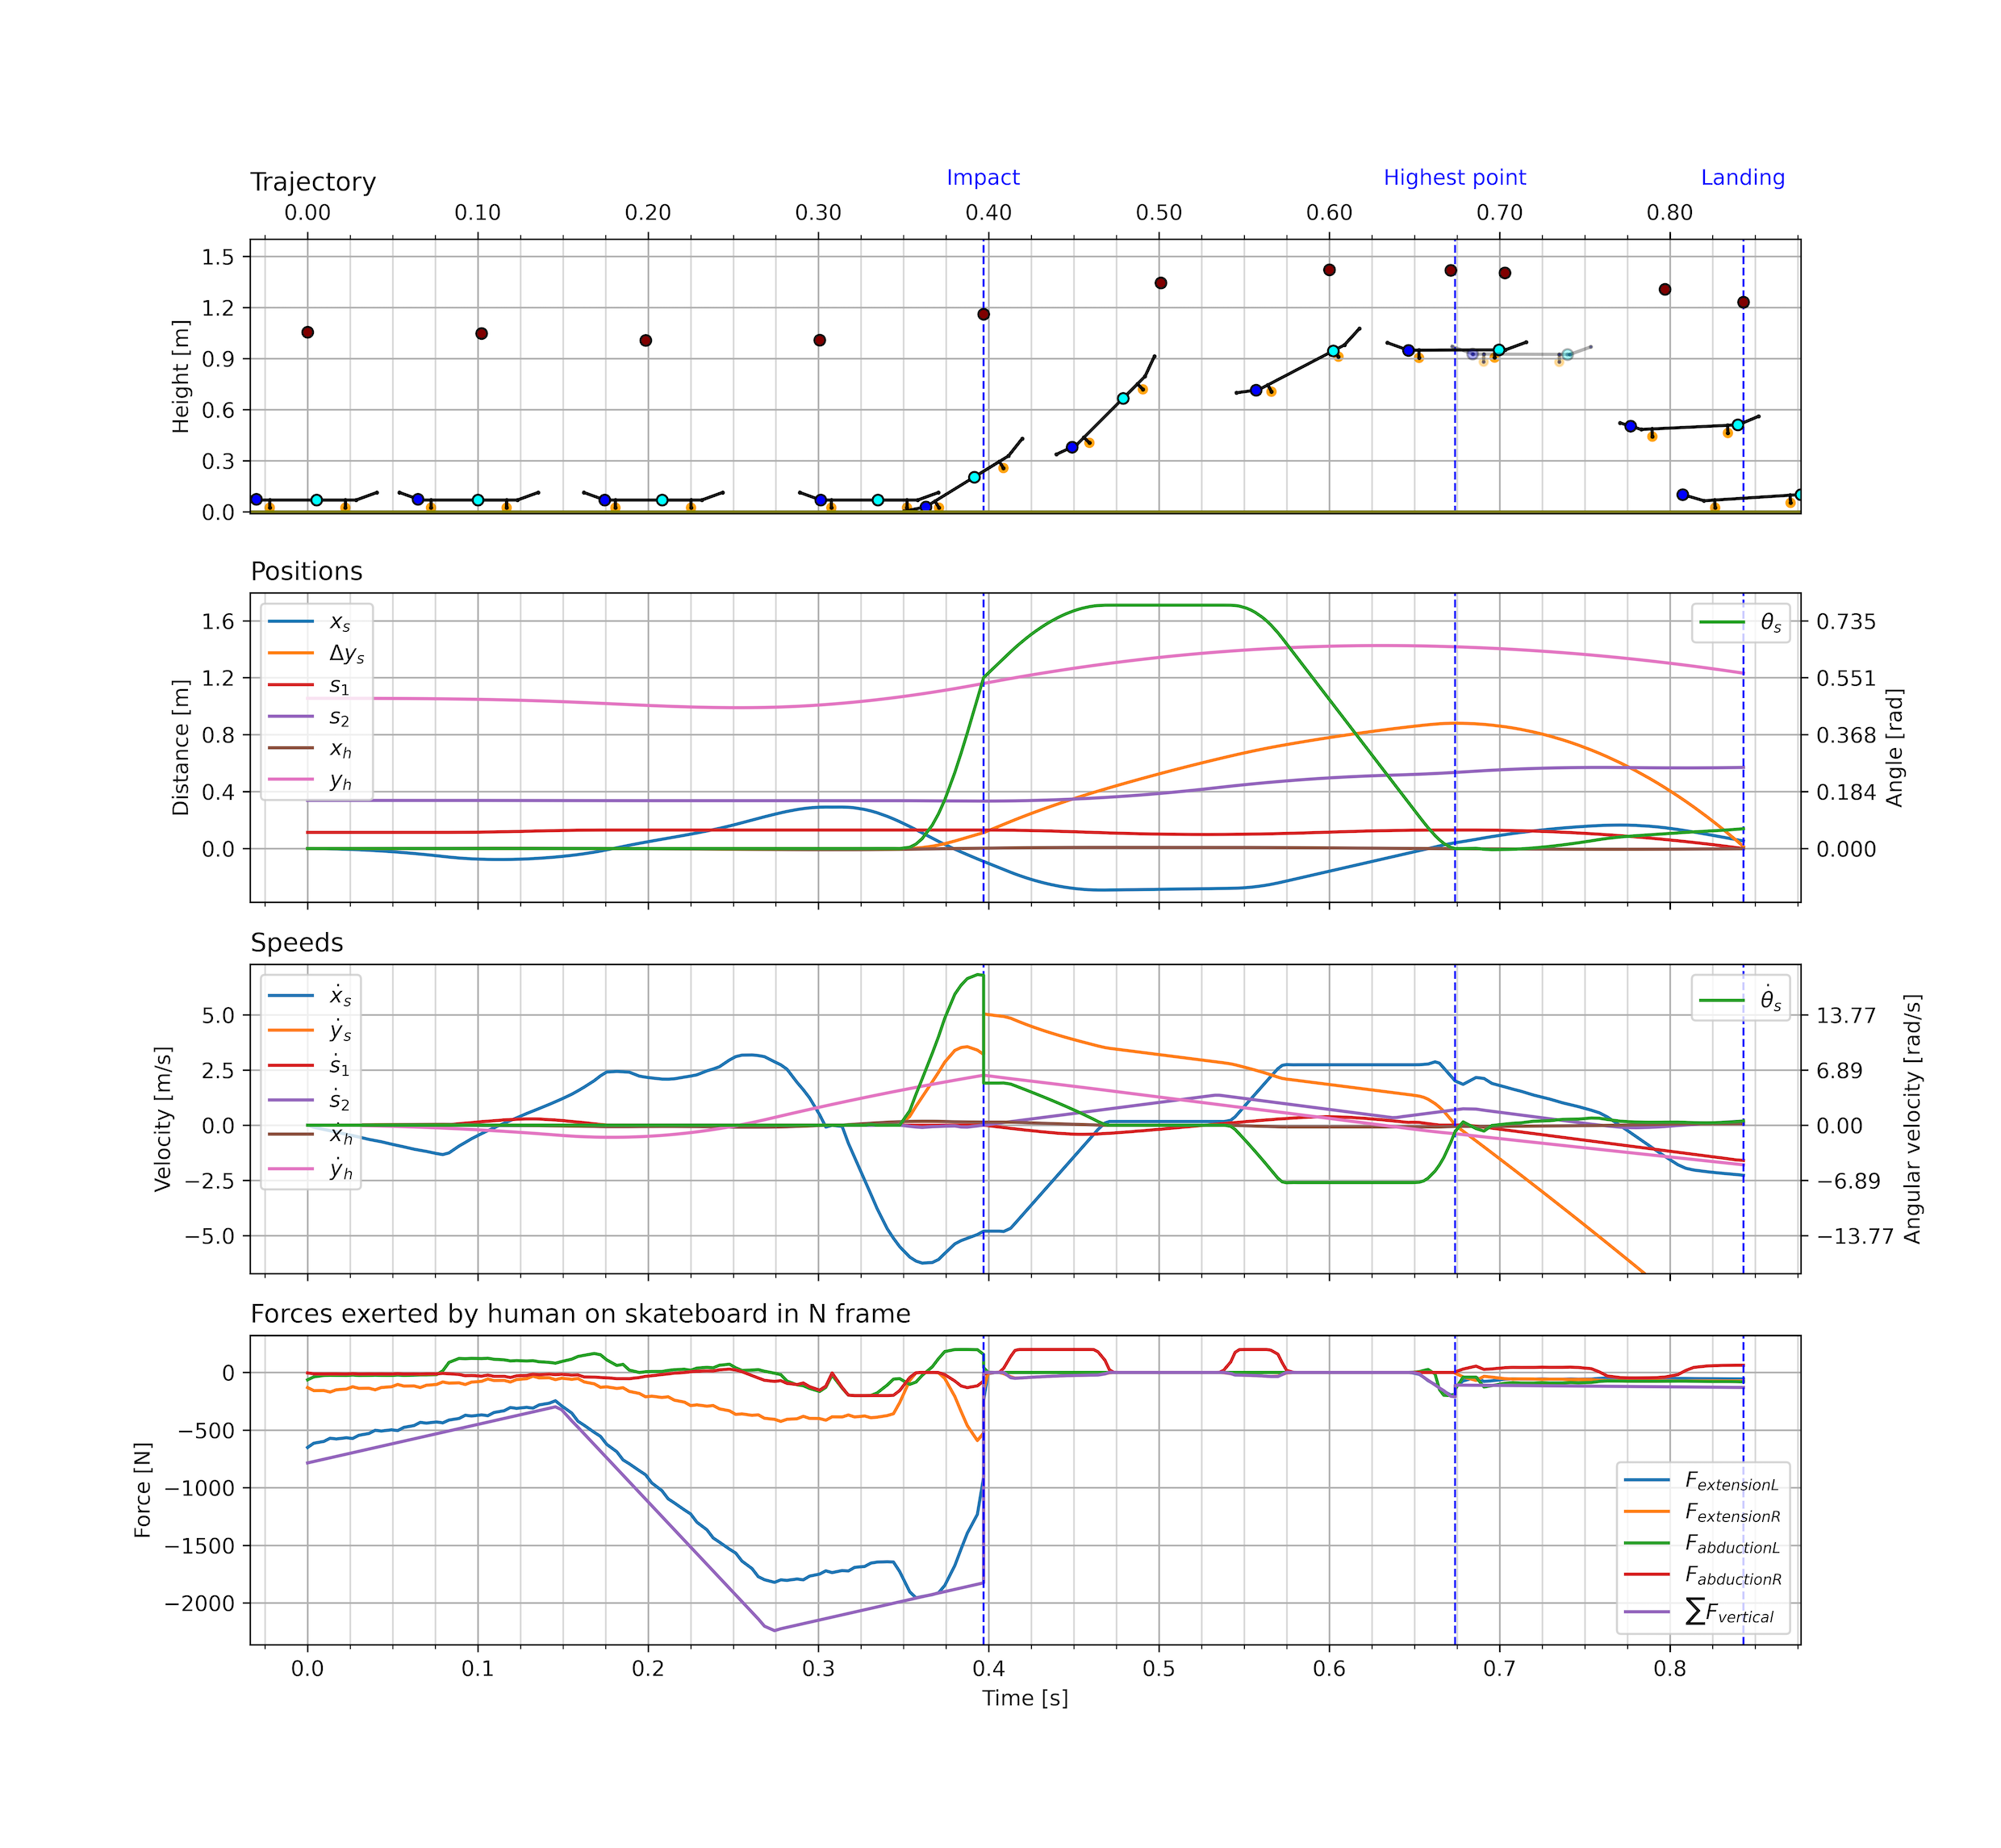
\includegraphics[trim={0cm 0cm 0cm 0cm},clip,width=0.8\textwidth]{figure/Results/data_d_trdpi600.png}}
    \caption{Wheel radius and truck height optimization results}    
\end{figure*}

% \begin{figure*}[b]    
%     \subfloat[Wheel radius]{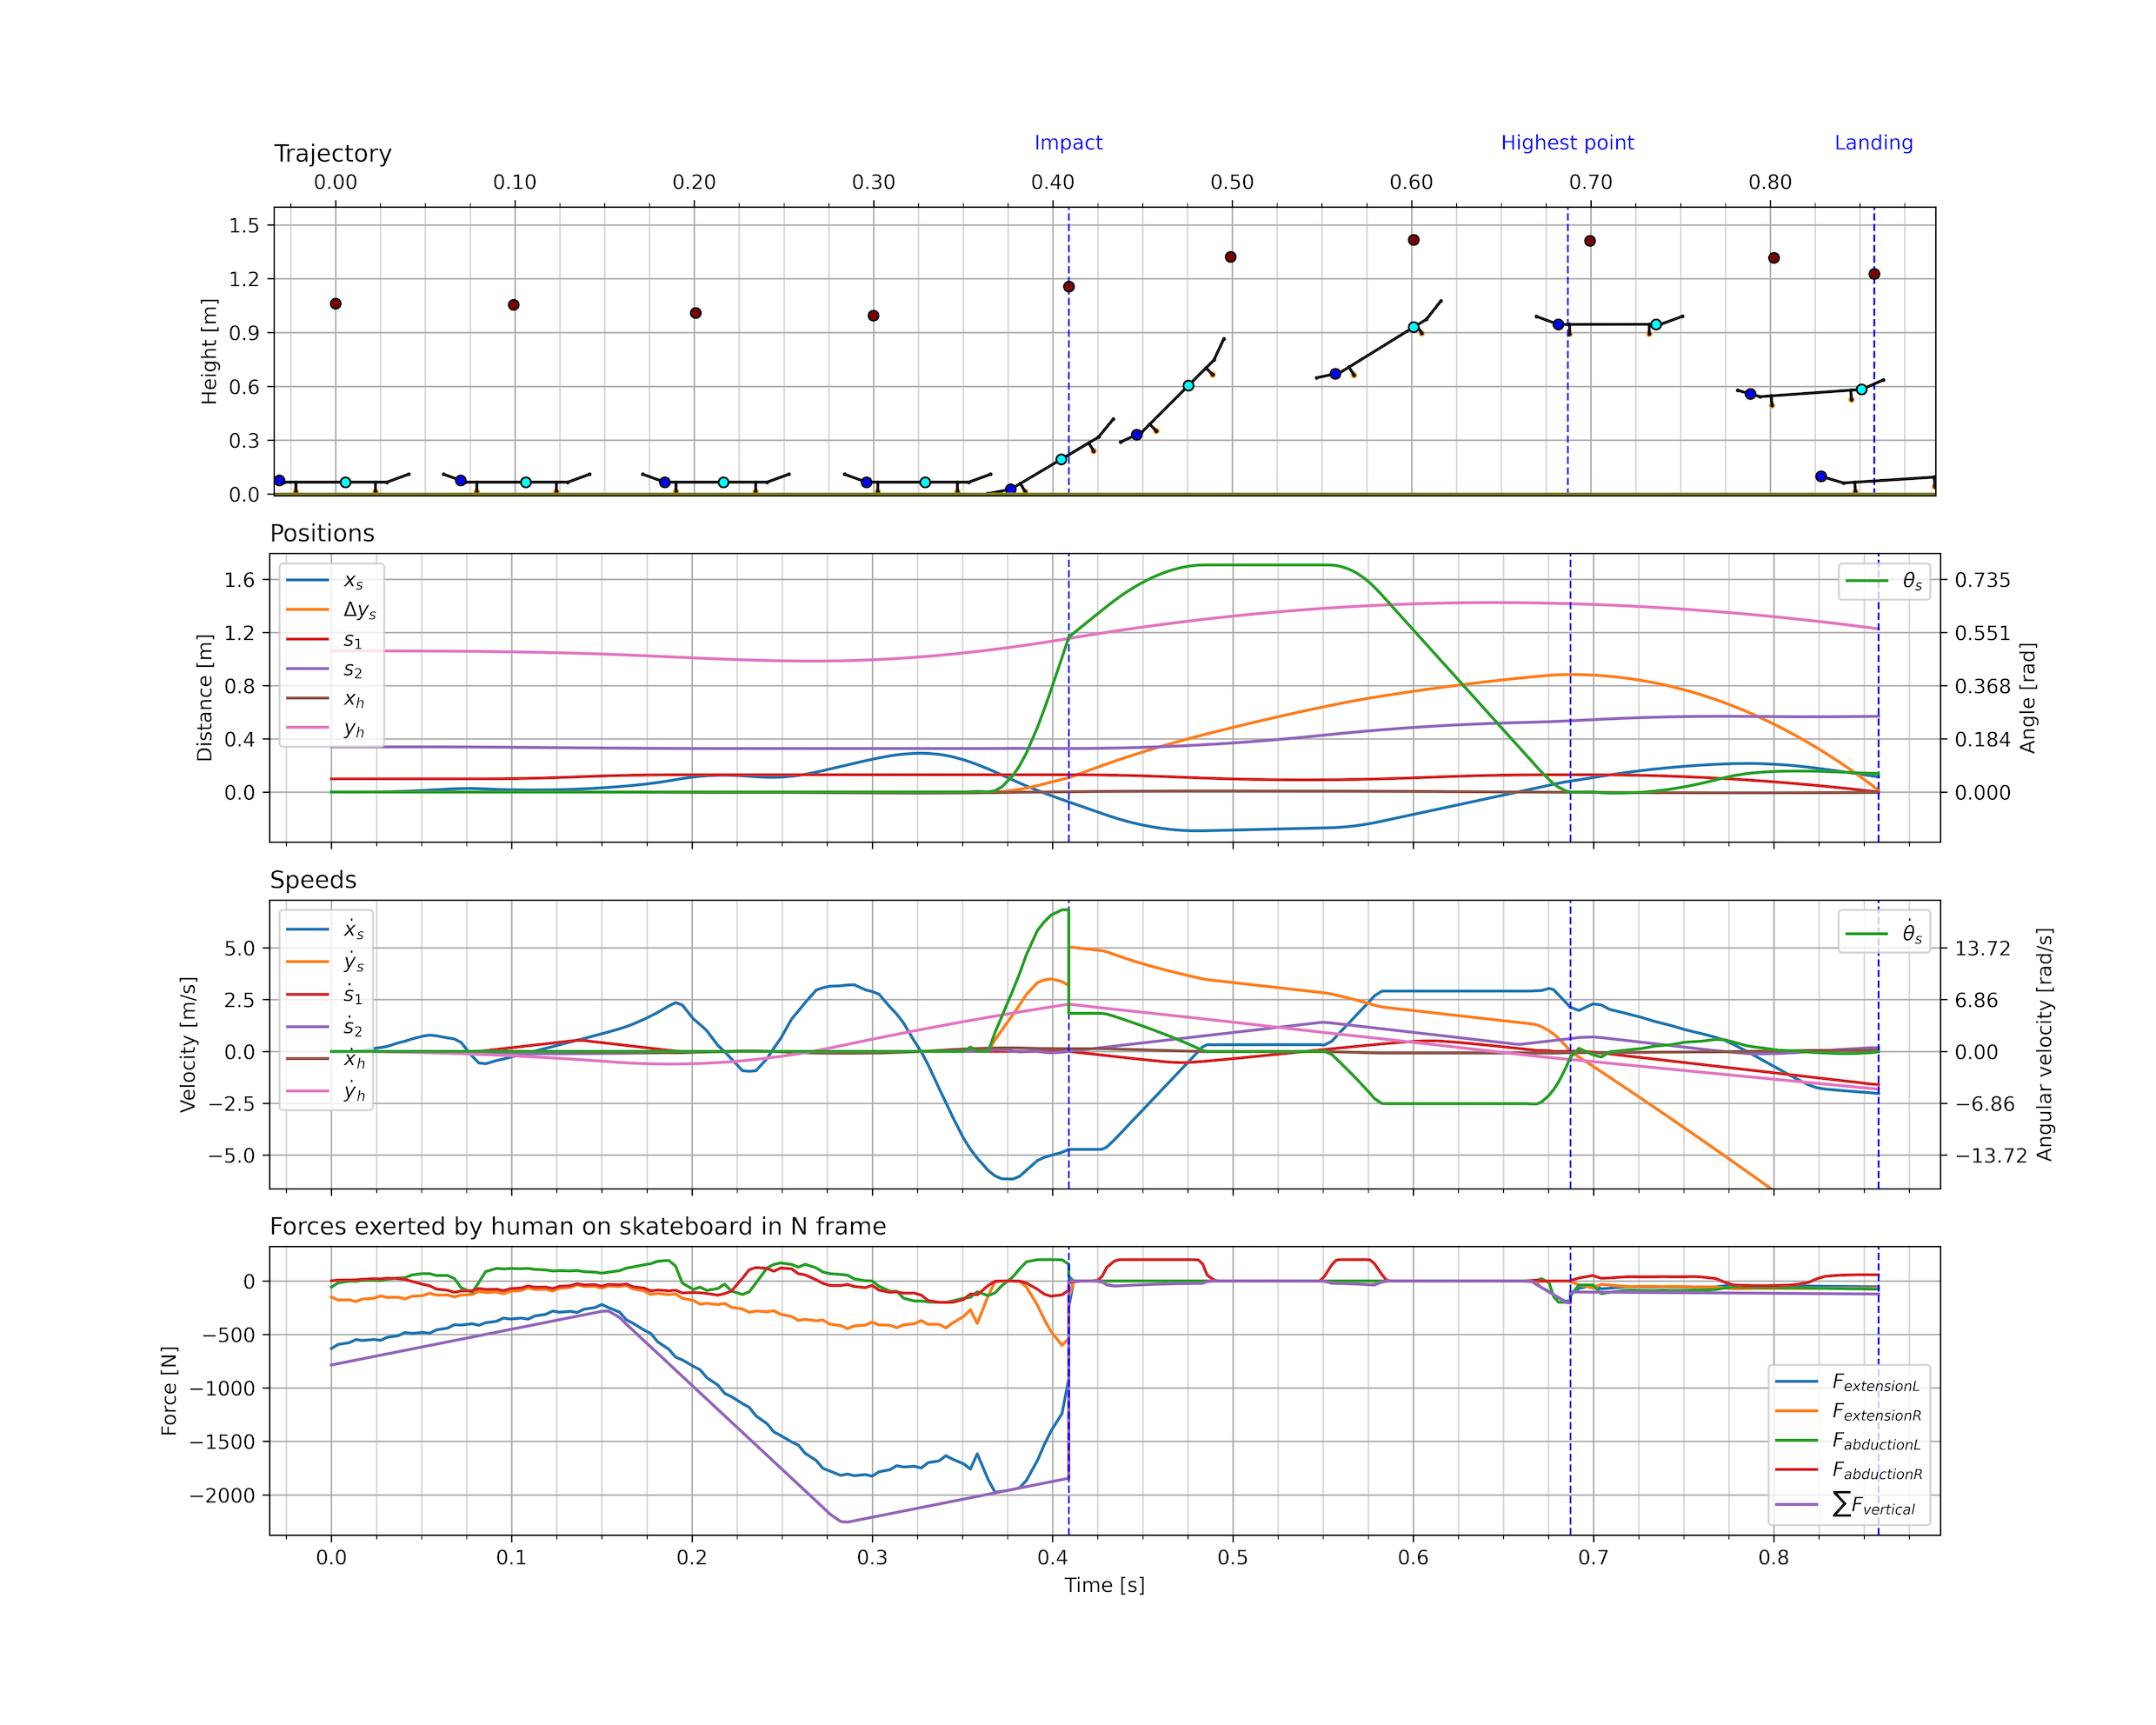
\includegraphics[trim={0cm 0cm 0cm 0cm},clip,width=0.8\textwidth]{figure/Results/data_r_wdpi600.png}}
%     \newline
%     \subfloat[Truck height]{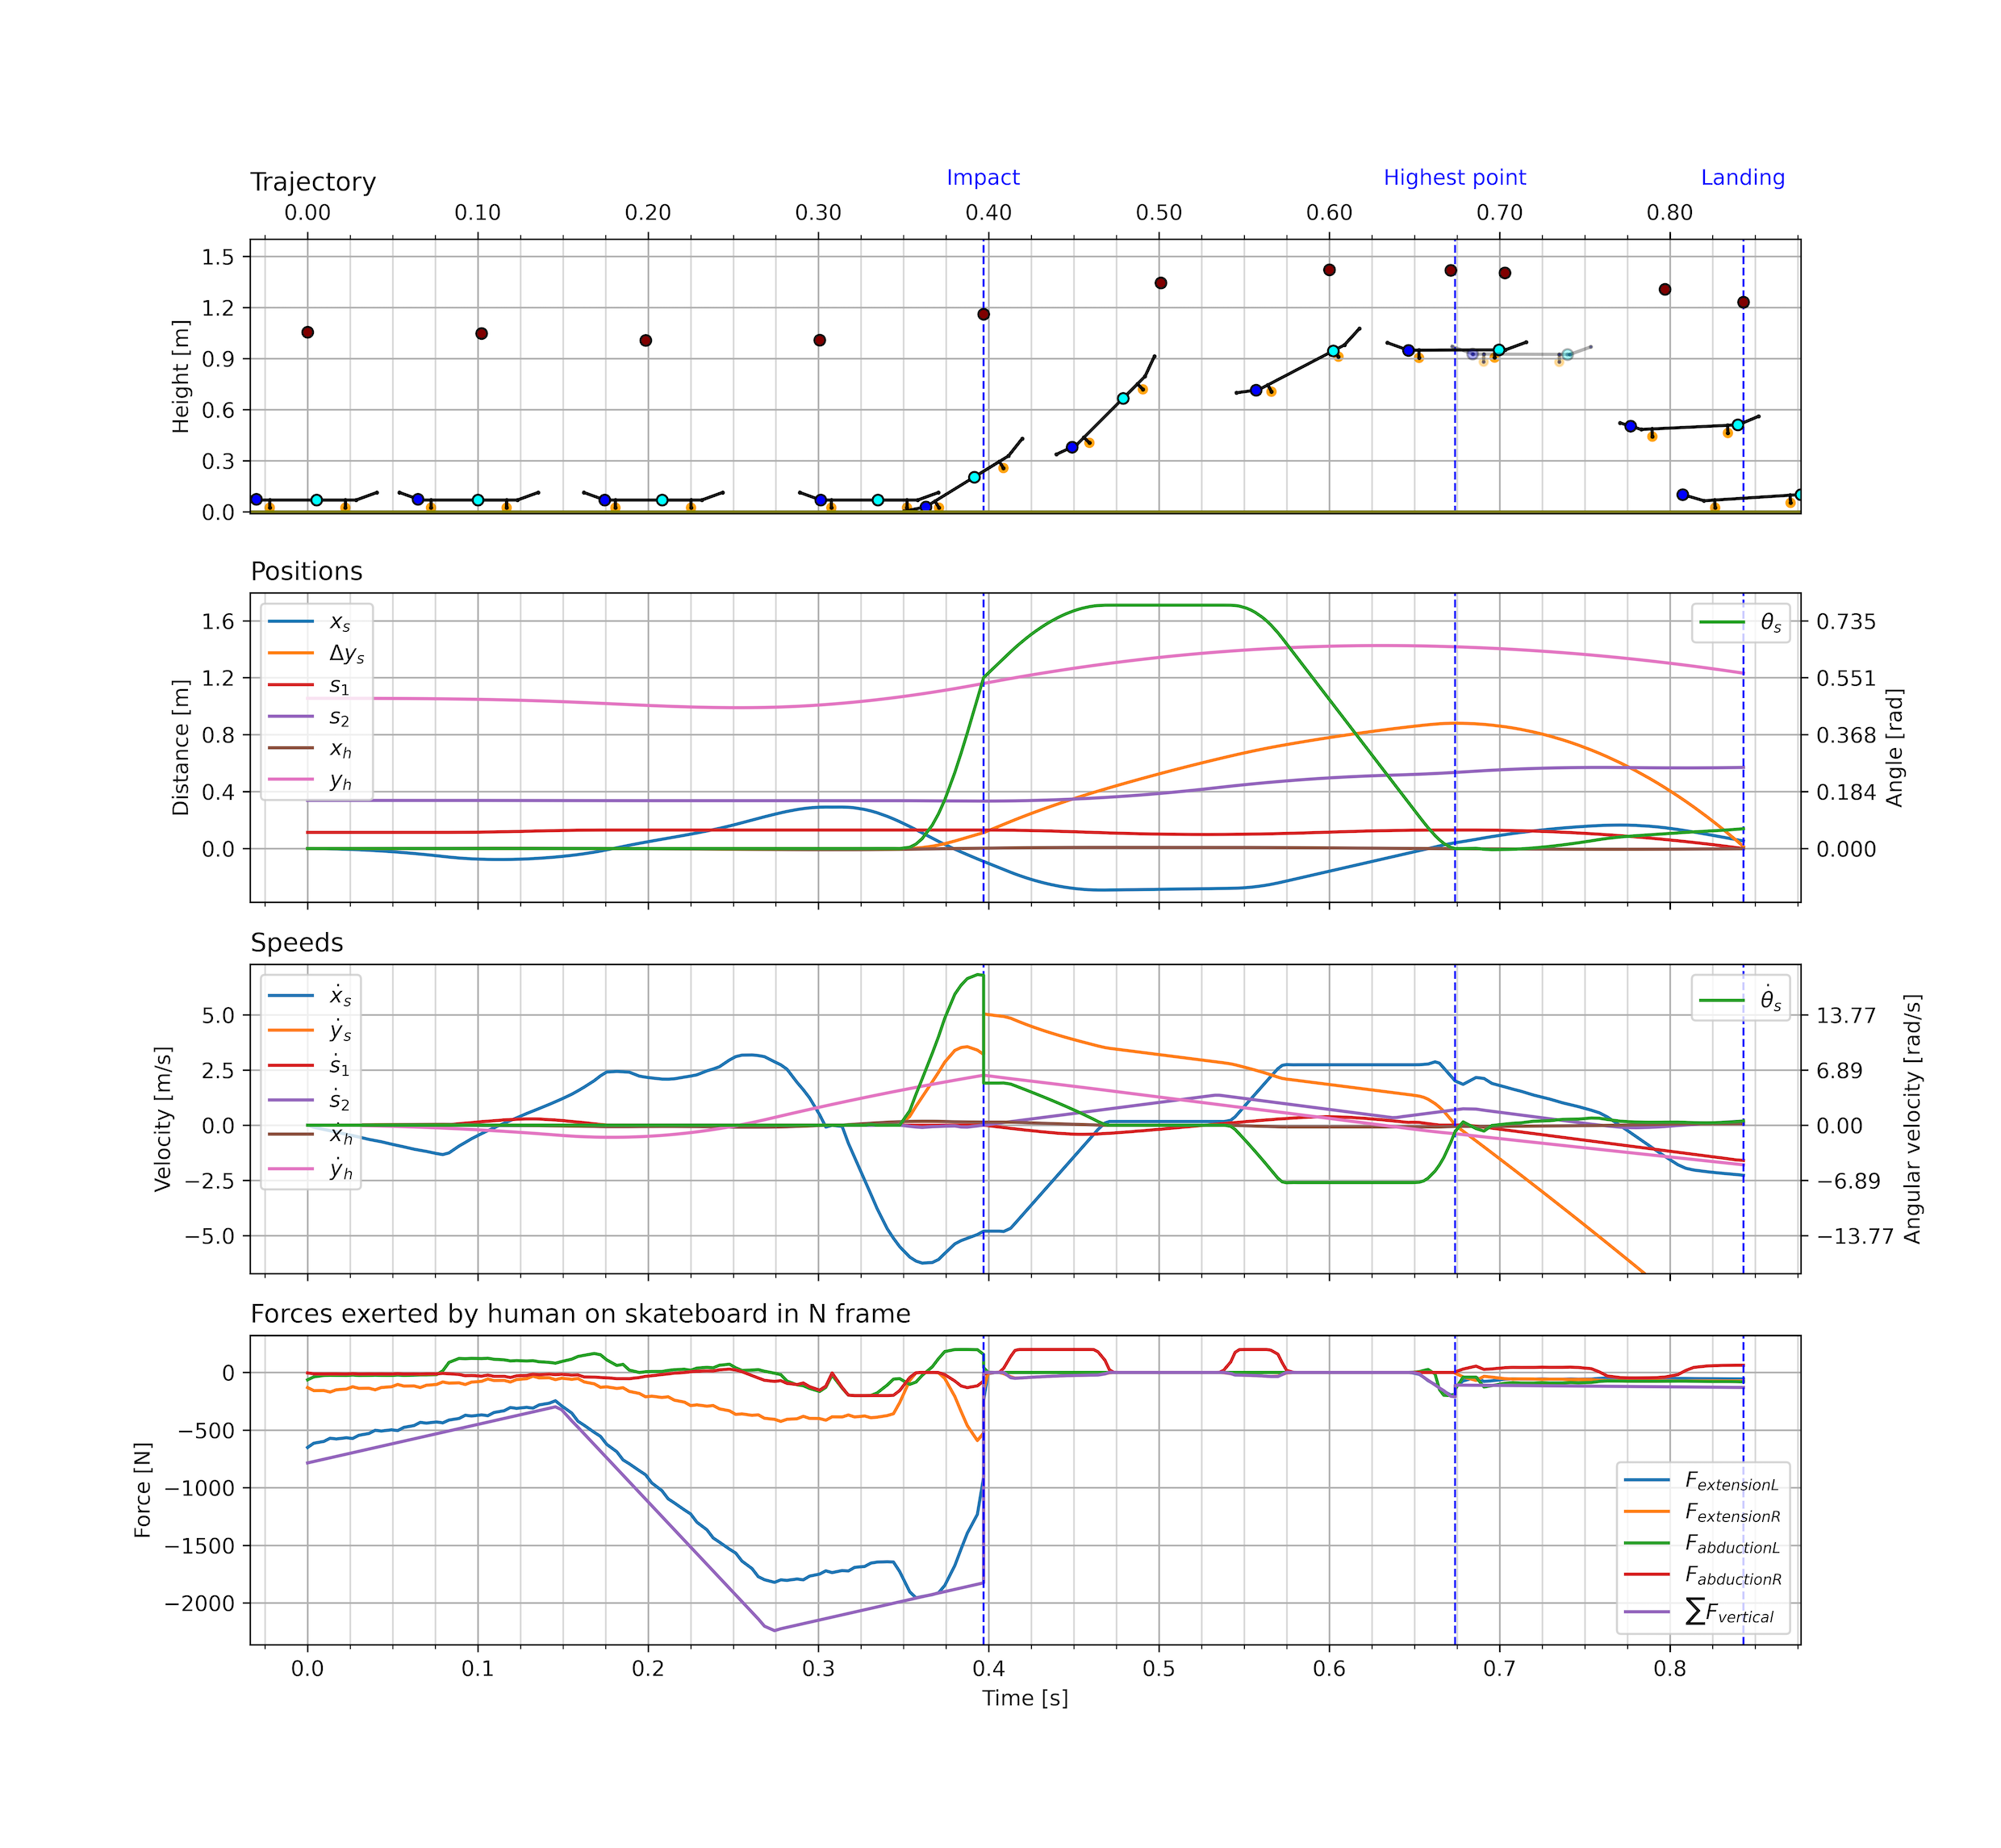
\includegraphics[trim={0cm 0cm 0cm 0cm},clip,width=0.8\textwidth]{figure/Results/data_d_trdpi600.png}}
%     \caption{Single parameter optimization}    
% \end{figure*}

\begin{figure*}[b]    
    \subfloat[Deck length]{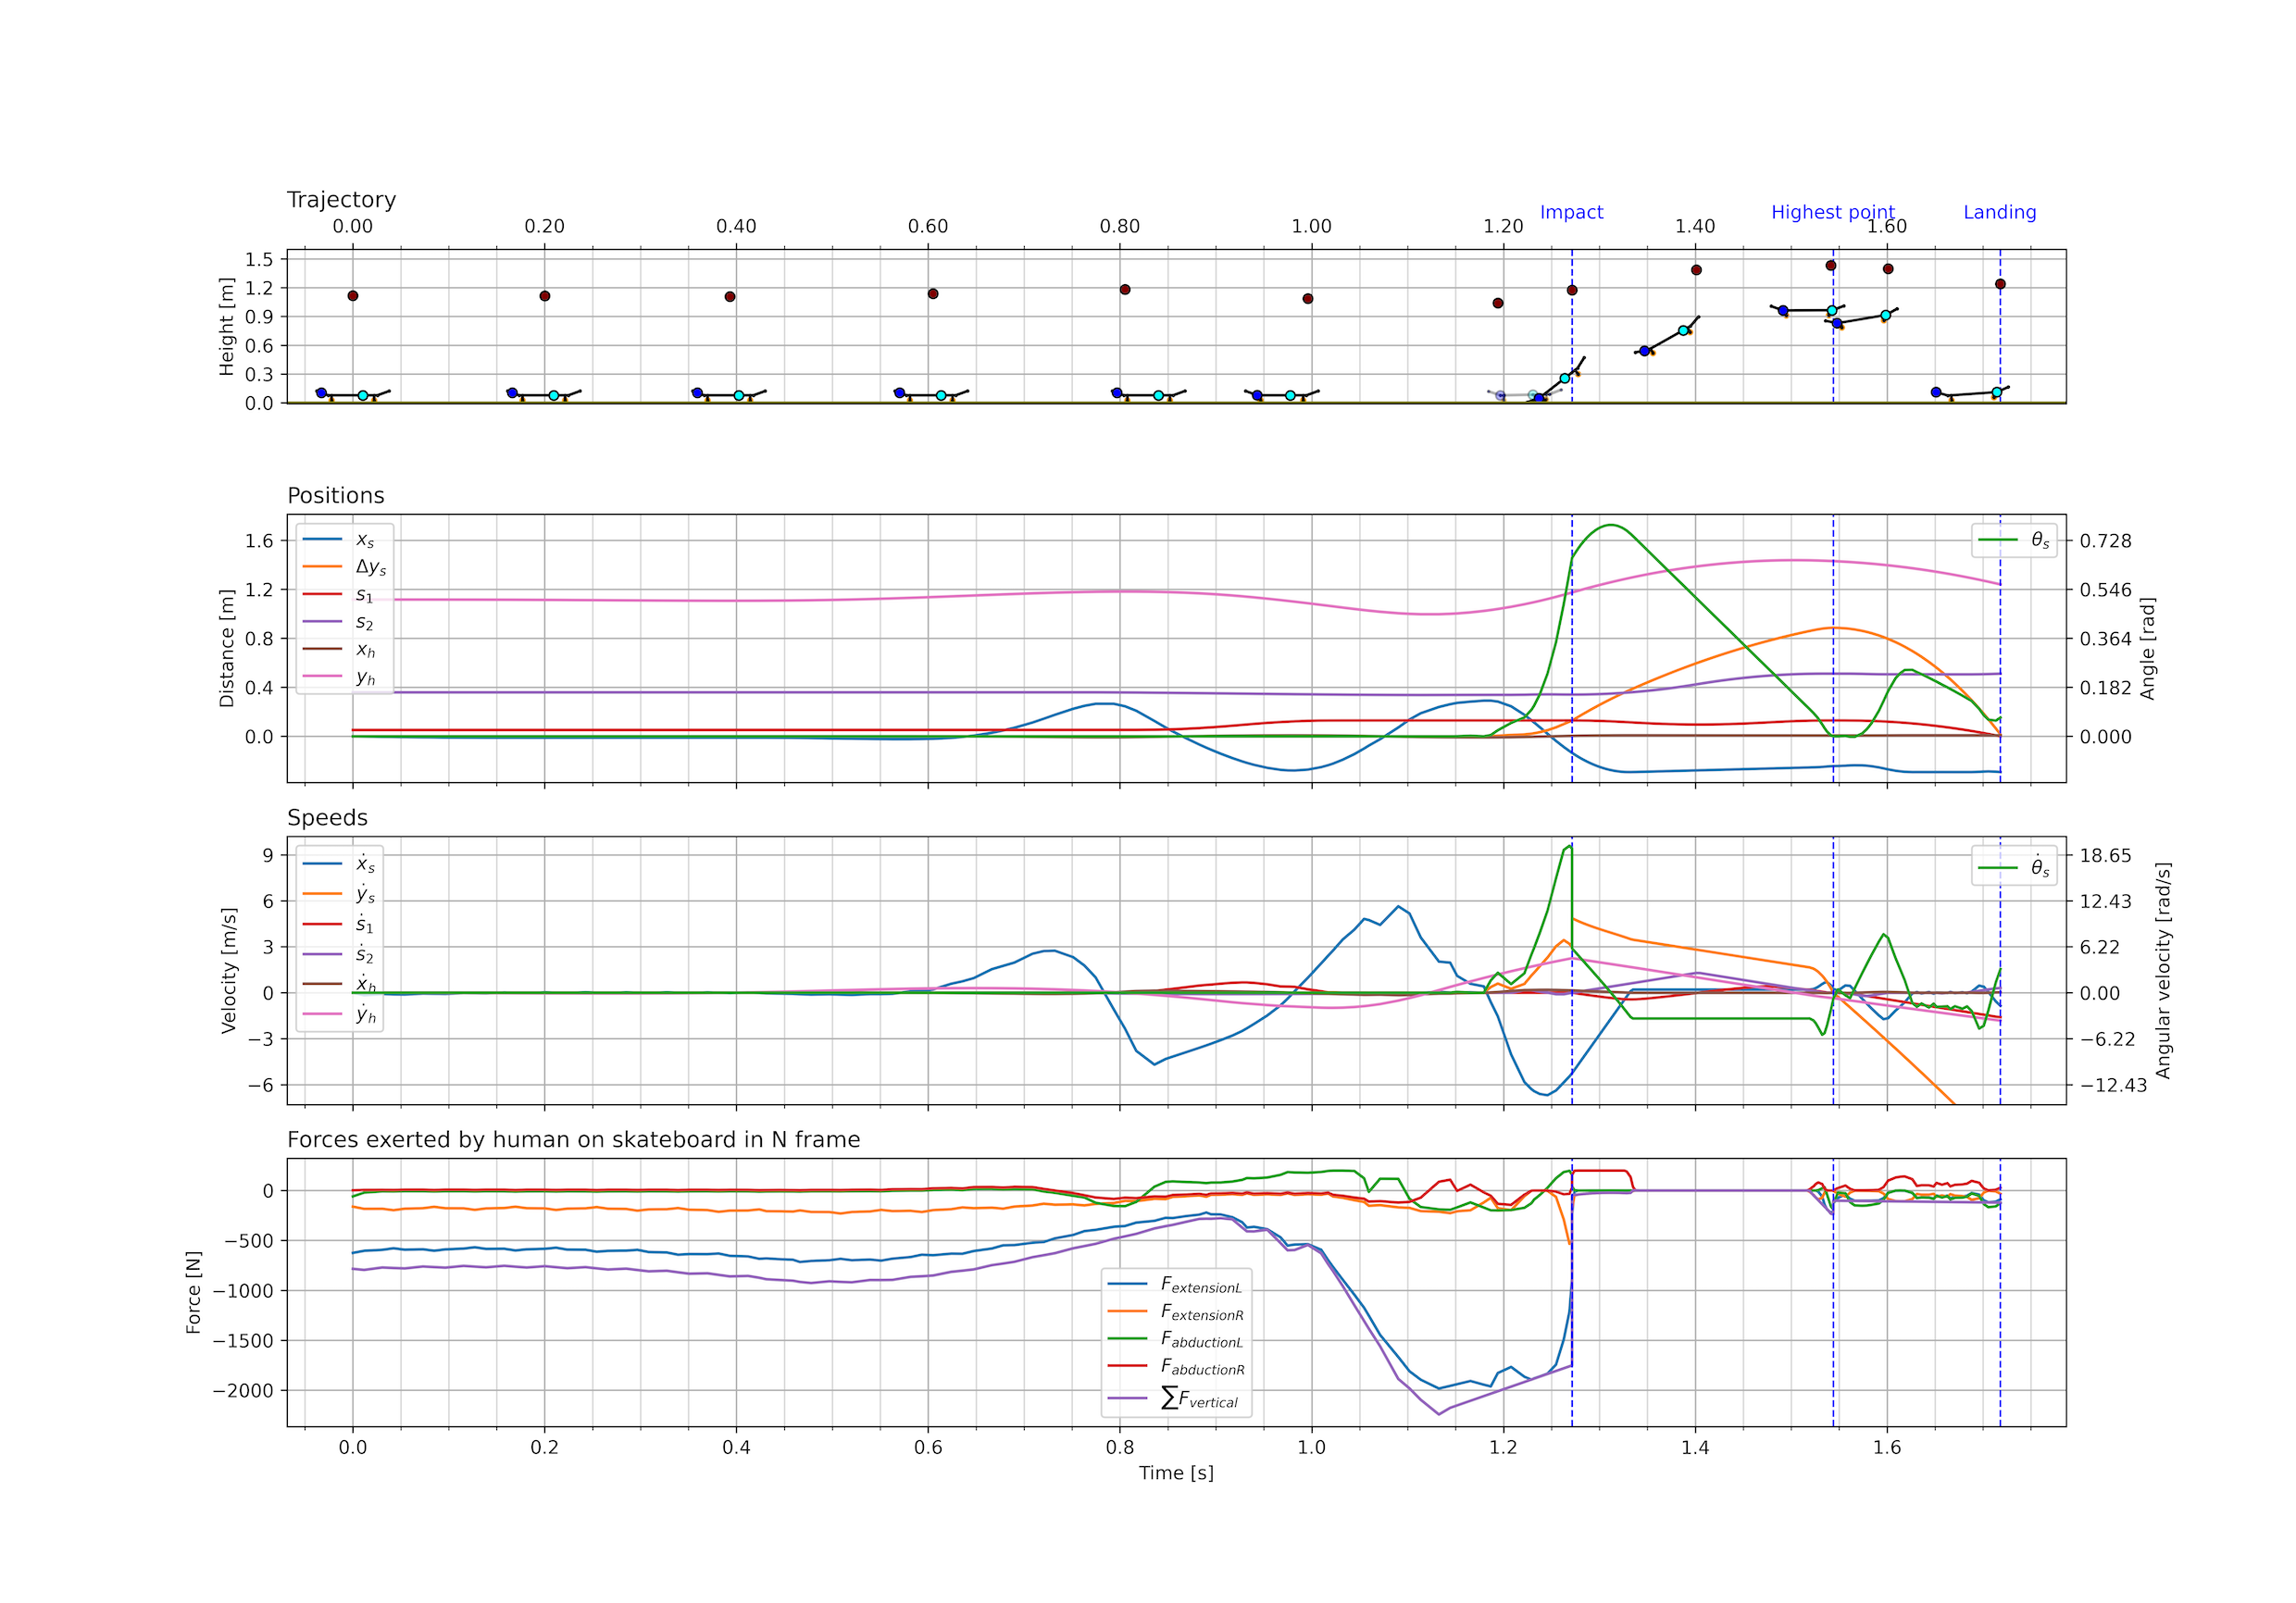
\includegraphics[trim={0cm 0cm 0cm 0cm},clip,width=0.8\textwidth]{figure/Results/data_l_fdpi600.png}}
    \newline
    \subfloat[Tail length]{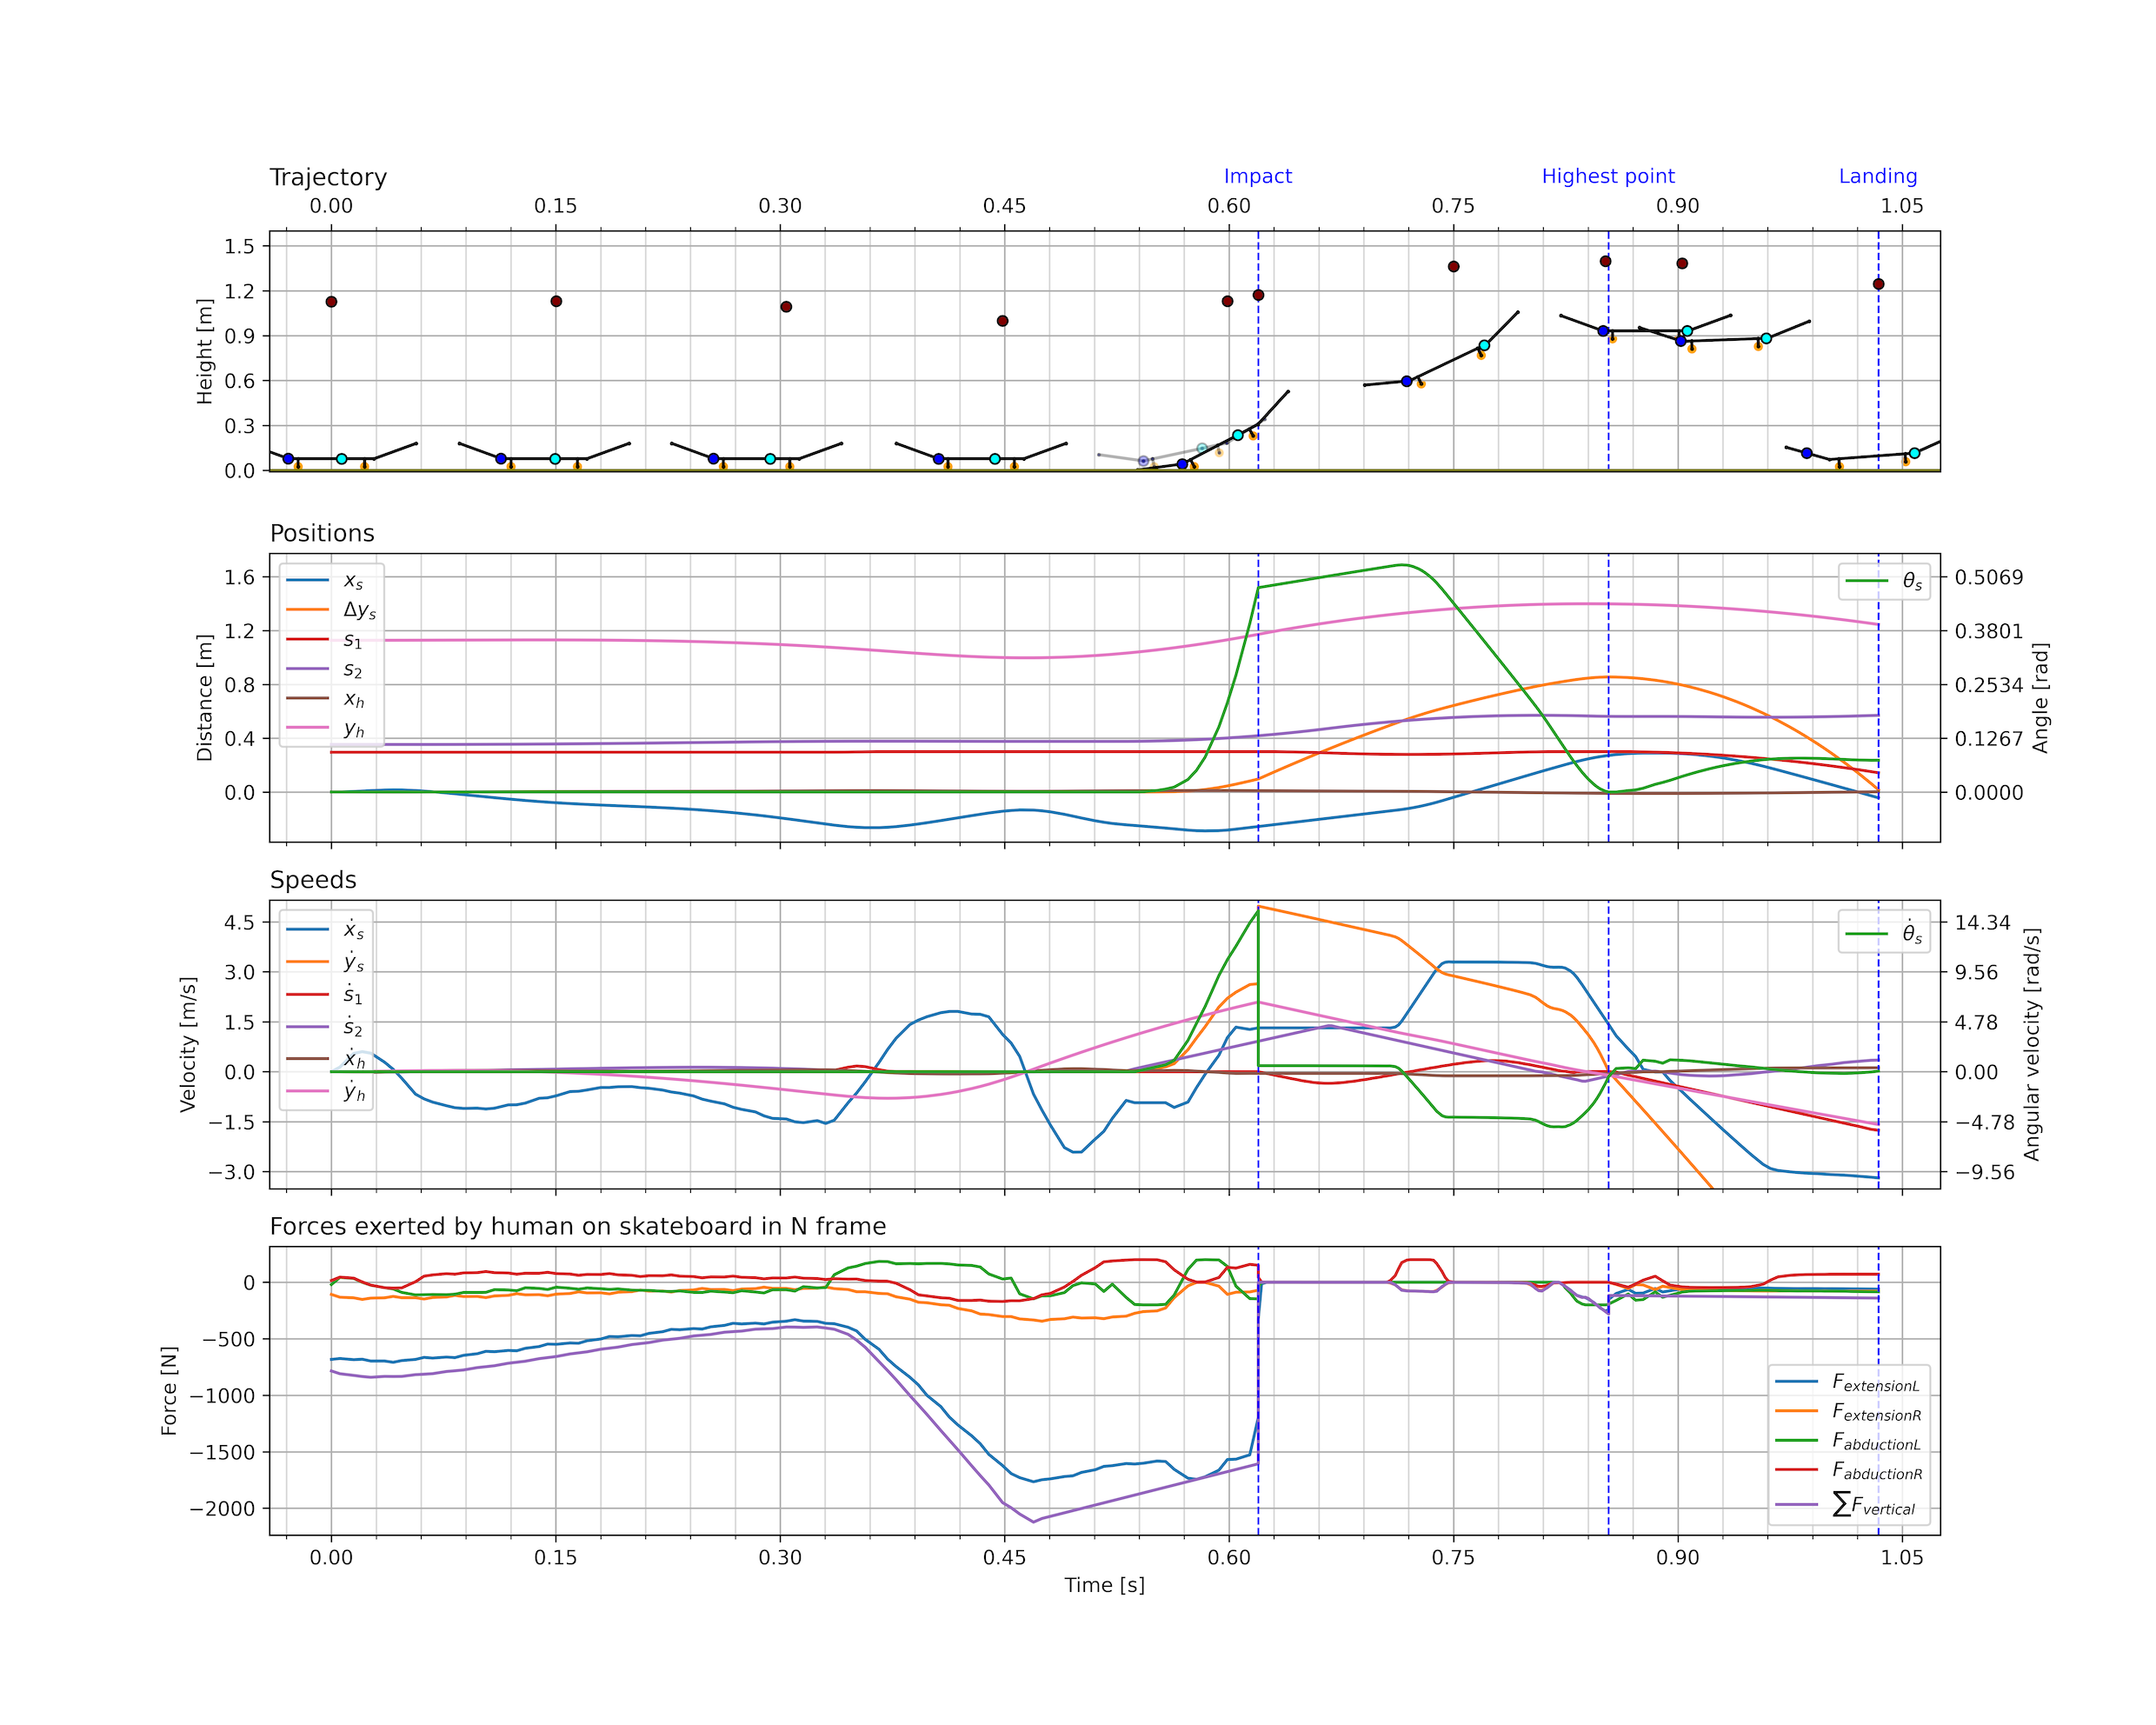
\includegraphics[trim={0cm 0cm 0cm 0cm},clip,width=0.8\textwidth]{figure/Results/data_l_tdpi600.png}}
    \caption{Deck length and tail length optimization results}    
\end{figure*}

\begin{figure*}[b]    
    \subfloat[Tail inclination]{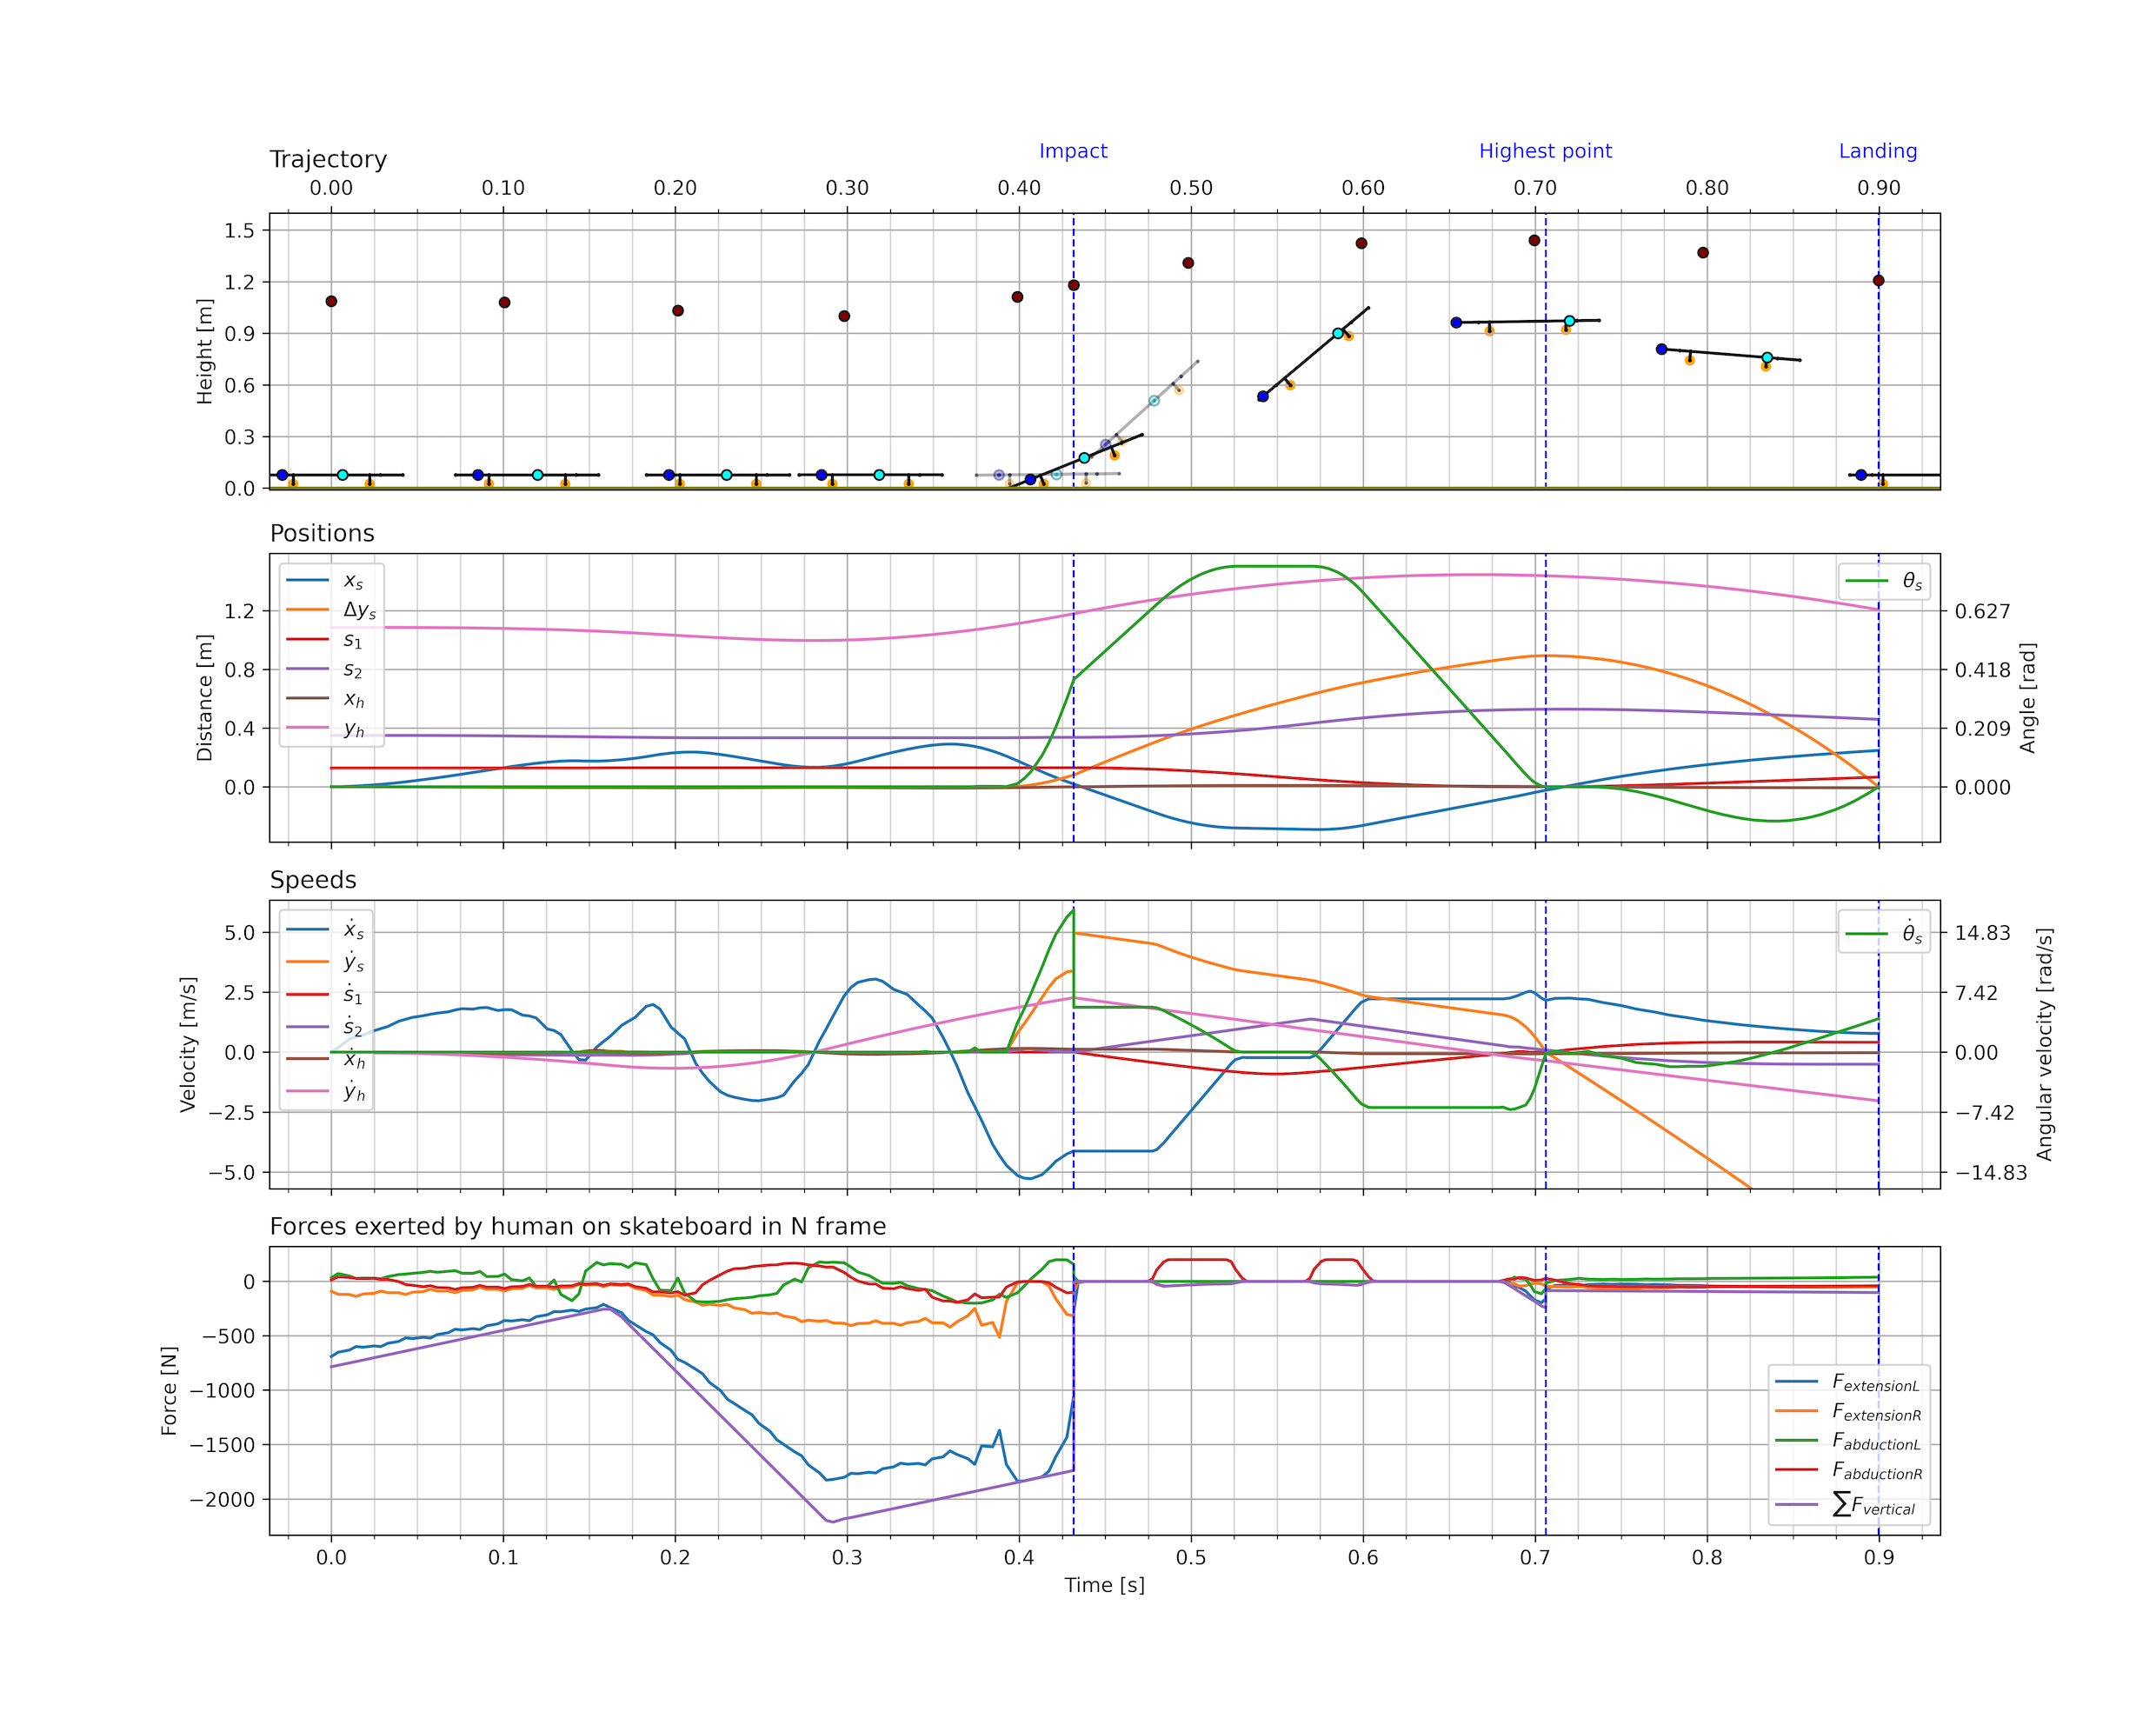
\includegraphics[trim={0cm 0cm 0cm 0cm},clip,width=0.8\textwidth]{figure/Results/data_phidpi600.png}}
    \newline
    \subfloat[All parameters]{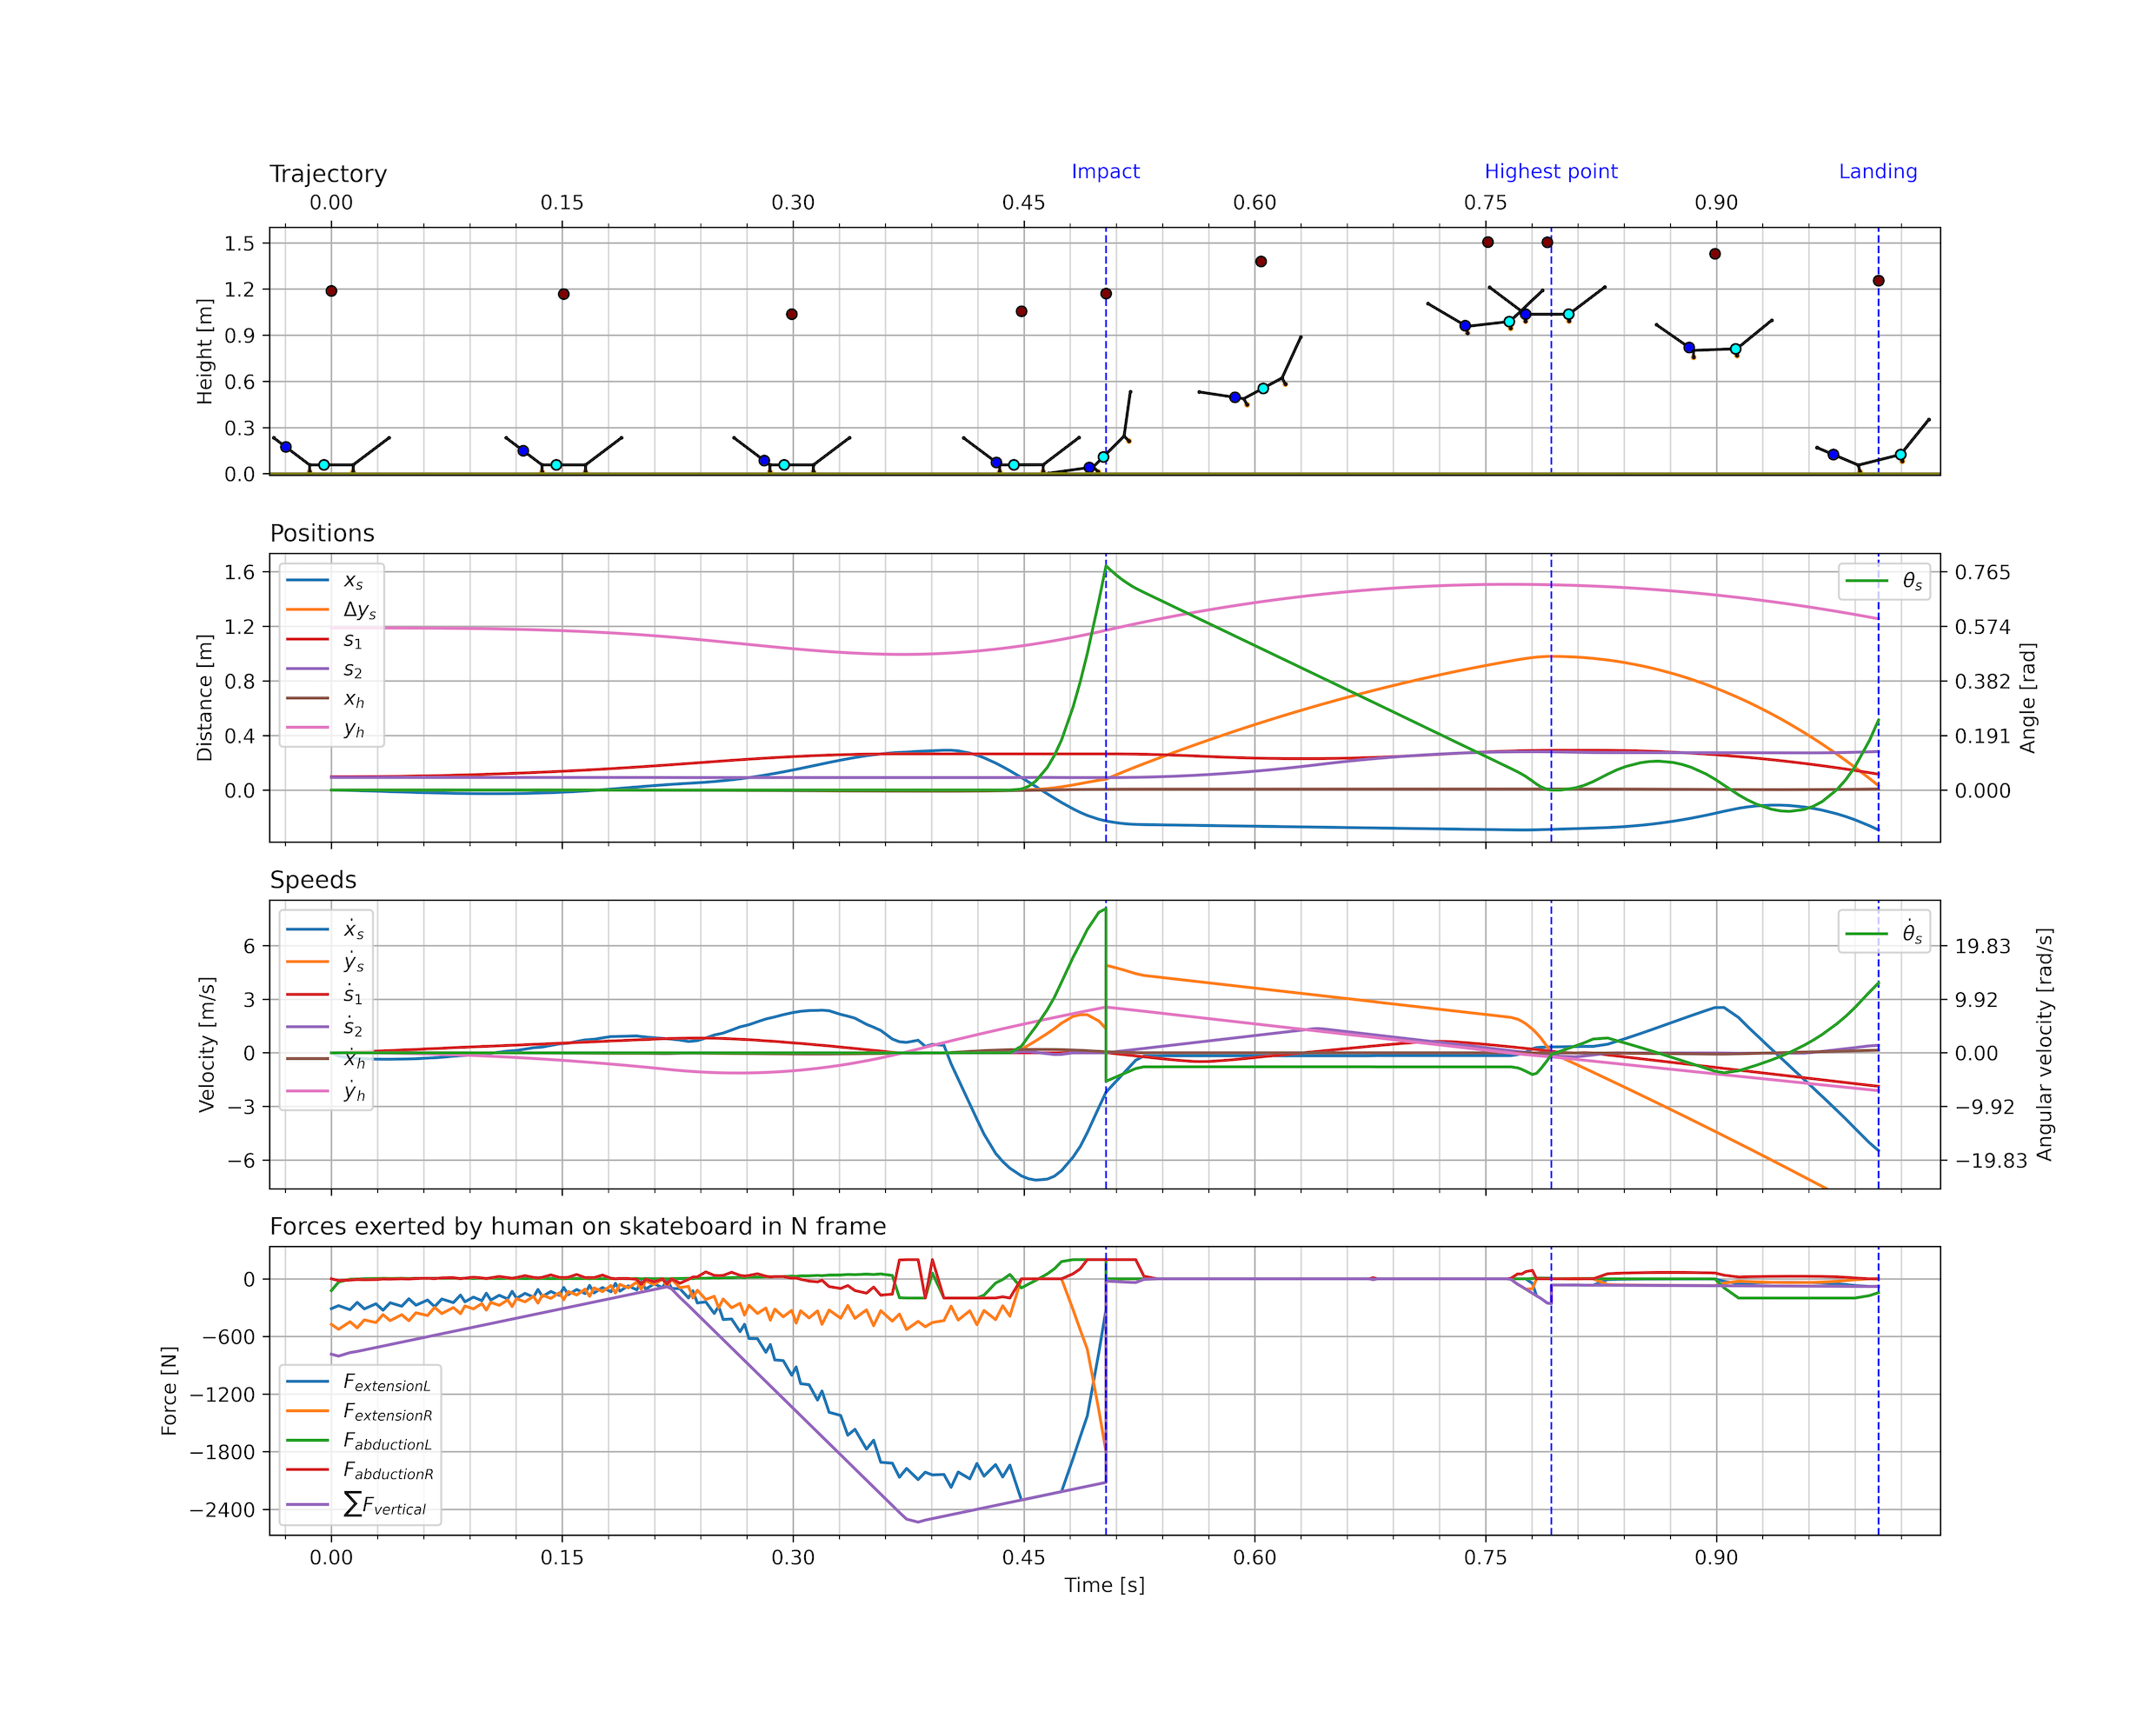
\includegraphics[trim={0cm 0cm 0cm 0cm},clip,width=0.8\textwidth]{figure/Results/data_alldpi600.png}}
    \caption{Tail inclination and all parameters optimization results}    
\end{figure*}


%Appendix will include inertia experiments and friction experiments

%% SHOW THAT NOSE ISN'T USED WHEN THE POSSIBILITY IS THERE

%% SHOW HOW VELOCITIES AFTER IMPACT ARE CALCULATED

%% SHOW 3 Friciton models
% During impact, friction can be present when there is a tangential velocity state relative to the impact surface. Poissons method and Newtons method have been shown unaccurate for such events and it is advised to use Stronge's method. This has been shown numerically in Stronge's comment on collision with friction\cite{stronge_comment_2010}. When the tail of the skateboard hits the ground, usually there is a tangential velocity state at the location of impact. This means that in real life a frictional impact occurs. Another implementation of the Poisson method during a frictional impact is solved with a set of constraints in the optimization\cite{patel_contact-implicit_2019}. The theory is that you create a variable $\phi(q_i)$, that represents the distance from the contact surface dependant on the generalized coordinates which should always be greater than 0. Furthermore there are three forces that should obey the friction cone presented in 

\end{document}
